\documentclass[a4paper,10pt]{article}
\usepackage{graphicx}
\usepackage{float}
\usepackage{booktabs}
\usepackage{amsmath}
\usepackage{amssymb}
\usepackage{amsthm}
\usepackage{physics}
\usepackage{geometry}
\usepackage{latexsym}
\renewcommand{\figurename}{Figura}
\newcommand*{\unit}[1]{\ensuremath{\mathrm{\,#1}}}
\geometry{a4paper,tmargin=4cm,bmargin=3.5cm, lmargin=3cm,rmargin=3cm}

\title{High-Purity germanium detectors}
\author{Gianluca Cavallaro \\ Marco Gobbo}
\date{20 Aprile 2020}
\begin{document}
\maketitle

%%% INTRODUZIONE E PRESUPPOSTO TEORICO %%%

\section{Introduzione}
La seguente esperienza ha come scopo quello di studiare la caratterizzazione di due diversi rivelatori al germanio. Per avere un quadro pi\`u completo, illustriamo brevemente le caratteristiche di questi tipi di rivelatori. Si tratta di una classe di rivelatori a semiconduttore, il germanio in questo caso, che sfrutta la tecnologia della giunzione P-N. La giunzione P-N \`e costituita da due zone: una con un eccesso di lacune ed una con un eccesso di elettroni. Lacune ed elettroni vengono ottenuti mediante diverse tecniche di drogaggio del materiale utilizzato. La zona chiave della giunzione P-N \`e quella di confine tra le due zone: i portatori di carica possono diffondere nella zona adiacente, attraverso una corrente di diffusione, creando, in ultima istanza, una differenza di potenziale che genera un campo elettrico, il quale a sua volta genera una corrente di trascinamento che si oppone a quella di diffusione. Le caratteristiche delle due zone e dei portatori di carica dipendono dalle caratteristiche costitutive della giunzione. La giunzione pu\`o poi essere sottoposta a polarizzazione diretta o inversa: nel nostro caso siamo interessati a polarizzare inversamente la giunzione, cos\`i che nel nostro rivelatore non ci sia nessuna corrente sovrapposta a quella di raccolta delle cariche. Il rivelatore va poi tenuto in un dewar che lo mantiene ad una temperatura di 77K, attraverso un bagno di azoto liquido. Questo perch\'e nei semiconduttori la banda di valenza e di conduzione sono separate da un gap in energia: nel germanio il gap \`e talmente basso (0.67 eV) che mantenendo il rivelatore a temperatura ambiente l'agitazione termica sarebbe sufficiente a superarlo, ostacolando le nostre misure.
\section{Parte 1}

%%% STRUMENTAZIONE PRIMA PARTE %%%

\subsection{Strumentazione}
\begin{itemize}
\item Crate NIM per alimentazione di elettronica standard
\item Rivelatore coassiale HPGe (Ortec Coaxial HPGe Detector GEM20P)
\item Generatore HV Label Model 8124 per tensione di polarizzazione
\item Amplificatore CAEN Model N968
\item ADC/MCA CAEN Model N957
\item Sorgenti di calibrazione: 22Na, 60Co, 228Th
\end{itemize}

%%% SCELTA DEI MIGLIORI VALORI DI TENSIONE E SHAPING TIME %%%

\subsection{Scelta delle condizione ottimali di lavoro}
Il segnale \`e acquisito mediante una catena di lettura classica. In questo caso abbiamo un dispositivo che integra detector e pre-amplificatore, uno che integra amplificatore e shaper e un ADC/MCA a parte. L'obiettivo di questa prima parte \`e quello di individuare le condizioni ottimali per tensione di polarizzazione e shaping time per proseguire nell'esperienza. Individuare le condizioni di lavoro ottimali significa individuare quelle che minimizzano la risoluzione. Abbiamo a nostra disposizione degli spettri di una sorgente di 22Na, raccolti in corrispondenza di diversi valori di polarizzazione, da 2000V a 5000V, e di shaping time, rispettivamente 0.5, 1, 2, 3, 6, e 10 $\mu$s. Di seguito sono riportati un esempio di High Voltage e Shaping Time (i restati sono in Appendice).

\begin{figure}[!h]
    \centering
    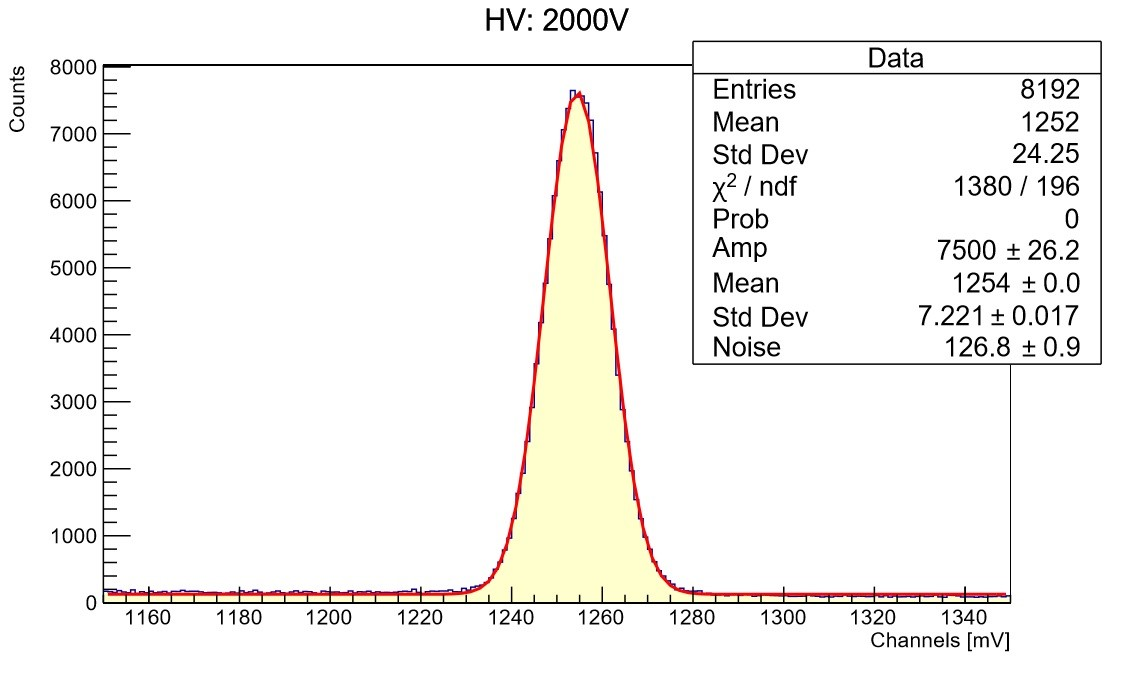
\includegraphics[scale=0.6]{grafici/hv}
    \caption{Tensione di polarizzazione 2000V}
\end{figure}

\begin{figure}[!h]
    \centering
    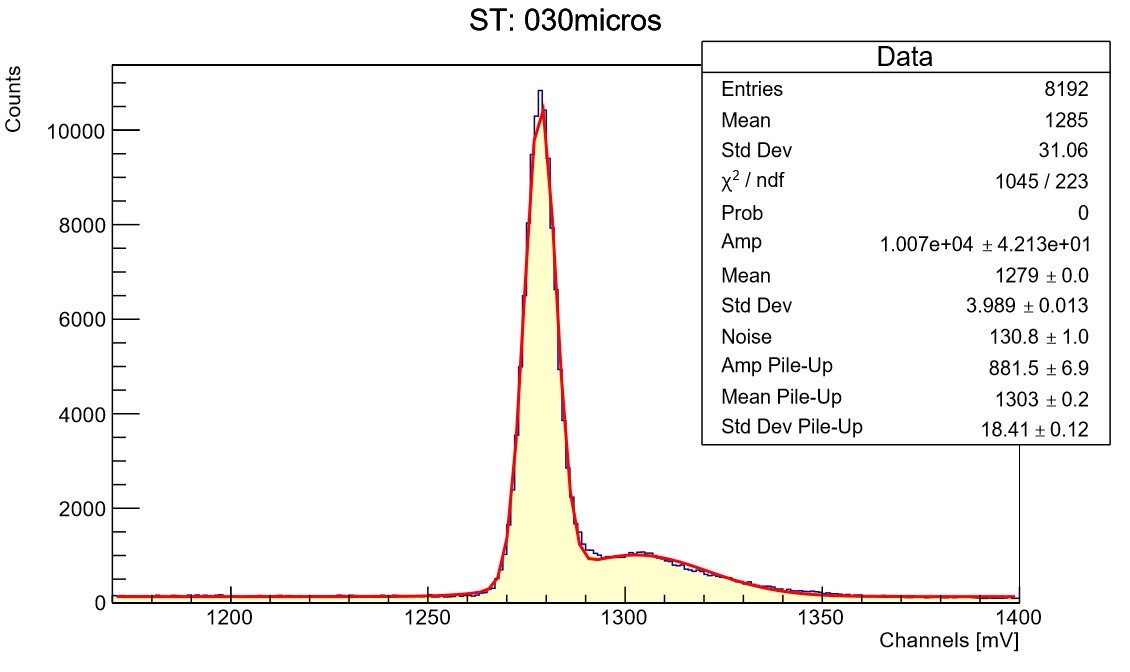
\includegraphics[scale=0.6]{grafici/st}
    \caption{Shaping time 30 $\mu$s}
\end{figure}

\noindent Per i grafici relativi alla tensione di polarizzazione \`e stato necessario effettuare uno "zoom" nella regione dove si registra il picco. In questa zona, il picco \`e stato estrapolato attraverso una funzione gaussiana sommata ad un polinomio di grado 0, che tiene conto del fondo. Nei grafici relativi allo shaping time il procedimento \`e stato analogo, ma nell'interpolare la funzione \`e stato necessario considerare, oltre al polinomio di grado 0 che continua a considerare il fondo, due gaussiane, con la seconda che ci ha permesso di considerare nel fit il contributo dovuto al pile-up, fenomeno per il quale il rivelatore non \`e "pronto" a ricevere due misure successive, e va quindi a sommare un evento sulla coda di quello precedente, andando in alcuni casi a deformare il picco in questione. Possiamo osservare dunque che le assunzioni sugli andamenti delle distribuzionei sono quasi corrette dal momento che i valori di $\chi^2$-ridotto non sono eccessivamente alti. Attraverso questo processo siamo arrivati ad avere a disposizione 16 valori per la tensione di polarizzazione e 6 per lo shaping time. Per entrambe le raccolte dati, andiamo a costruire il grafico della risoluzione in funzione della tensione di polarizzazione e dello shaping time, rispettivamente. La risoluzione \`e stata calcolata con la seguente relazione: 

\begin{equation}
	R=\frac{\textrm{FWHM}}{\textrm{Channel}}
\end{equation}

\begin{figure}[!ht]
    \centering
    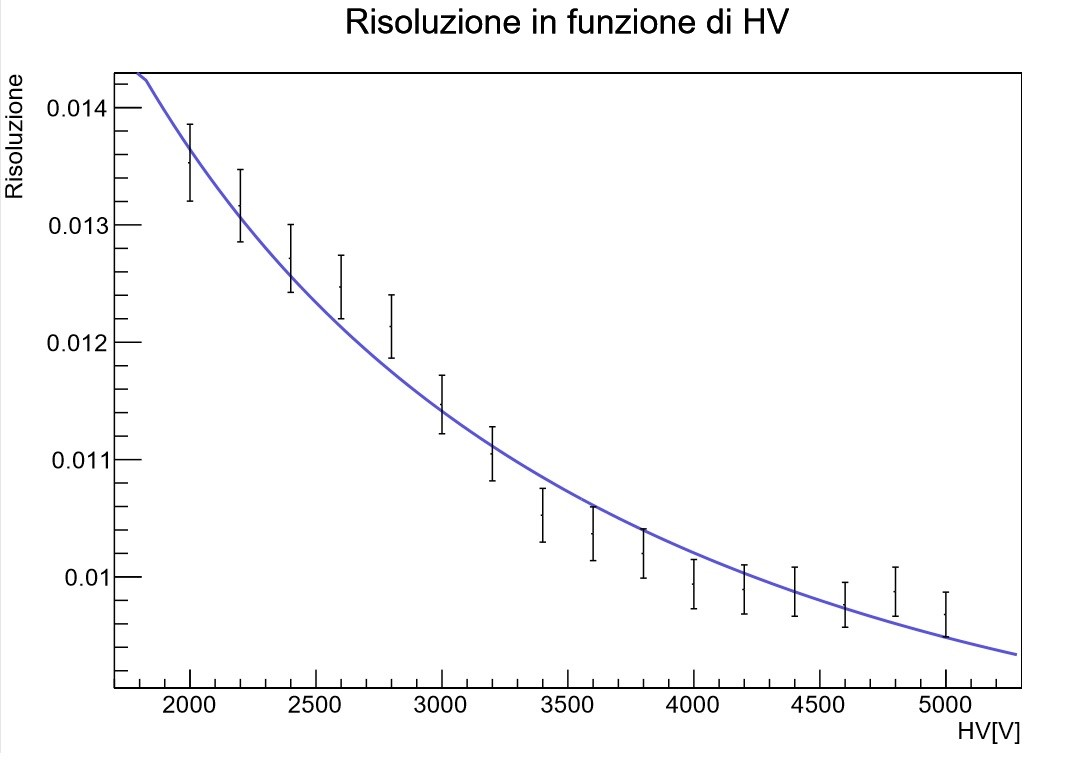
\includegraphics[scale=0.5]{grafici/risoluzionehv}
    \caption{Risoluzione in funzione della tensione di polarizzazione}
\end{figure}

\begin{figure}[!ht]
    \centering
    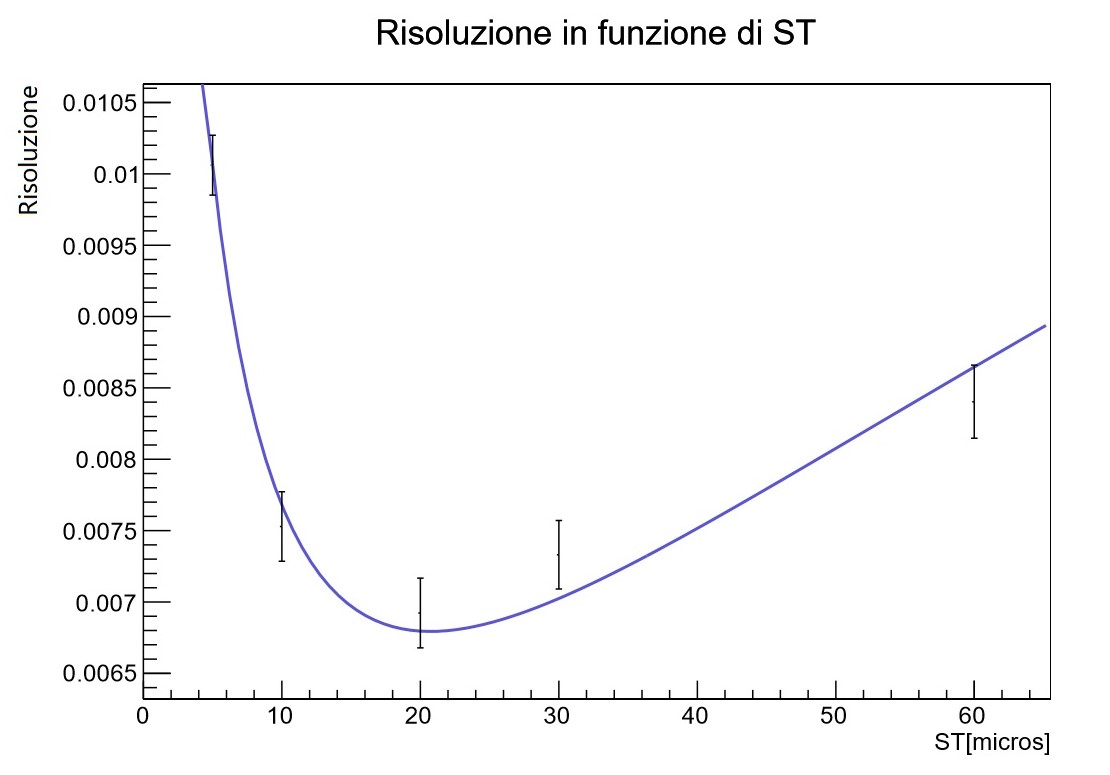
\includegraphics[scale=0.5]{grafici/risoluzionest}
    \caption{Risoluzione in funzione dello shaping time}
\end{figure}

\noindent I grafici sono stati interpolati con la seguente funzione: 
\begin{equation}
	R=\sqrt{\frac{\textrm{a}}{\textrm{x}}+\textrm{bx}}
\end{equation}
con x che indica in un caso la tensione e nell'altro lo shaping time.
\noindent I valori di $\chi^2$-ridotto e \textit{P-Value} mostrano come il modello teorico sia conforme ai dati a nostra disposizione.
\noindent Il nostro obiettivo era di ricavare i valori che minimizzassero la risoluzione. Nel caso della tensione di polarizzazione la risoluzione decresce, fino ad assestarsi intorno ad un valore costante oltre i 4000V, che pu\`o quindi essere preso come valore di riferimento. Nel caso dello shaping time la risoluzione ha un minimo in corrispondenza di uno shaping time di 2 $\mu$s, ed oltre quel valore torna a crescere, a causa del pile-up che diventa sempre pi\`u significativo. Sottolineaiamo che in questo caso non \`e stato inserito il valore riferito ad uno shaping time di 100 $\mu$s, non essendo stato possibile identificare con precisione la $\sigma$ di quel picco. Si precisa pertanto che a valori di quest'ultimo non si effettuano mai misure per via della presenza sempre pi\`u evidente del pile-up.
\subsection{Calibrazione in energia del rivelatore}

%%% CURVA DI CALIBRAZIONE CON Na, Co, Th %%%

\subsubsection{Curva di calibrazione}
Abbiamo a disposizione 3 sorgenti note: 22Na, 60Co e 228Th. Di queste 3 sorgenti andiamo a considerare gli spettri:

\begin{figure}[!h]
    \centering
    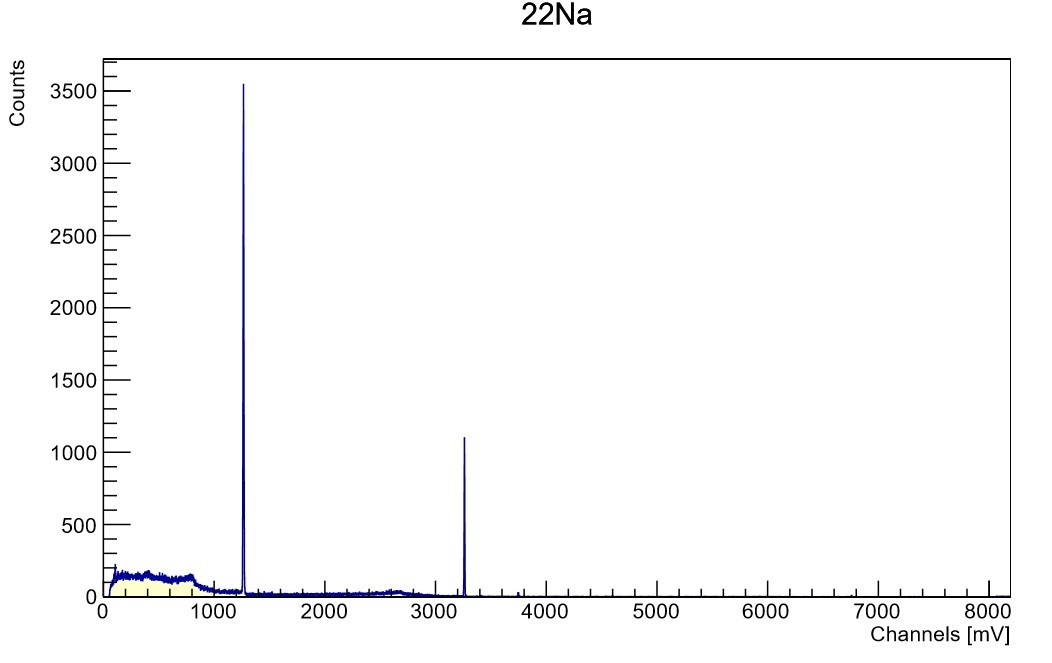
\includegraphics[scale=0.6]{grafici/sodiocompleto}
    \caption{Spettro 22Na}
\end{figure}
\newpage
\begin{figure}[!h]
    \centering
    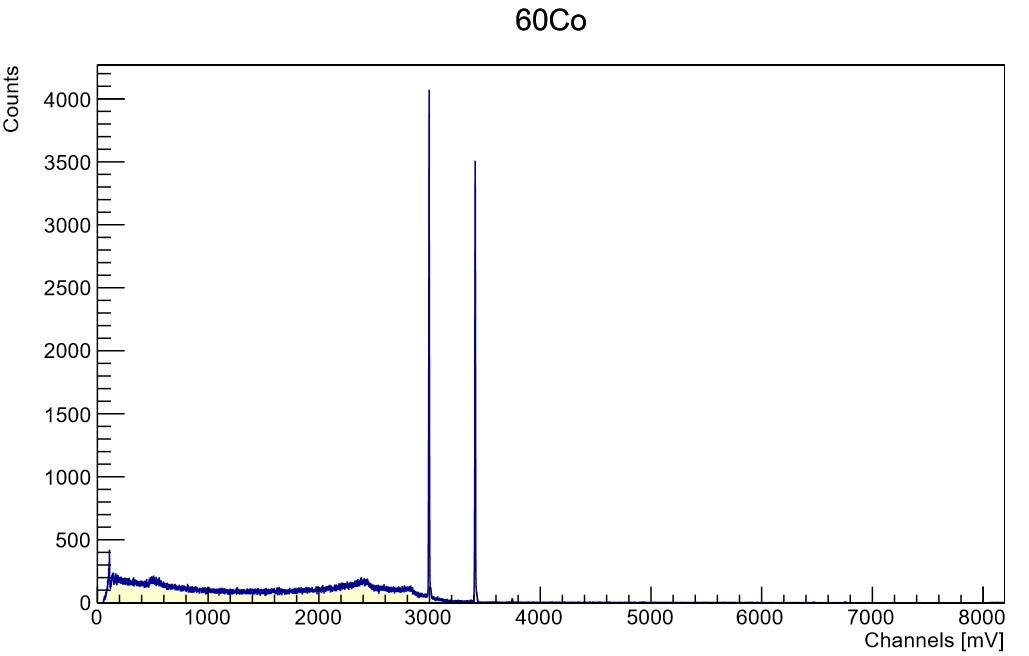
\includegraphics[scale=0.6]{grafici/cobaltocompleto}
    \caption{Spettro 60Co}
\end{figure}

\begin{figure}[!h]
    \centering
    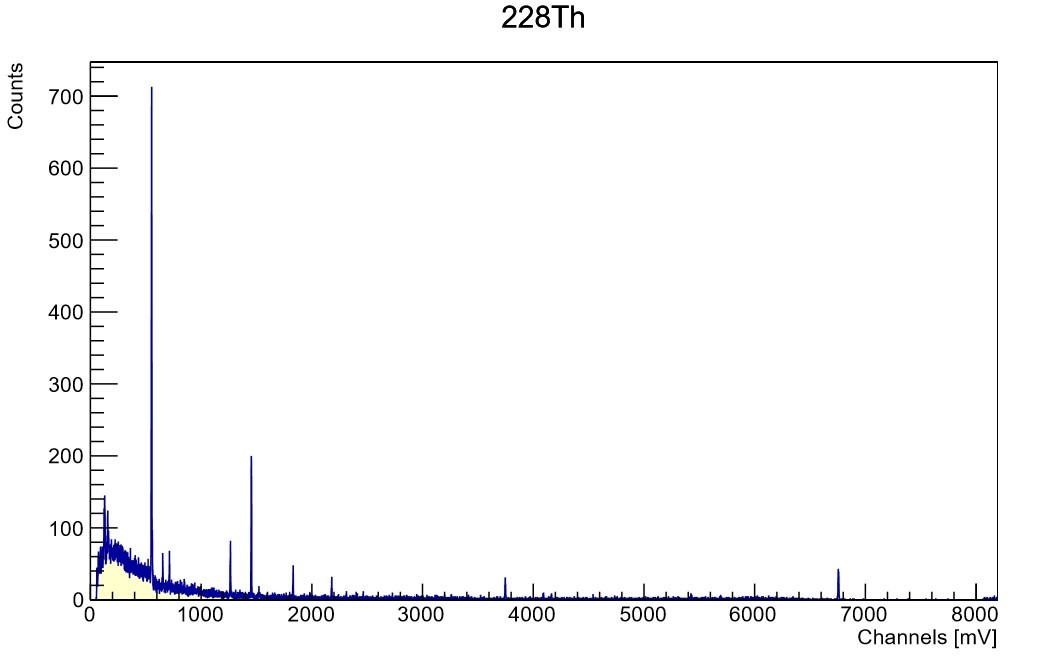
\includegraphics[scale=0.6]{grafici/toriocompleto}
    \caption{Spettro 228Th}
\end{figure}

\noindent Come fatto precedentemente, andiamo ad effettuare un ingrandimento su ognuno dei picchi per poterne ottenere posizione e sigma. Per quanto riguarda il sodio \`e stato considerato il secondo picco, in quanto il primo rappresenta il picco dovuto all'annichilazione del positrone a 511 KeV. Per il torio, abbiamo tenuto conto solo dei picchi pi\`u intensi e distinguibili. Di seguito riportiamo un esempio per ogni sorgente (i restanti sono in Appendice):

\begin{figure}[H]
    \centering
    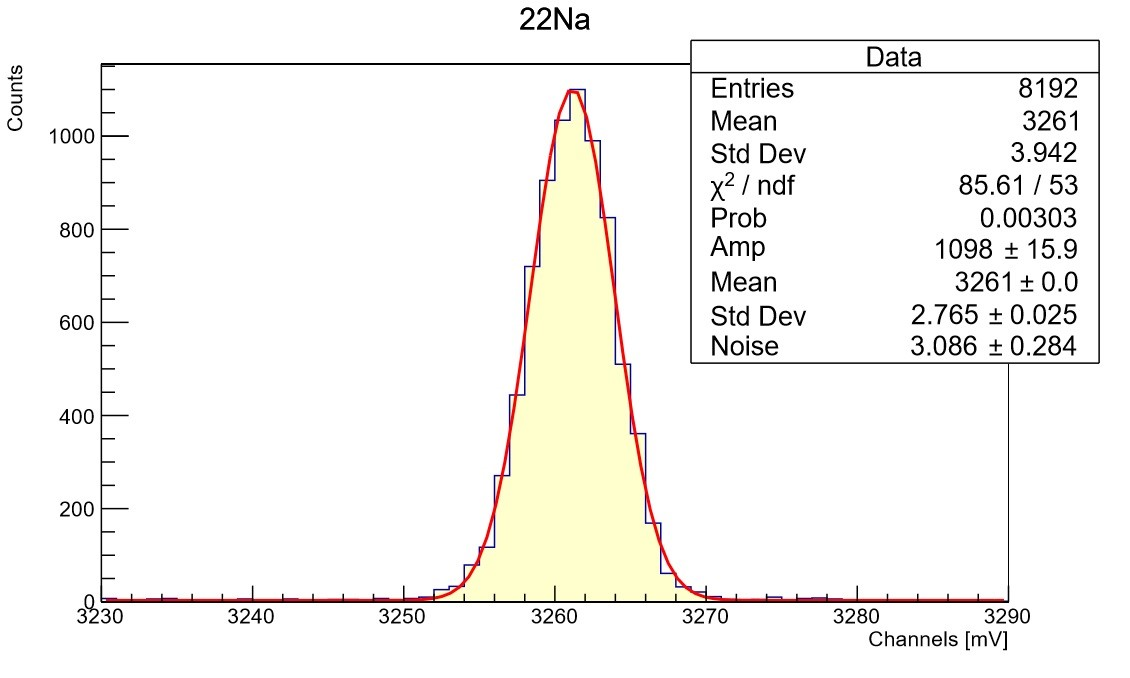
\includegraphics[scale=0.7]{grafici/piccoNa}
    \caption{Il picco del 22Na}
\end{figure}

\begin{figure}[H]
    \centering
    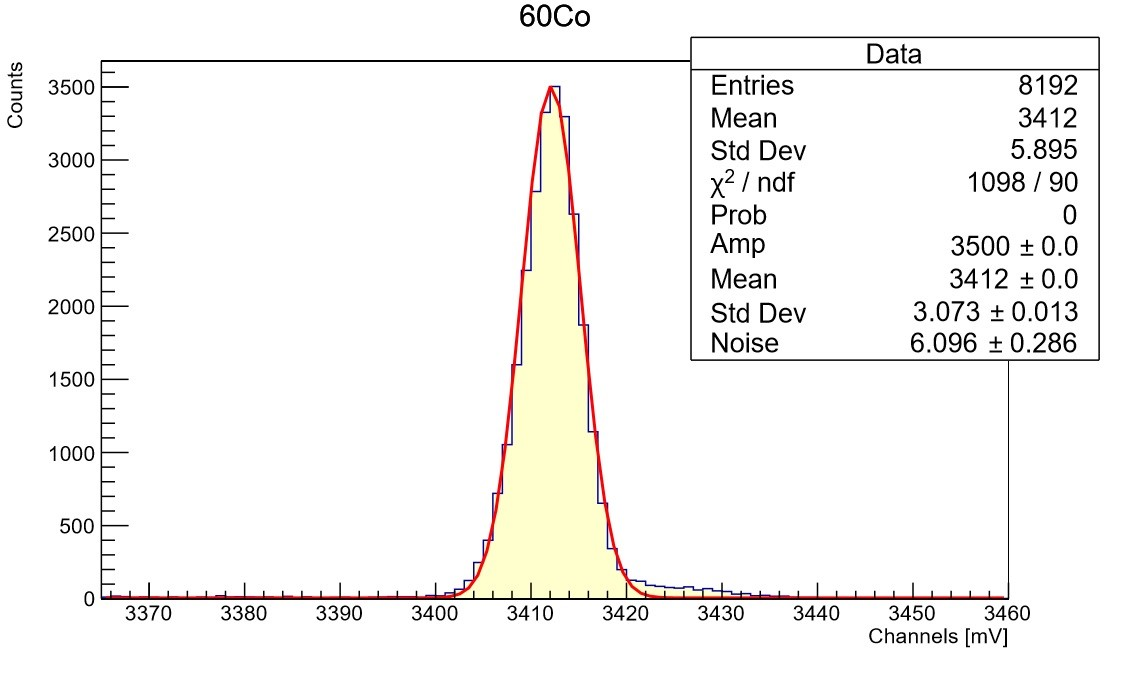
\includegraphics[scale=0.7]{grafici/piccoCo}
    \caption{Uno dei due picchi del 60Co}
\end{figure}

\begin{figure}[H]
    \centering
    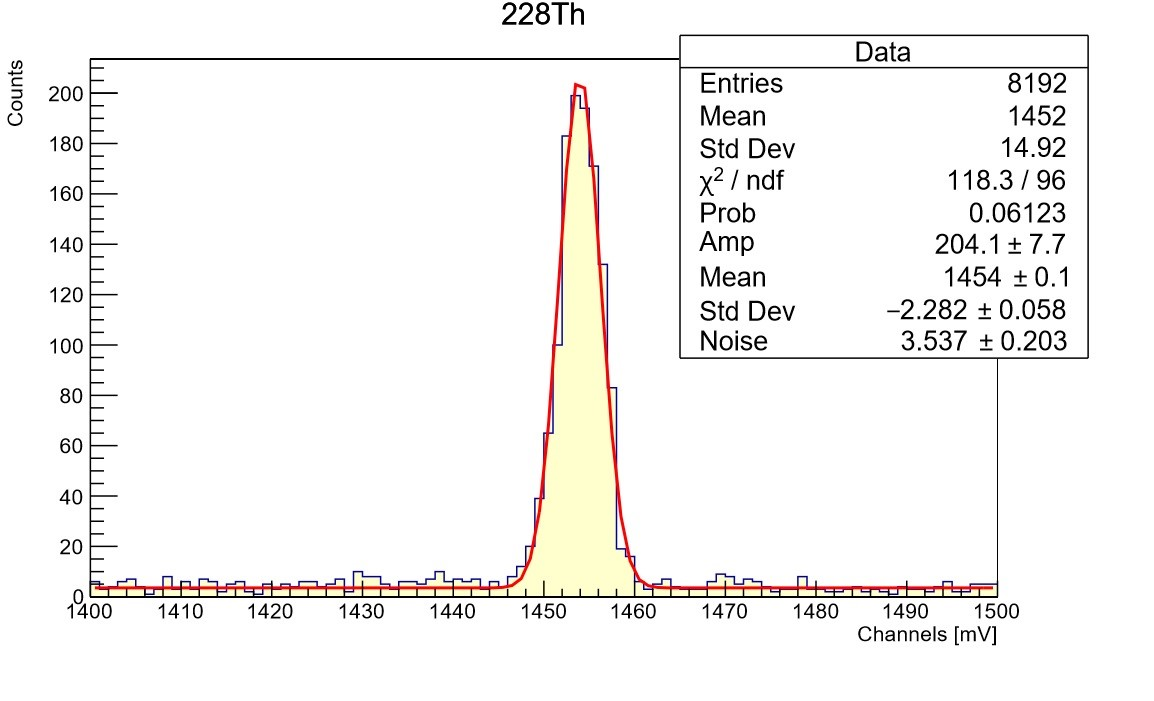
\includegraphics[scale=0.7]{grafici/piccoTh}
    \caption{Uno dei picchi del 228Th}
\end{figure}

\noindent Ognuno dei picchi individuati corrisponde ad una energia ben precisa. Nel seguente grafico viene riportata la curva di calibrazione, Energia vs. Canali:

\begin{figure}[H]
    \centering
    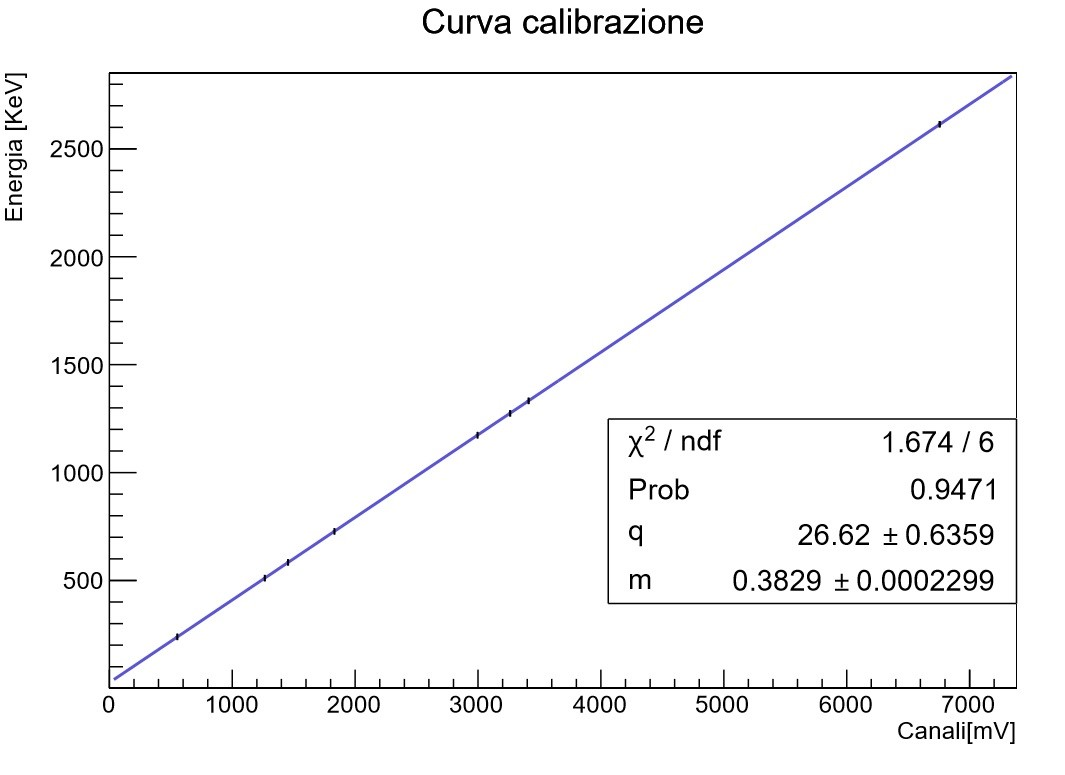
\includegraphics[scale=0.45]{grafici/rettacalibrazionesources}
    \caption{Energia vs. Canali}
\end{figure}

Il grafico \`e stato interpolato con la seguente funzione 
\begin{equation}
	\textrm{Energia} = m \times \textrm{Canale} + q
\end{equation}

ottenendo i seguenti parametri:

$$
	m=0.3829 \pm 2.3 \times 10^{-4}\, \unit{keV/mV}
$$
$$
	q=26.62 \pm 0.64\, \unit{keV}
$$

\noindent I valori di $\chi$\textsuperscript{2} ridotto e \textit{P-Value} riportati nel grafico mostrano come l'andamento lineare della relazione sia consistente. La relazione che intercorre fra energia e canali \`e dunque lineare.

%%% RISOLUZIONE CON Na, Co, Th %%%

\subsubsection{Risoluzione}
Vogliamo andare ad indagare la dipendenza della risoluzione in funzione dei valori di energia. La risoluzione \`e caratterizzata da 3 componenti: una statistica, che dipende linearmente dall'energia, una legata alla raccolta delle cariche, che dipende quadraticamente dall'energia, ed infine una legata al rumore elettronico, indipendente dall'energia. La risoluzione \`e stata calcolata con la relazione (1). Per quanto riguarda le incertezze si \`e tenuto conto della deviazione standard e dell'errore su quest'ultima. 

\begin{figure}[H]
    \centering
    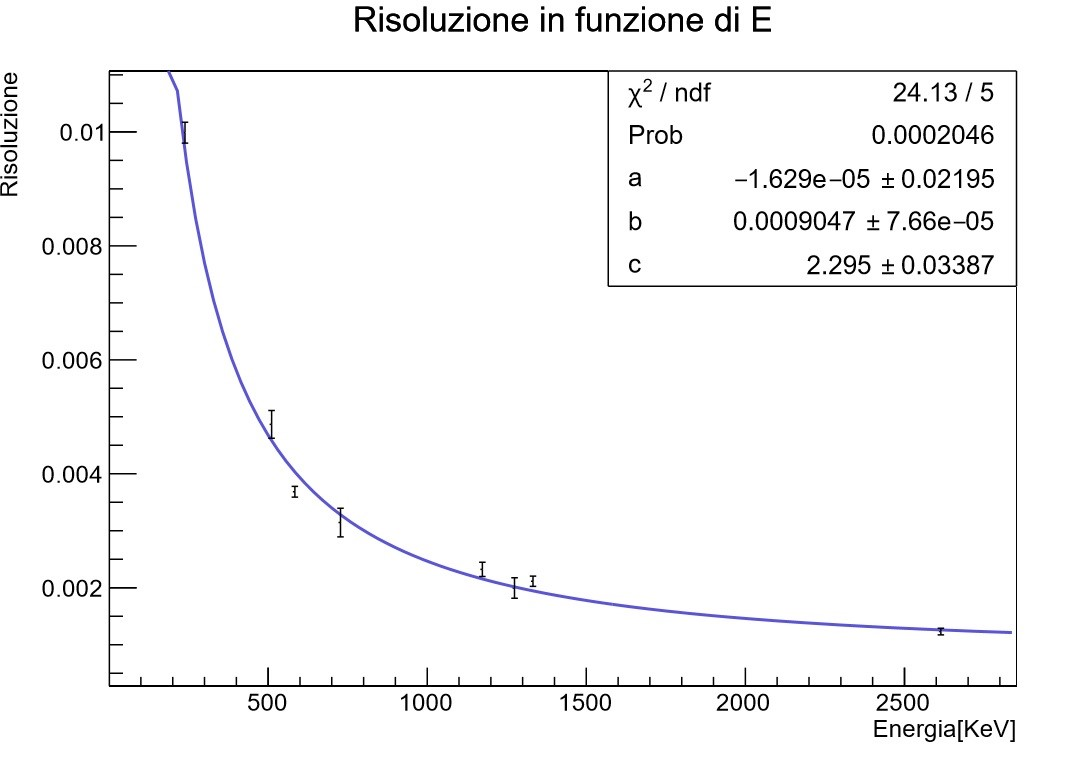
\includegraphics[scale=0.6]{grafici/risoluzionesources}
    \caption{Risoluzione in funzione di E}
\end{figure}

\noindent Per interpolare il grafico \`e stata utilizzata la relazione

\begin{equation}
	R=\sqrt{\frac{a^2}{E}+b^2+\frac{c^2}{E^2}}
\end{equation}

\noindent Con a, b e c che rispettivamente indicano i contributi legati alla statistica, alla raccolta delle cariche e al rumore. Sono riportati di seguito i valori:

$$
	a=1.63 \times 10{-5} \pm 2.20 \times 10^{-2} \unit{keV^{\frac{1}{2}}}
$$
$$
	b=9.01 \times 10^{-4} \pm 7.66 \times 10^{-5}
$$
$$
	c= 2.29 \pm 3.38 \times 10^{-2} \unit{keV}
$$

\noindent Dal valore dei parametri si nota come il parametro c sia diversi ordini di grandezza maggiore degli altri due, mostrando come il contributo principale alla risoluzione sia da attribuire alla componente legata al rumore elettronico.

%%% EFFICIENZA CON Na, Co, Th %%%

\subsubsection{Efficienza}
Per lo studio dell'efficienza assoluta sono stati considerati il numero di quanti totali emessi dalla sorgente, tenendo conto dell'attivit\`a della stessa e della durata della misura, ed il numero di conteggi riferito ad ogni picco. L'efficienza assoluta di picco \`e stata dunque calcolata con la seguente formula:

\begin{equation}
	\textrm{Efficienza}=\frac{\textrm{Conteggi picco}}{\textrm{Numero di eventi totali}}=\frac{\textrm{Conteggi picco}}{\textrm{Attivit\`a} \times \textrm{durata misura}}
\end{equation}

\noindent I valori ottenuti sono stati normalizzati per il Branching Ratio (B.R.) di ogni singolo decadimento, per rendere coerente il grafico. Il grafico viene riportato in scala logaritmica, e la funzione empirica utilizzata per interpolarlo \`e:

\begin{equation}
	\ln{\textrm{Efficienza}}=a + b\ln{\textrm{Energia}} + c\ln^{2}{\textrm{Energia}}
\end{equation}

\begin{figure}[H]
    \centering
    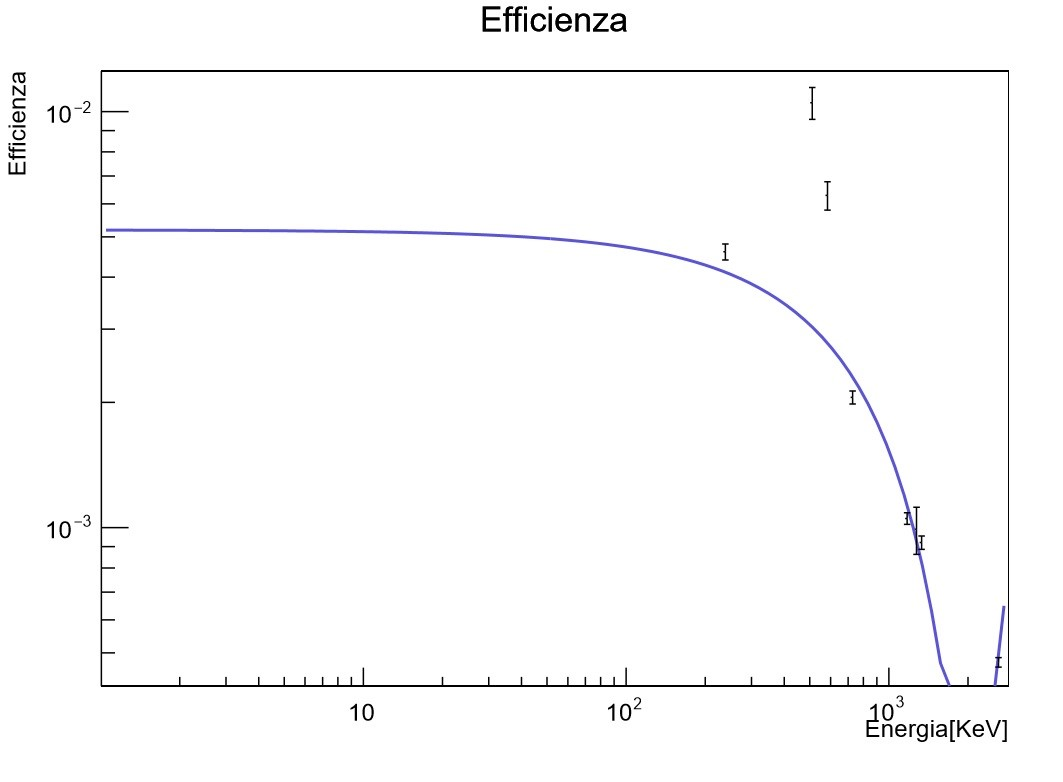
\includegraphics[scale=0.45]{grafici/efficienzasources}
    \caption{Efficienza in funzione di E}
\end{figure}

\noindent L'andamento dell'efficienza, come testimoniano i pessimi valori di $\chi^2$-ridotto e \textit{P-Value}, non \`e quello atteso. Alcuni punti si discostano dall'andamento che prevede l'efficienza assoluta del rivelatore diminuire all'aumentare dell'energia, non adattandosi al modello teorico. Non \`e stato possibile attribuire una incertezza precisa alle misure attraverso gli strumenti di ROOT, ed anche questo ha contribuito alla non riuscita della stima dell'efficienza del rivelatore.

\section{Parte 2}

%%% STRUMENTAZIONE PARTE 2 %%%

\subsection{Strumentazione}
\begin{itemize}
\item Crate NIM Ortec Modle 4001A
\item Rivelatore coassiale HPGe (Silena)
\item Generatore HV Ortec Model 659 per tensione di polarizzazione
\item Amplificatore Ortec Model 570
\item ADC/MCA Ortec 920E
\item Sorgente multigamma
\item Sorgente ignota
\end{itemize}
\subsection{Calibrazione in energia del rivelatore}

%%% CURVA DI CALIBRAZIONE CON MULTIGAMMA %%%
 
\subsubsection{Curva di calibrazione}
Il segnale \`e acquisito, come della parte 1 dell'esperienza, da una catena di lettura classica, con i componenti integrati nello stesso modo. Come prima cosa, \`e nostra necessit\`a costruire una curva di calibrazione Energia vs. Canali. Allo scopo viene utilizzata una sorgente multigamma: la sorgente \`e composta da diversi radionuclidi, ognuno con la sua attivit\`a ed una energia tabulata per i gamma emessi. Vengono calcolate, per ogni radionuclide, le attività riferite al giorno in cui \`e stata effettuata la misura. Viene utilizzata la formula del decadimento:

\begin{equation}
	A(t)=A_{0}e^{-t/\tau}
\end{equation}

\noindent dove $A_{0}$ rappresenta l'attivit\`a al tempo 0 del radionuclide, indicata sulla scheda di certificazione, e $\tau$ \`e una caratteristica legata al tempo di dimezzamento del radionuclide. Al giorno della misura, risultano attivi i seguenti radionuclidi:

\begin{center}
    \begin{tabular}{cccc}
        \toprule
        Nuclide & $A_{0}$[Bq] & $\bar{A}$[Bq] & $E_{\gamma}$[MeV]\\
        \midrule
         241-Am & $3.45 \times 10^3$ & 3410 & 0.060\\
	  109-Cd & $1.58 \times 10^4$ & 322 & 0.088\\
	  137-Cs & $2.72 \times 10^3$ & 2300 & 0.662\\
	  60-Co & $3.21 \times 10^3$ & 1284 & 1.173\\
	  60-Co & $3.21 \times 10^3$ & 1284 & 1.333\\
        \bottomrule
    \end{tabular}\\
\end{center}

\noindent Con $\bar{A}$ si \`e indicata l'attivit\`a al momento della misura.
\noindent A questo punto, viene analizzato lo spettro della sorgente multigamma utilizzata:

\begin{figure}[H]
    \centering
    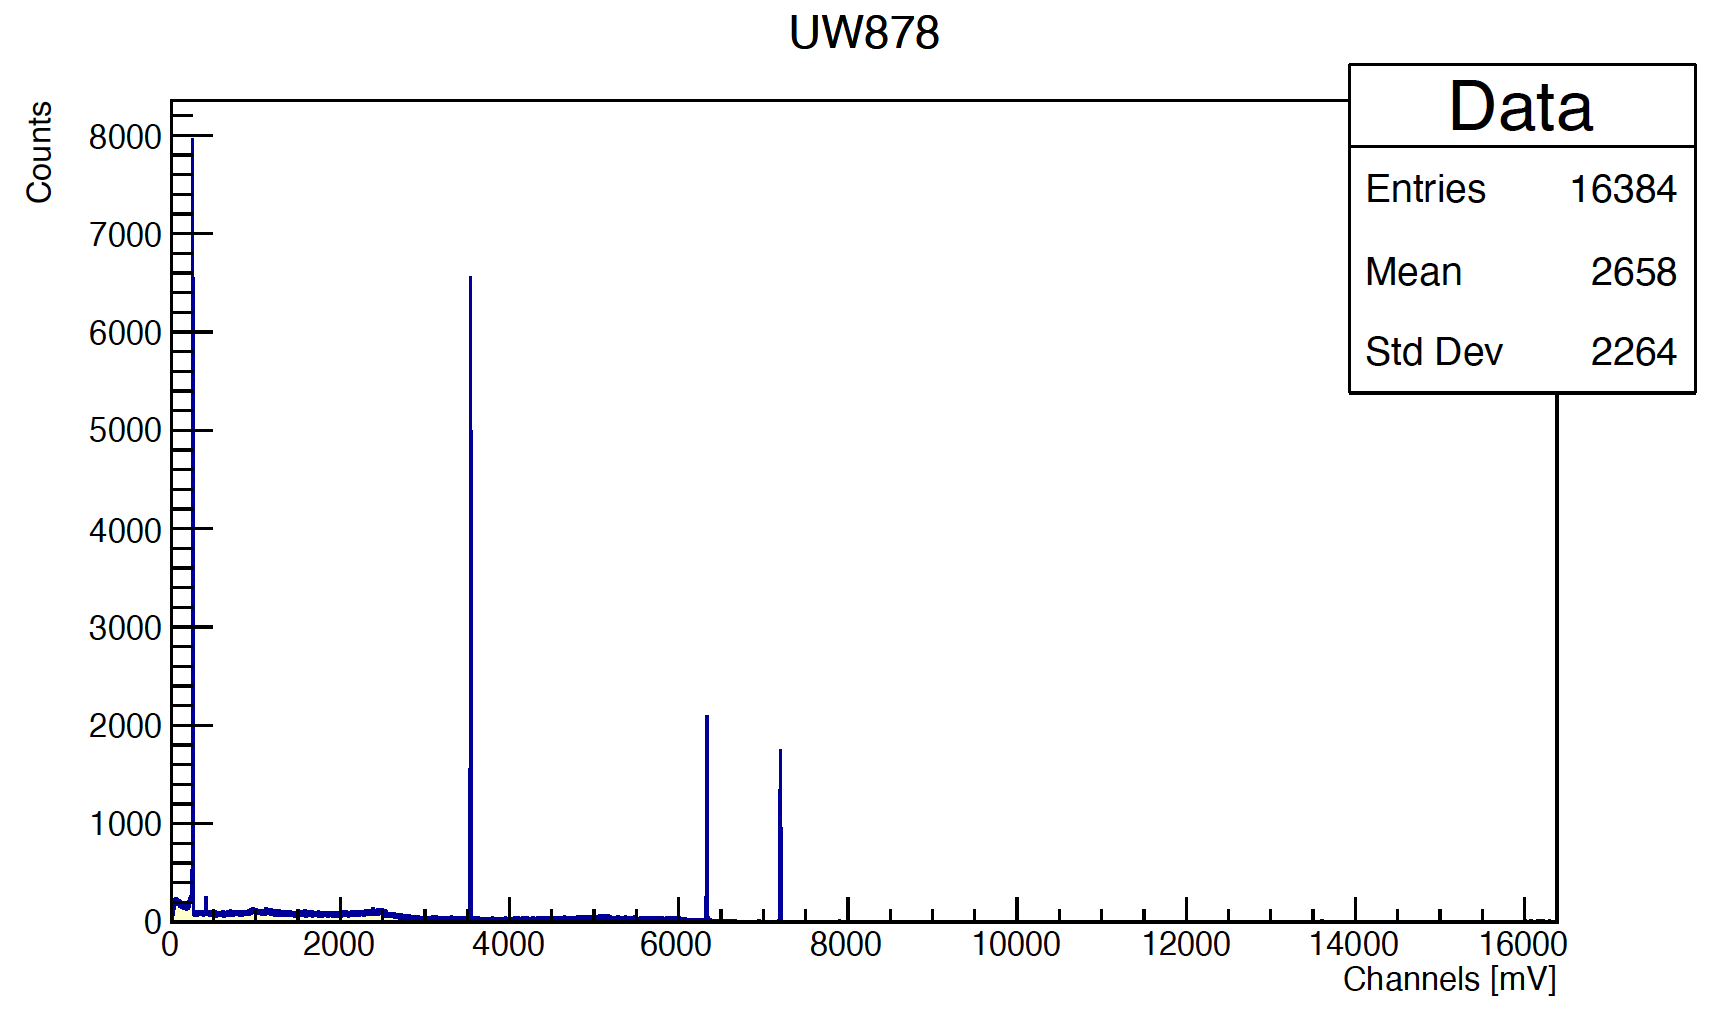
\includegraphics[scale=0.45]{grafici/uw878}
    \caption{Spettro sorgente multigamma}
\end{figure}

\noindent Analogamente alla parte 1, viene effettuato un ingrandimento per individuare la posizione del picco e la relativa $\sigma$:

\begin{figure}[H]
    \centering
    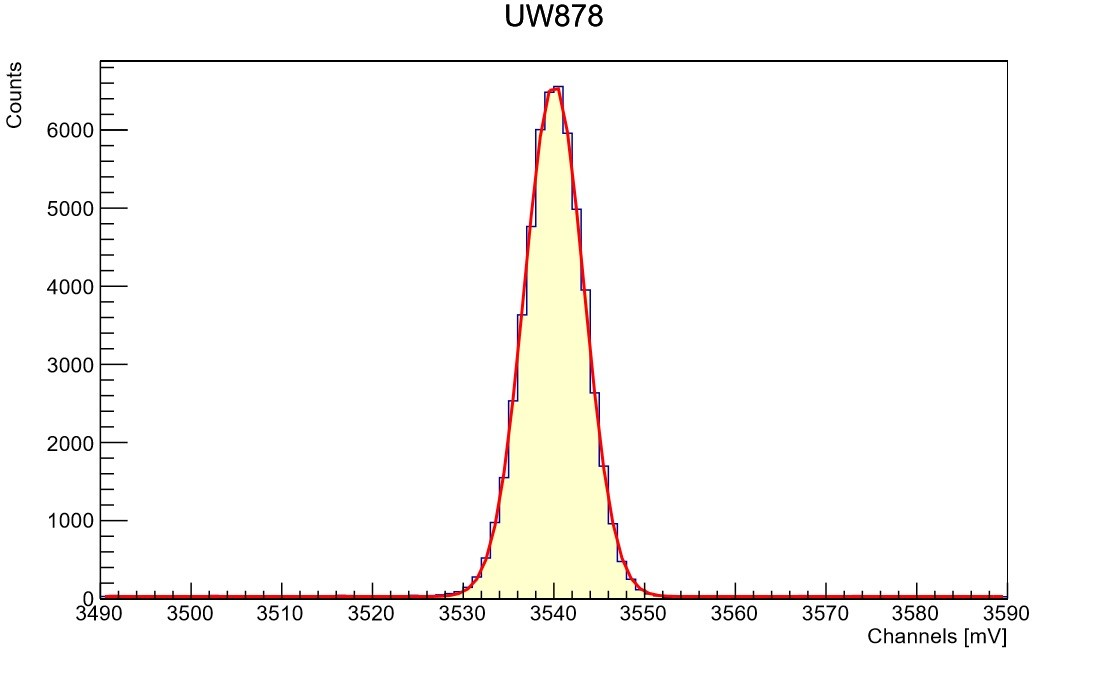
\includegraphics[scale=0.6]{grafici/piccouw878}
    \caption{Uno dei picchi individuati}
\end{figure}

\noindent Vengono individuati 6 picchi, uno dei quali corrisponde ad una energia di 2505 KeV. L'andamento della curva di calibrazione \`e il seguente:

\begin{figure}[H]
    \centering
    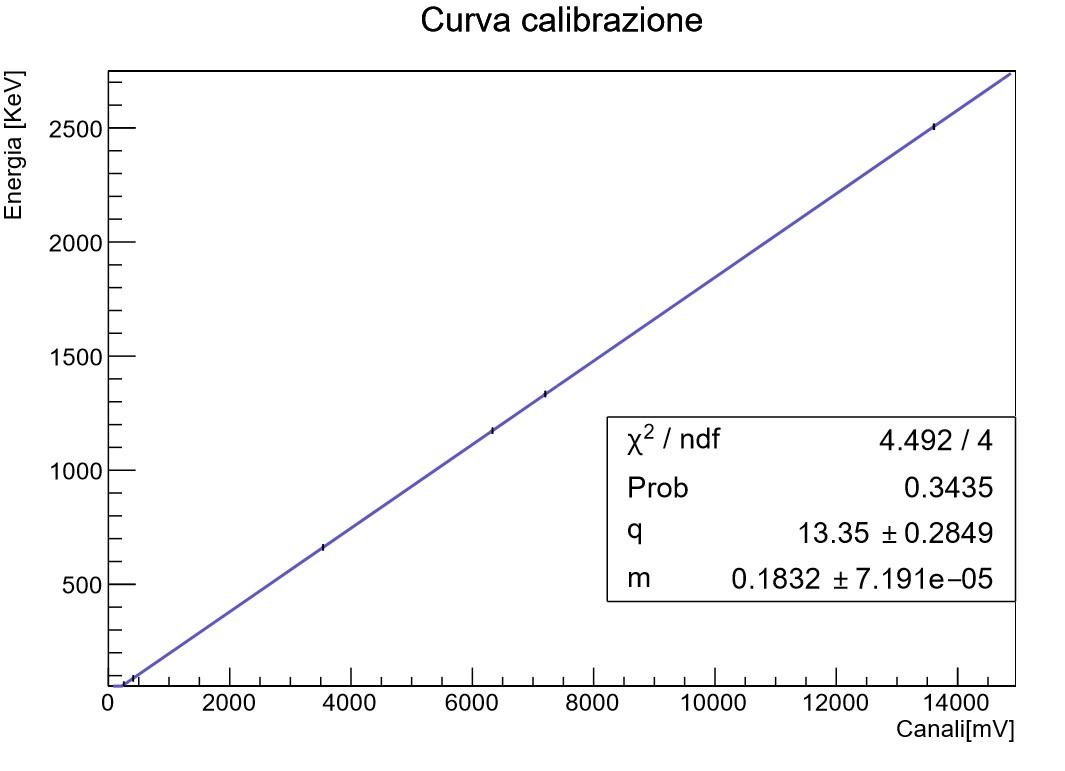
\includegraphics[scale=0.45]{grafici/rettacalibrazionemultigamma}
    \caption{Energia vs. Canali}
\end{figure}

\noindent Si sfrutta la relazione (3) per interpolare il grafico. Si ottengono i seguenti parametri:

$$
	m=0.18 \pm 7.19 \times 10^{-5}\, \unit{kev/mV}
$$
$$
	q=13.35 \pm 0.28\, \unit{keV}
$$
L'andamento della curva \`e chiaramente lineare giustificato anche dal valore di $\chi^2$-ridotto prossimo a 1. Il picco presente a 2505 KeV, non previsto fra quelli attesi nella misura, \`e attribuibile al fatto che in alcuni casi la risoluzione temporale del rivelatore non \`e sufficientemente alta da distinguere in maniera precisa due eventi successivi, come sono in questo caso l'emissione dei due gamma della sorgente di 60-Co. In questi casi il rivelatore legge i due eventi come un evento singolo, registrando un'energia pari alla somma dei due gamma del cobalto, circa pari a 2500 KeV.

%%% RISOLUZIONE CON MULTIGAMMA %%%

\subsubsection{Risoluzione}
Analogamente alla parte 1, utilizziamo la relazione (1) per calcolare la risoluzione di ogni picco. Utilizziamo invece la relazione (4) per interpolare il grafico ottenuto:

\begin{figure}[H]
    \centering
    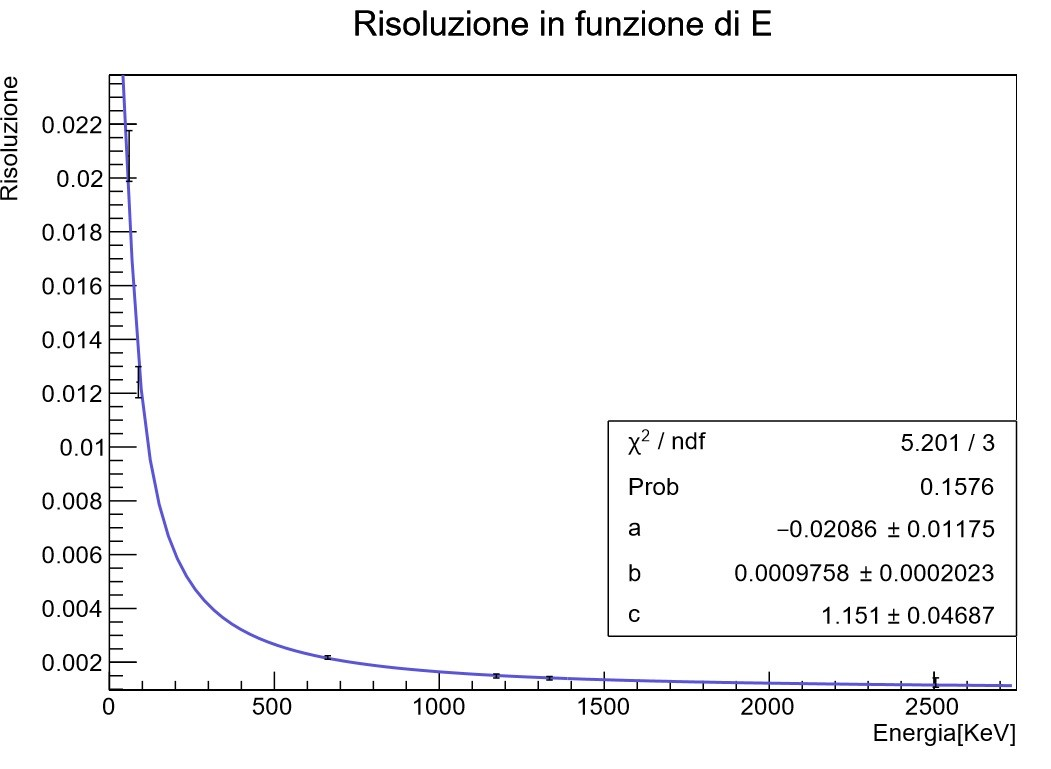
\includegraphics[scale=0.45]{grafici/risoluzionemultigamma}
    \caption{Risoluzione in funzione di E}
\end{figure}

\noindent Con a, b e c che rispettivamente indicano i contributi legati alla statistica, alla raccolta delle cariche e al rumore. Sono riportati di seguito i valori:

$$
	a=2.08 \times 10^{-2} \pm 1.17 \times 10^{-2} \unit{keV^{\frac{1}{2}}}
$$
$$
	b=9.76 \times 10^{-4} \pm 2.02 \times 10^{-4}
$$
$$
	c= 1.15 \pm 4.69 \times 10^{-2} \unit{keV}
$$

\noindent Anche in questo caso il contributo pi\`u rilevante \`e quello legato al rumore elettronico.

%%% EFFICIENZA CON MULTIGAMMA %%%

\subsubsection{Efficienza}
Sono state utilizzate la relazione (5) per il calcolo dell'efficienza assoluta di ogni picco, normalizzando anche in questo caso per il Branching Ratio, e la relazione (6) per interpolare il grafico:

\begin{figure}[H]
    \centering
    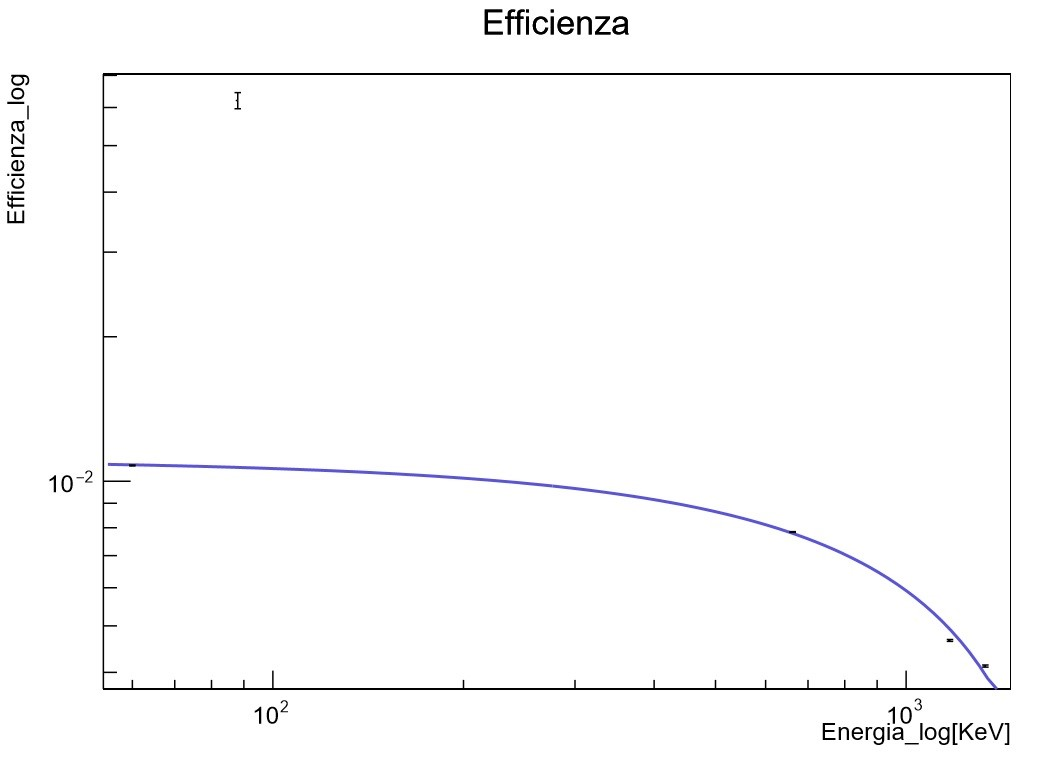
\includegraphics[scale=0.45]{grafici/efficienzamultigamma}
    \caption{Efficienza in funzione di E}
\end{figure}

\noindent Anche in questo caso si pu\`o notare dai valori di $\chi^2$-ridotto e \textit{P-Value} come l'andamento non sia quello atteso, nonostante solo uno dei punti considerati, quello corrispondente al picco relativo al 109-Cd, si discosti in maniera importante da esso. Risulta pi\`u evidente rispetto alla parte 1 l'andamento decrescente dell'efficienza all'aumentare dell'energia, suppur anche in questo caso non sia stato possibile determinare con precisione una incertezza per le varie misure.

\subsection{Sorgente ignota}

%%% INDIVIDUAZIONE SORGENTE IGNOTA %%%

\subsubsection{Riconoscimento}
A nostra disposizione abbiamo una acquisizione di dati senza sorgente ed una con la sorgente. In questo modo, sottraendo i conteggi senza sorgente per ogni canale a quelli con la sorgente, siamo in grado di ottenere i contributi effettivi della sorgente stessa. Andiamo ad ottenere il seguente spettro:

\begin{figure}[H]
    \centering
    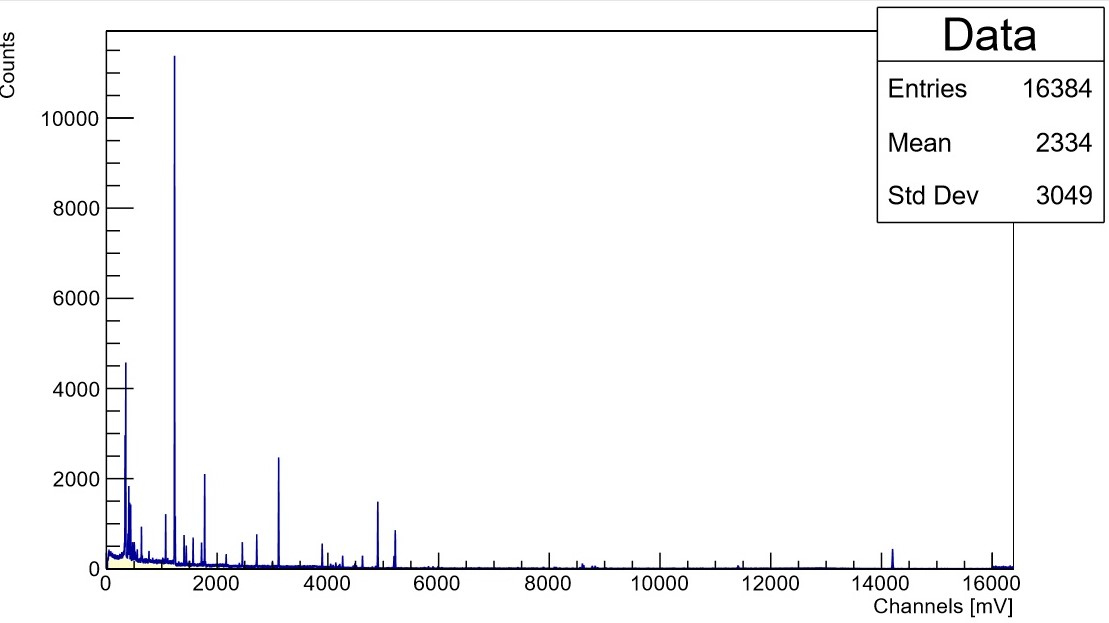
\includegraphics[scale=0.6]{grafici/sorgenteignota}
    \caption{Spettro sorgente ignota}
\end{figure}

\noindent Il numero di picchi \`e molto elevato: andiamo ad analizzare principalmente quelli pi\`u intensi ed evidenti. Come nelle parti precedenti, la posizione del picco con la relativa $\sigma$ vengono ricavate dal grafico ingrandito nella regione di interesse, interpolando con una gaussiana e un polinomio di grado zero che tenga conto del rumore. Attraverso i canali individuati risaliamo alle energie corrispondenti con i relativi errori (propagazione degli errori), utilizzando la curva di calibrazione ricavata nella sezione 3.2.1. Nella seguente tabella indichiamo nell'ultima colonna il nuclide responsabile dell'emissione del gamma di quella precisa energia:

\begin{center}
    \begin{tabular}{c c c c c}
        \toprule
        Canale [mV] & $\sigma_{\textrm{Canale}}$ [mV] & Energia [keV] & $\sigma_{\textrm{Energia}}$ [keV] & Nuclide\\
        \midrule
	  338 & 3 & 75.20 & 0.54 & 228-Th\\
	  350 & 3 & 77.45 & 0.54 & 228-Ac\\
	  390 & 3 & 84.78 & 0.63 & 228-Th\\
	  633 & 3 & 129.39 & 0.53 & 228-Ac\\
	  1232 & 3 & 239.05 & 0.57 & 212-Pb\\
	  1244 & 3 & 241.25 & 0.54 & 224-Ra\\
	  1404 & 3 & 270.56 & 0.58 & 228-Ac\\
	  1443 & 3 & 277.71 & 0.63 & 208-Tl\\
	  1567 & 3 & 300.42 & 0.60 & 212-Pb\\
	  1775 & 3 & 338.53 & 0.60 & 228-Ac\\
	  3111 & 3 & 583.29 & 0.67 & 208-Tl\\
	  4902 & 4 & 911.40 & 0.75 & 228-Ac\\
	  5195 & 4 & 965.07 & 0.77 & 228-Ac\\
	  5218 & 4 & 969.29 & 0.77 & 228-Ac\\
	  14200 & 6 & 2614.79 & 1.13 & 208-Tl\\
        \bottomrule
    \end{tabular}\\
\end{center}

\noindent Tutti i nuclidi individuati fanno parte della catena radioattiva del torio. Considerando che la sorgente utilizzata non pu\`o avere un tempo di dimezzamento troppo breve, altrimenti la sorgente si esaurirebbe velocemente, \`e ipotizzabile che la sorgente in questione sia del 228-Ra.

%%% RISOLUZIONE SORGENTE IGNOTA%%%

\subsubsection{Risoluzione}

Anche in questo caso andiamo a calcolare l'andamento della risoluzione del rivelatore in funzione dell'energia, usando la relazione (1) per calcolarla e la relazione (4) per interpolare il grafico:

\begin{figure}[H]
    \centering
    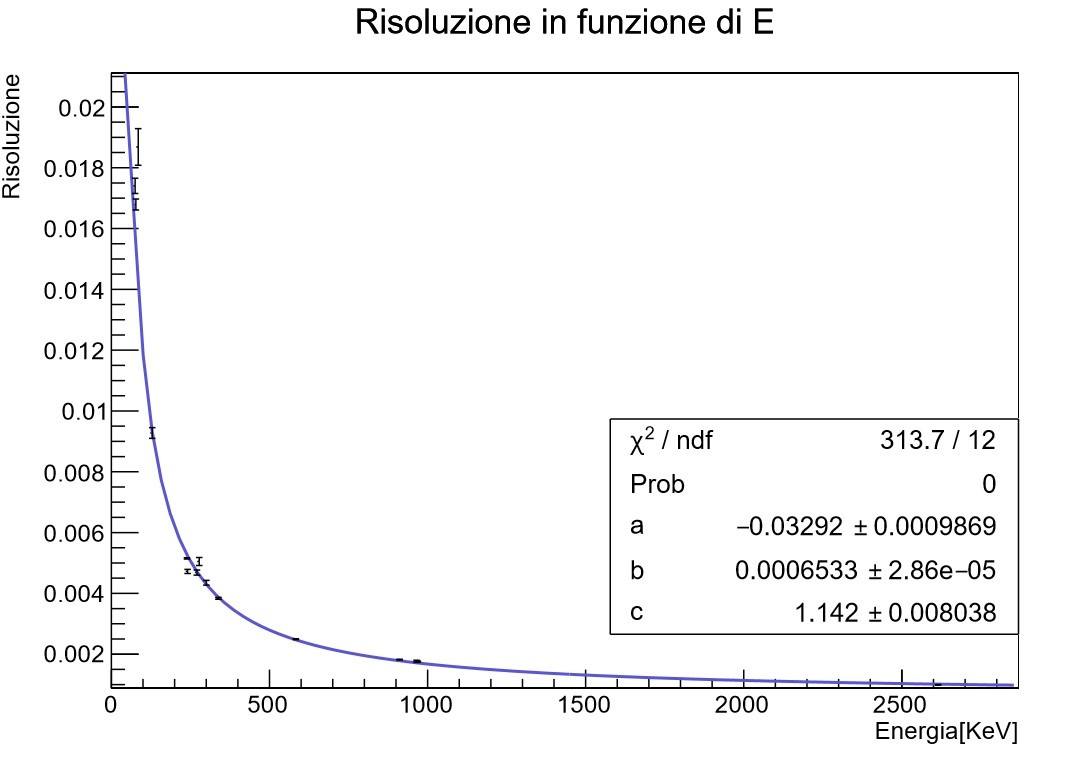
\includegraphics[scale=0.45]{grafici/risoluzioneignota}
    \caption{Risoluzione in funzione di E}
\end{figure}

\noindent Con a, b e c che rispettivamente indicano i contributi legati alla statistica, alla raccolta delle cariche e al rumore. Sono riportati di seguito i valori:

$$
	a=3.29 \times 10^{-2} \pm 9.87 \times 10^{-4} \unit{keV^{\frac{1}{2}}}
$$
$$
	b=6.53 \times 10^{-4} \pm 2.86 \times 10^{-5}
$$
$$
	c= 1.14 \pm 8.03 \times 10^{-3} \unit{keV}
$$

%%% DETERMINAZIONE FATTORE DI FANO %%%

\subsubsection{Determinazione del fattore di Fano}

Nella relazione (4) abbiamo indicato come il coefficiente a del nostro modello fosse relativo alla componente statistica della risoluzione. Pi\`u precisamente, si può definire:
$$
	a=\sqrt{2.35 \times F \times w}
$$

\noindent $F$ rappresenta il fattore di Fano, un coefficiente che nel calcolo tiene conto della statistica poissoniana, mentre $w$ rappresenta l'energia necessaria per produrre una coppia elettrone-lacuna nel materiale. Nel germanio il valore di $w$ \`e di 2.96 eV.

$$
	F=\frac{a^2}{2.35 \times w}
$$

\noindent Il valore del fattore di Fano calcolato \`e dunque 0.156 $\pm$ 0.009. Il cui errore è sempre ricavato per propagazione degli errori.

%%% APPENDICE %%%

\section{Appendice}
\subsection{High Voltage}
\begin{figure}[H]
    \centering
    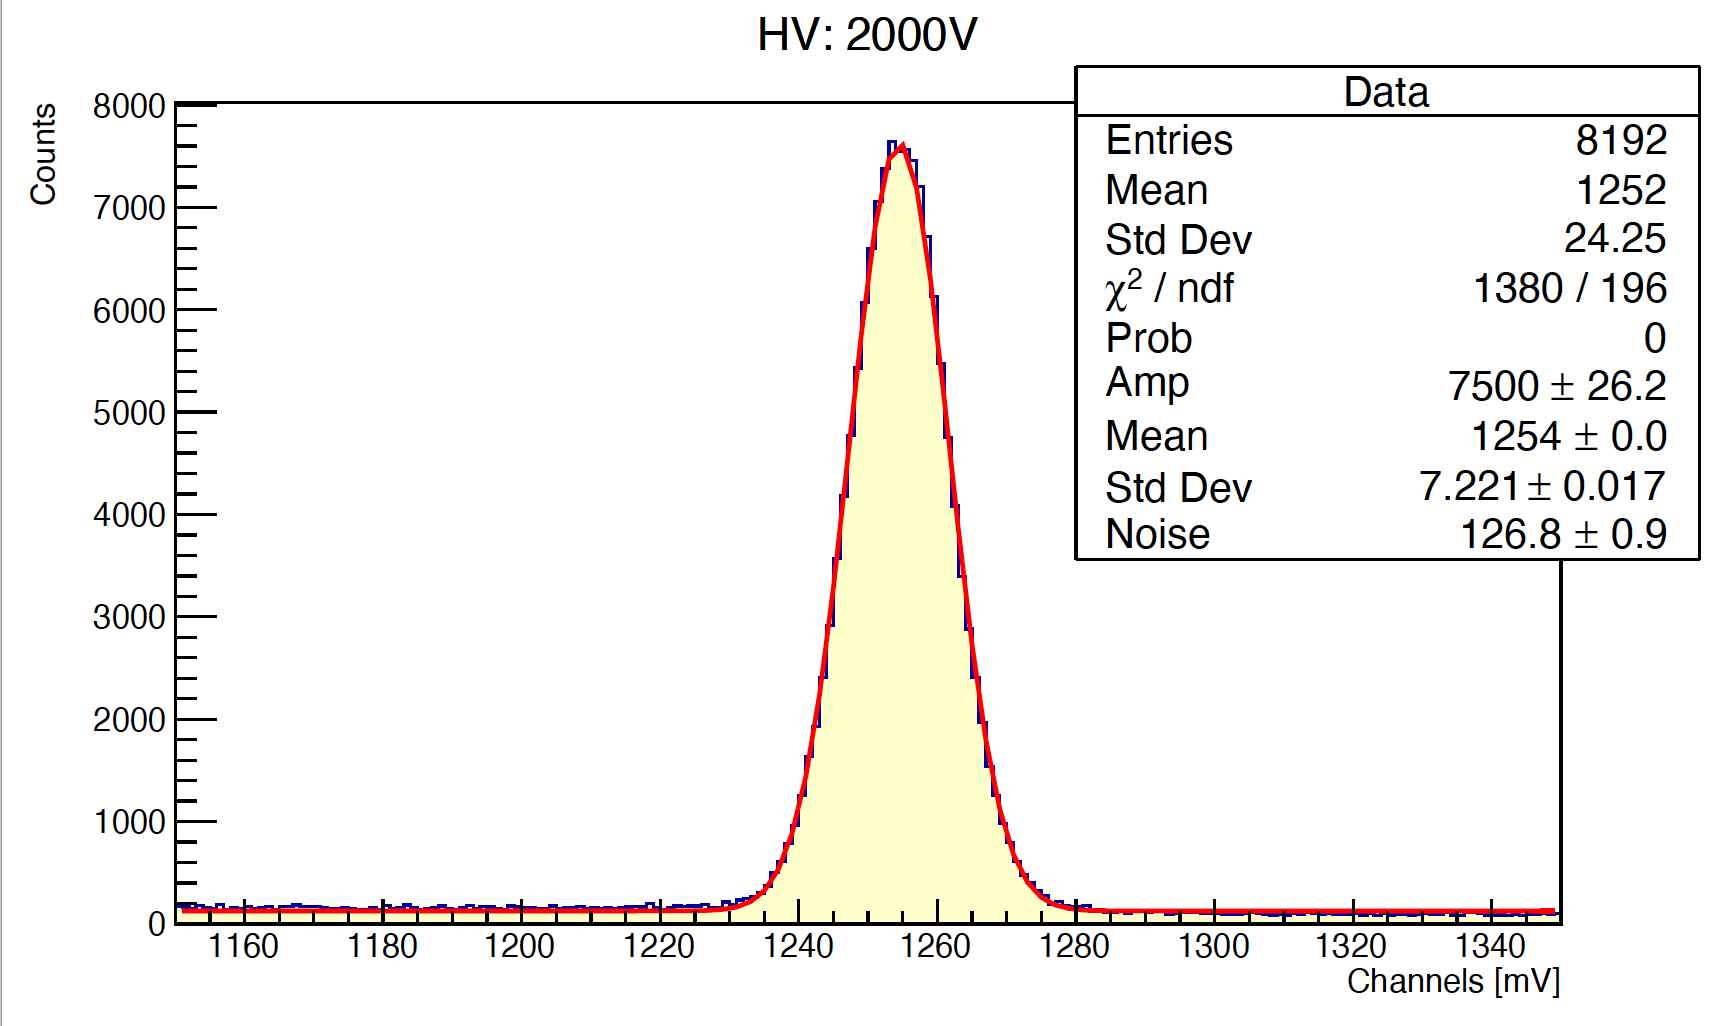
\includegraphics[scale=0.45]{appendice/2000}
\end{figure}
\begin{figure}[H]
    \centering
    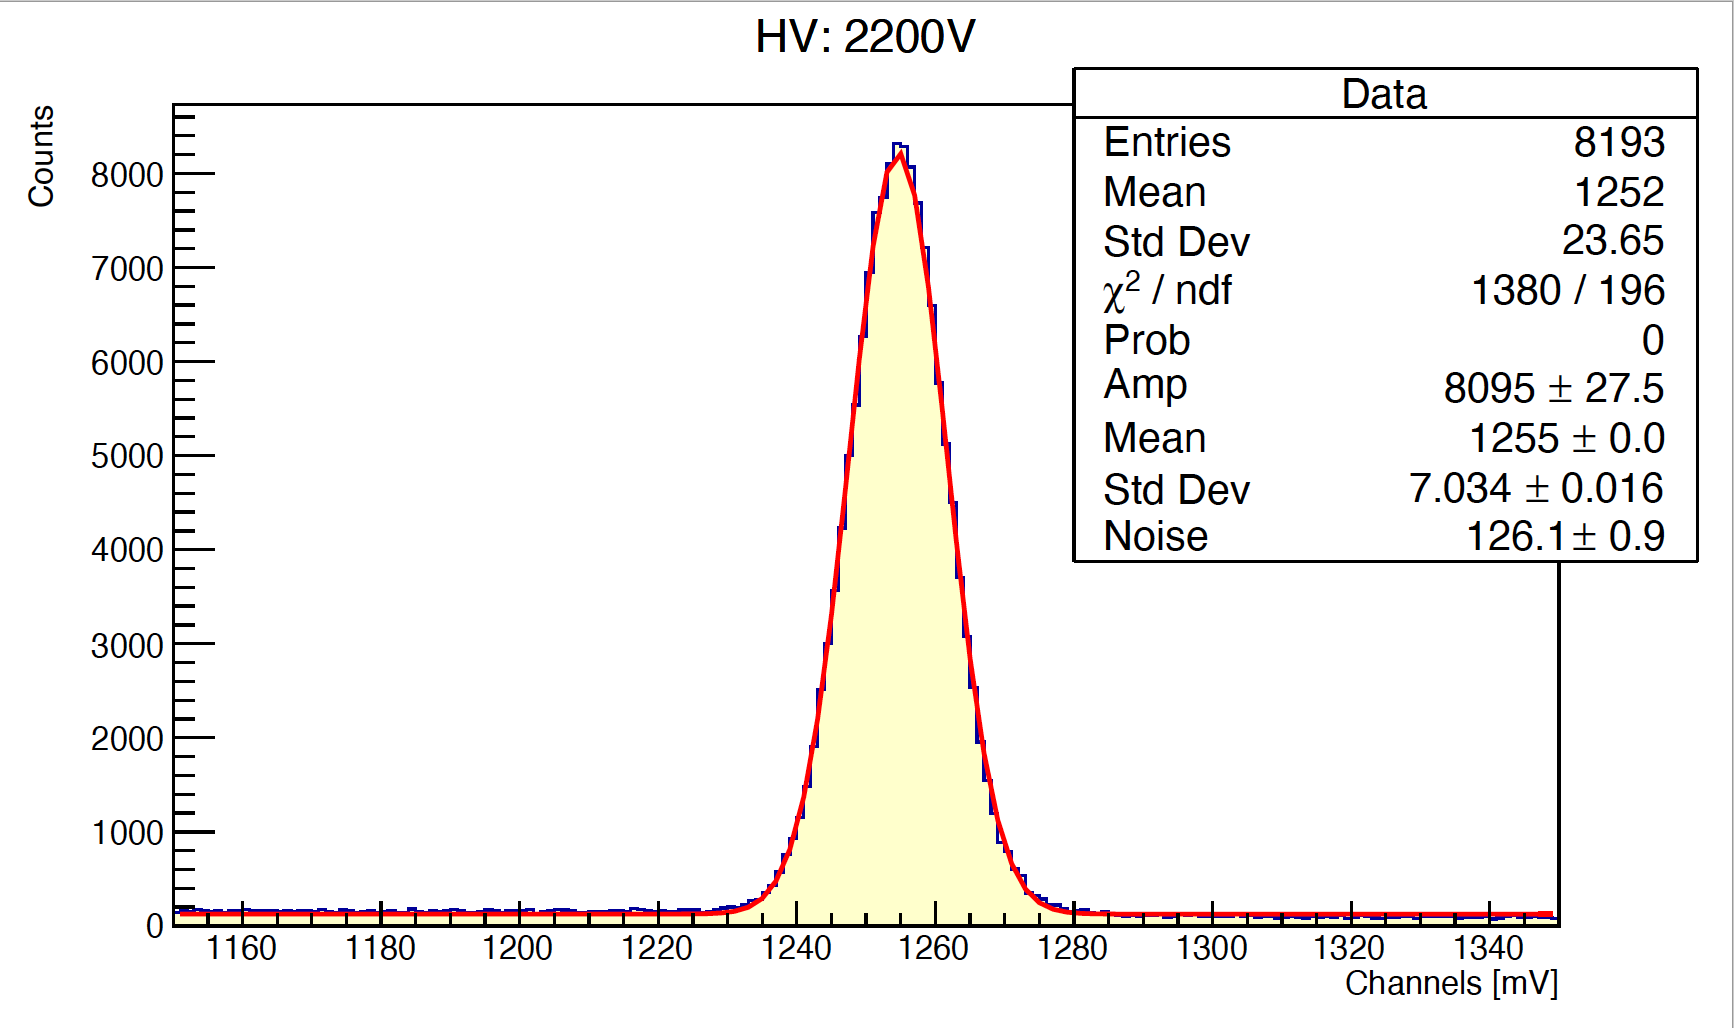
\includegraphics[scale=0.45]{appendice/2200}
\end{figure}
\begin{figure}[H]
    \centering
    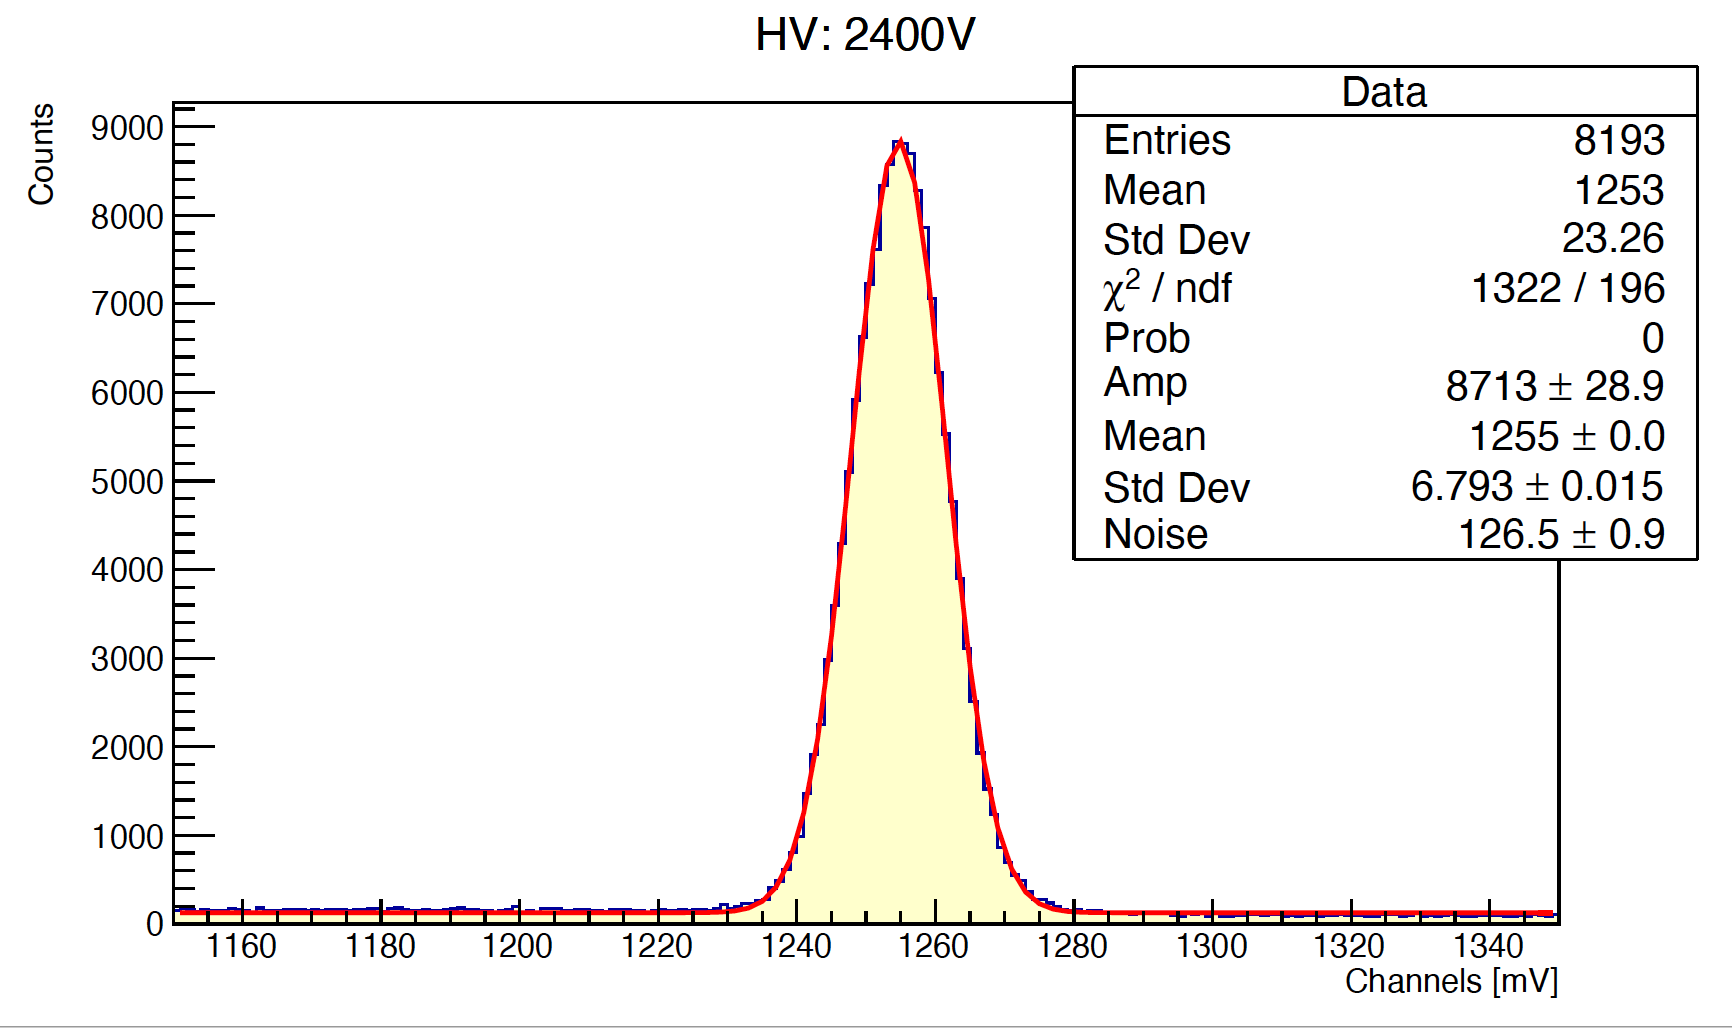
\includegraphics[scale=0.45]{appendice/2400}
\end{figure}
\begin{figure}[H]
    \centering
    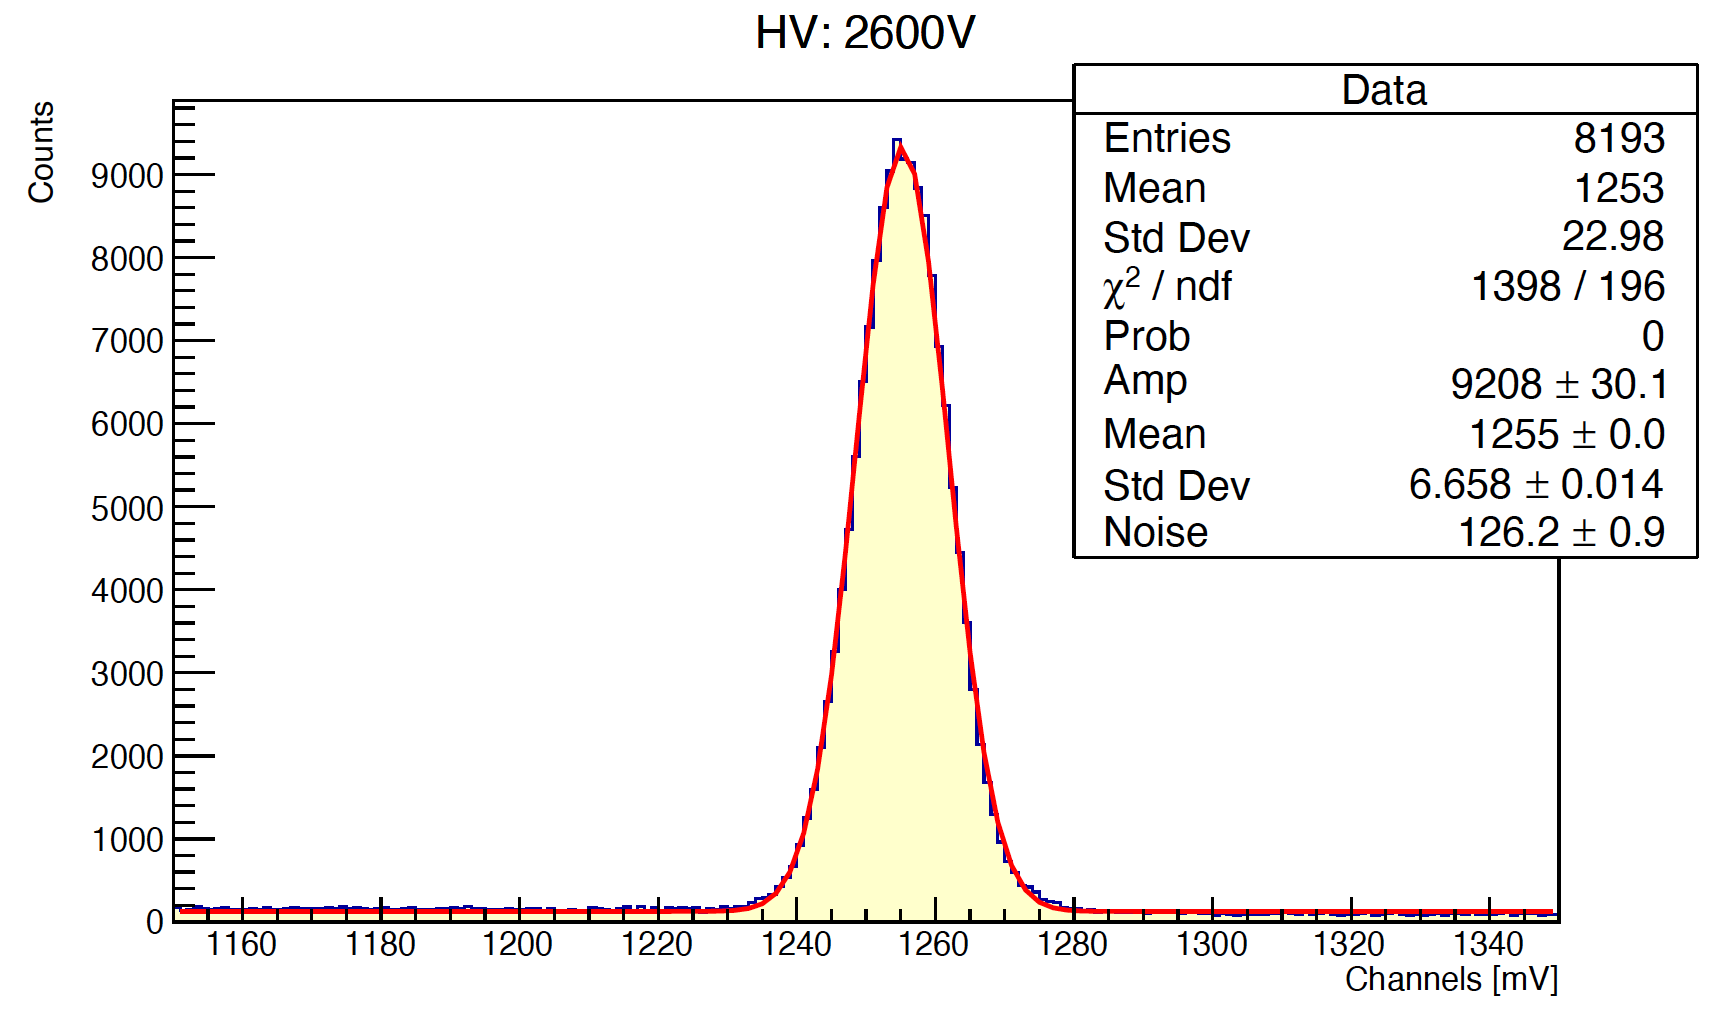
\includegraphics[scale=0.45]{appendice/2600}
\end{figure}
\begin{figure}[H]
    \centering
    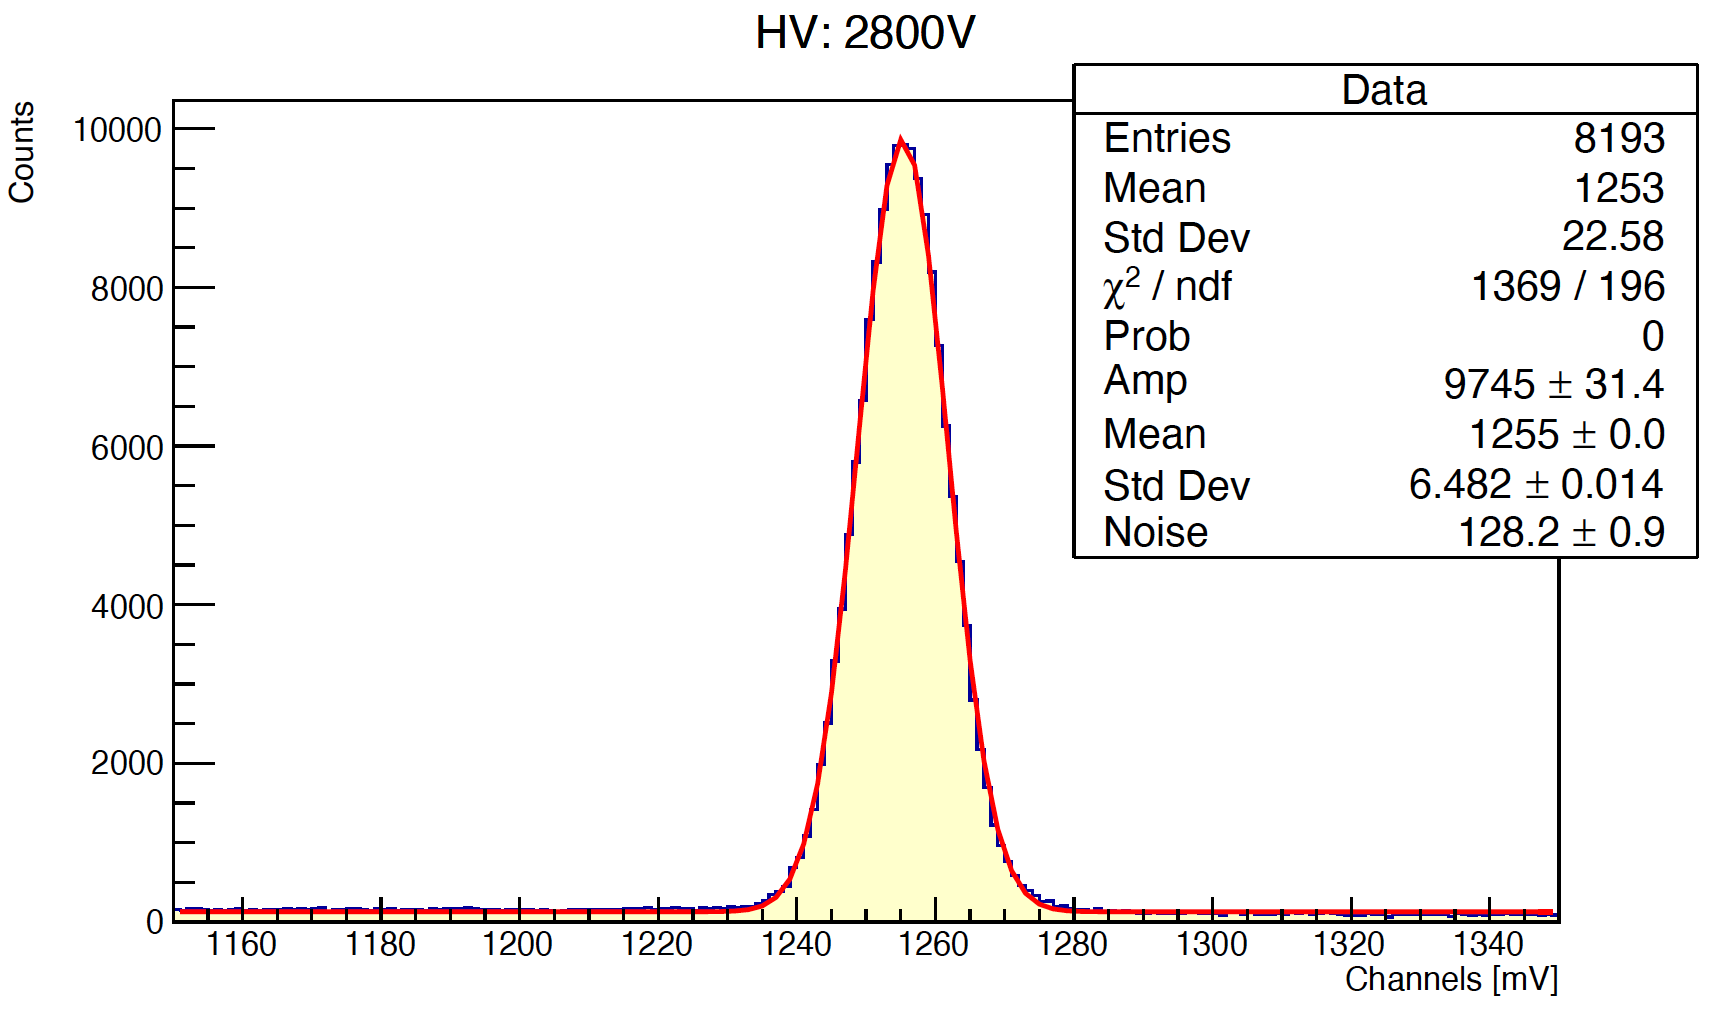
\includegraphics[scale=0.45]{appendice/2800}
\end{figure}
\begin{figure}[H]
    \centering
    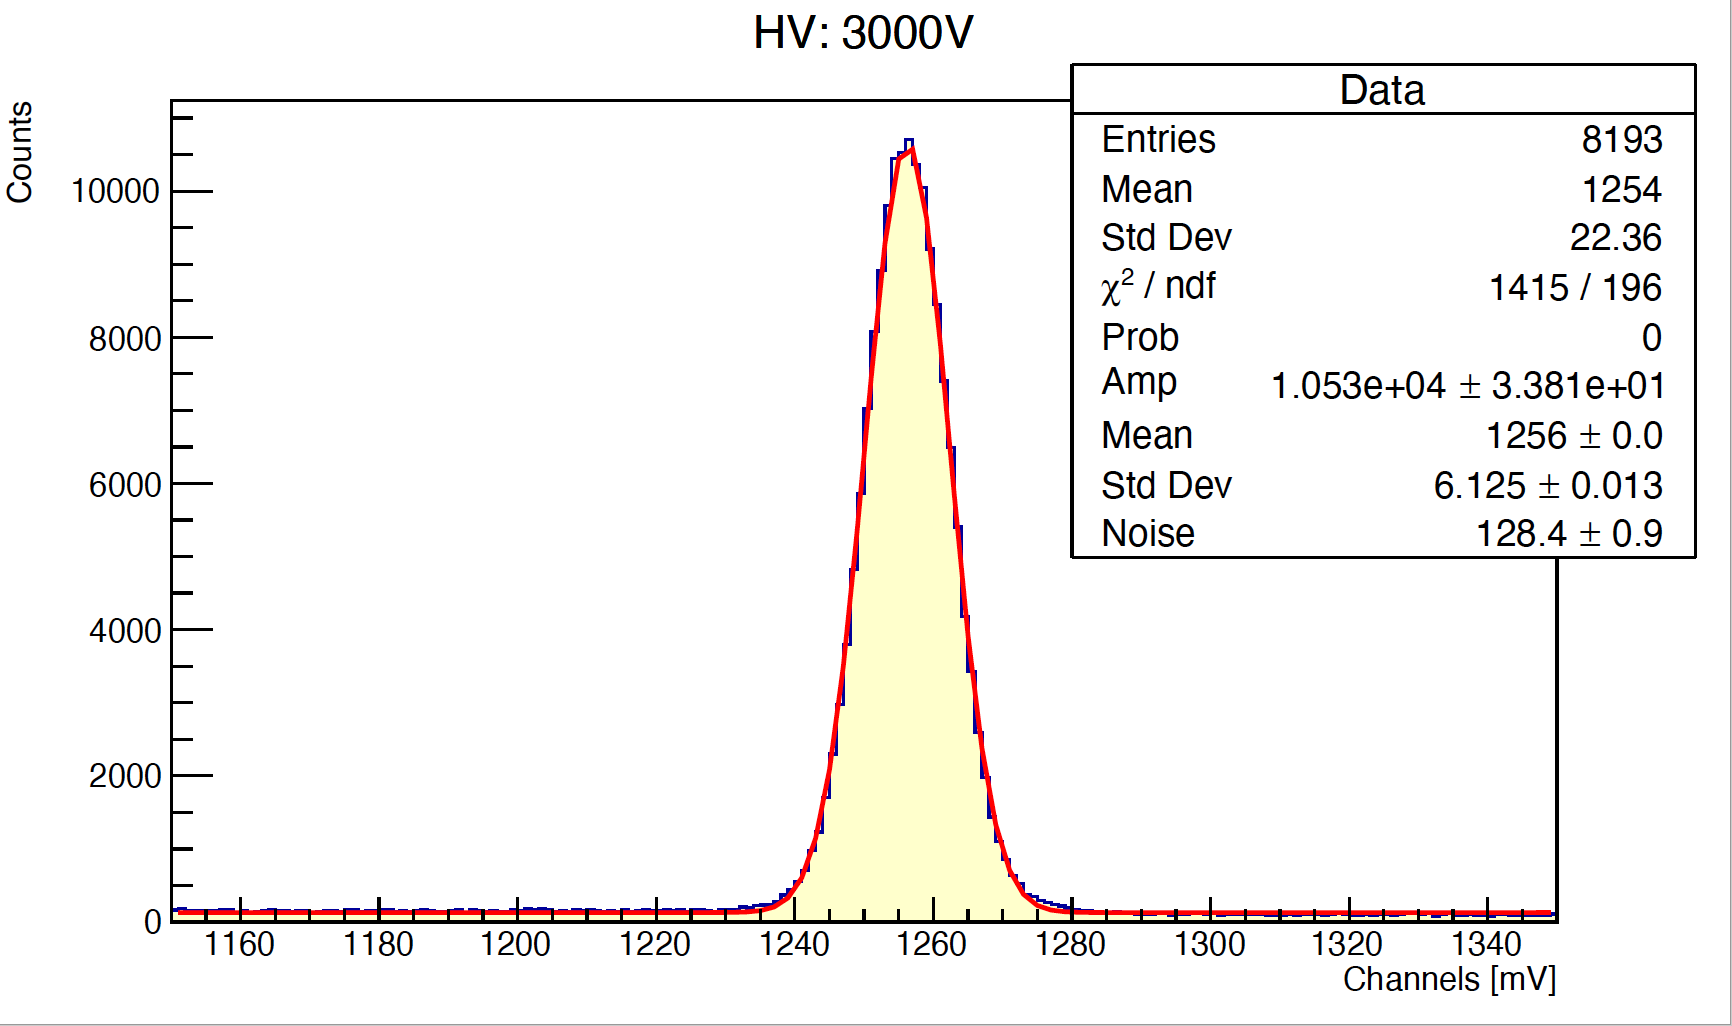
\includegraphics[scale=0.45]{appendice/3000}
\end{figure}
\begin{figure}[H]
    \centering
    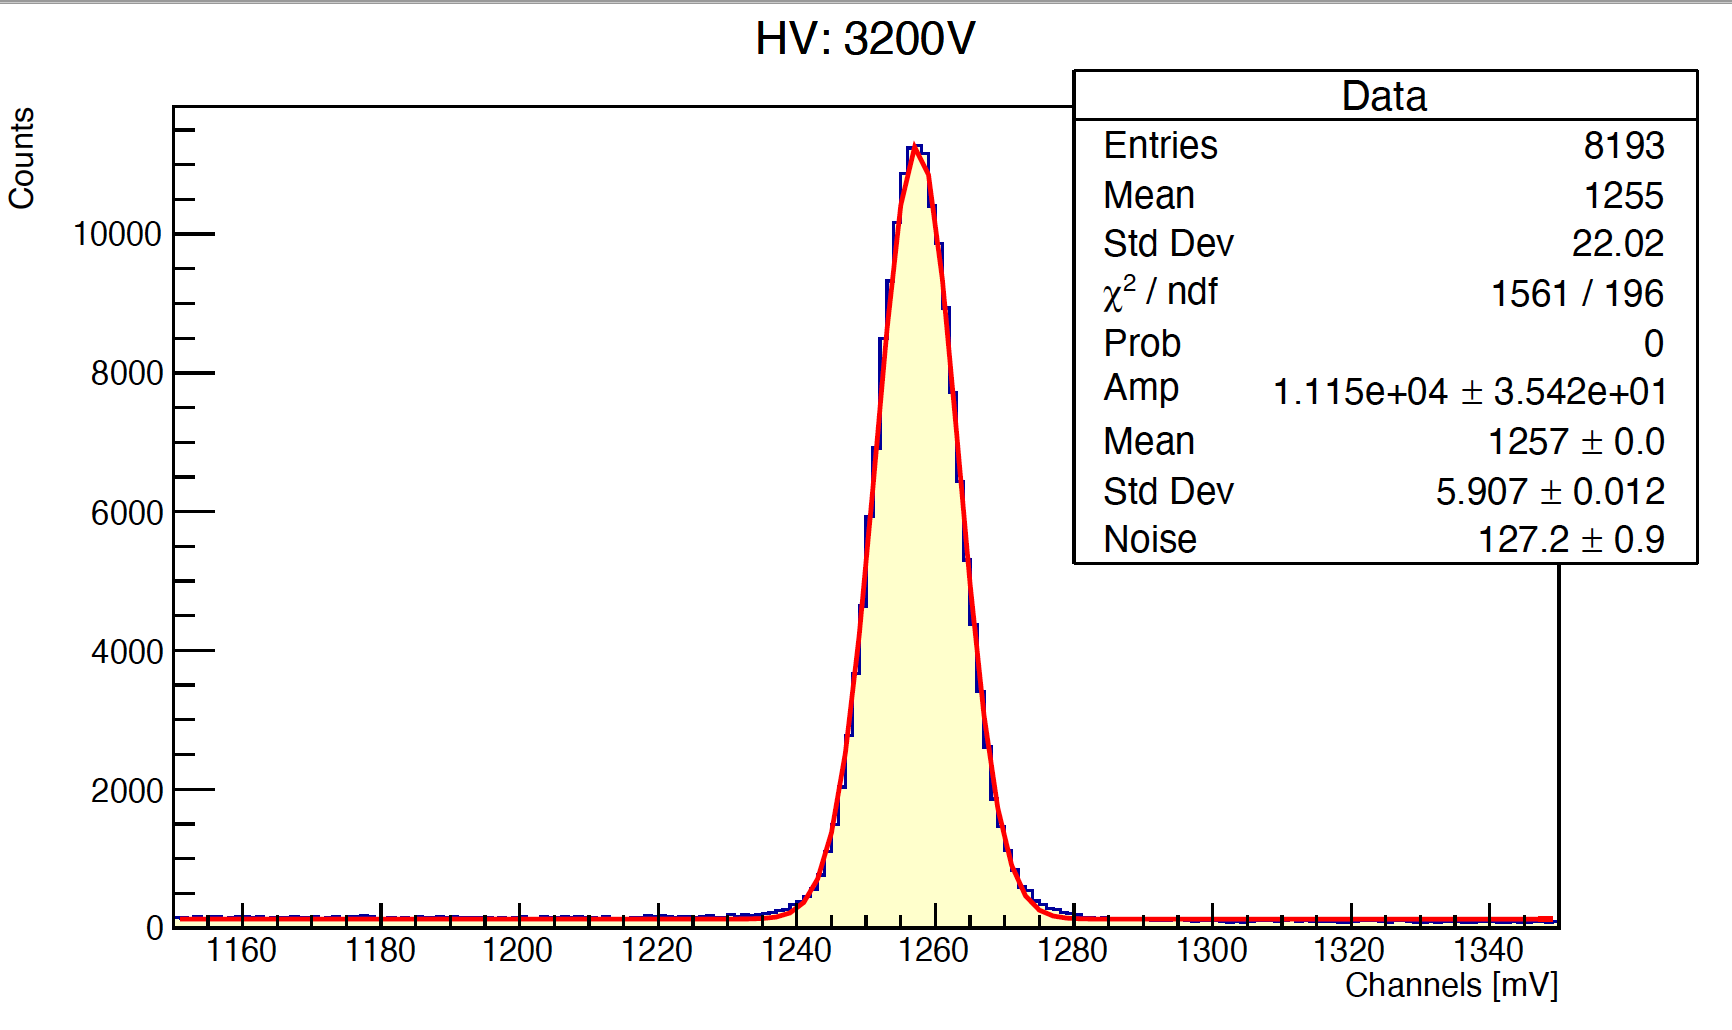
\includegraphics[scale=0.45]{appendice/3200}
\end{figure}
\begin{figure}[H]
    \centering
    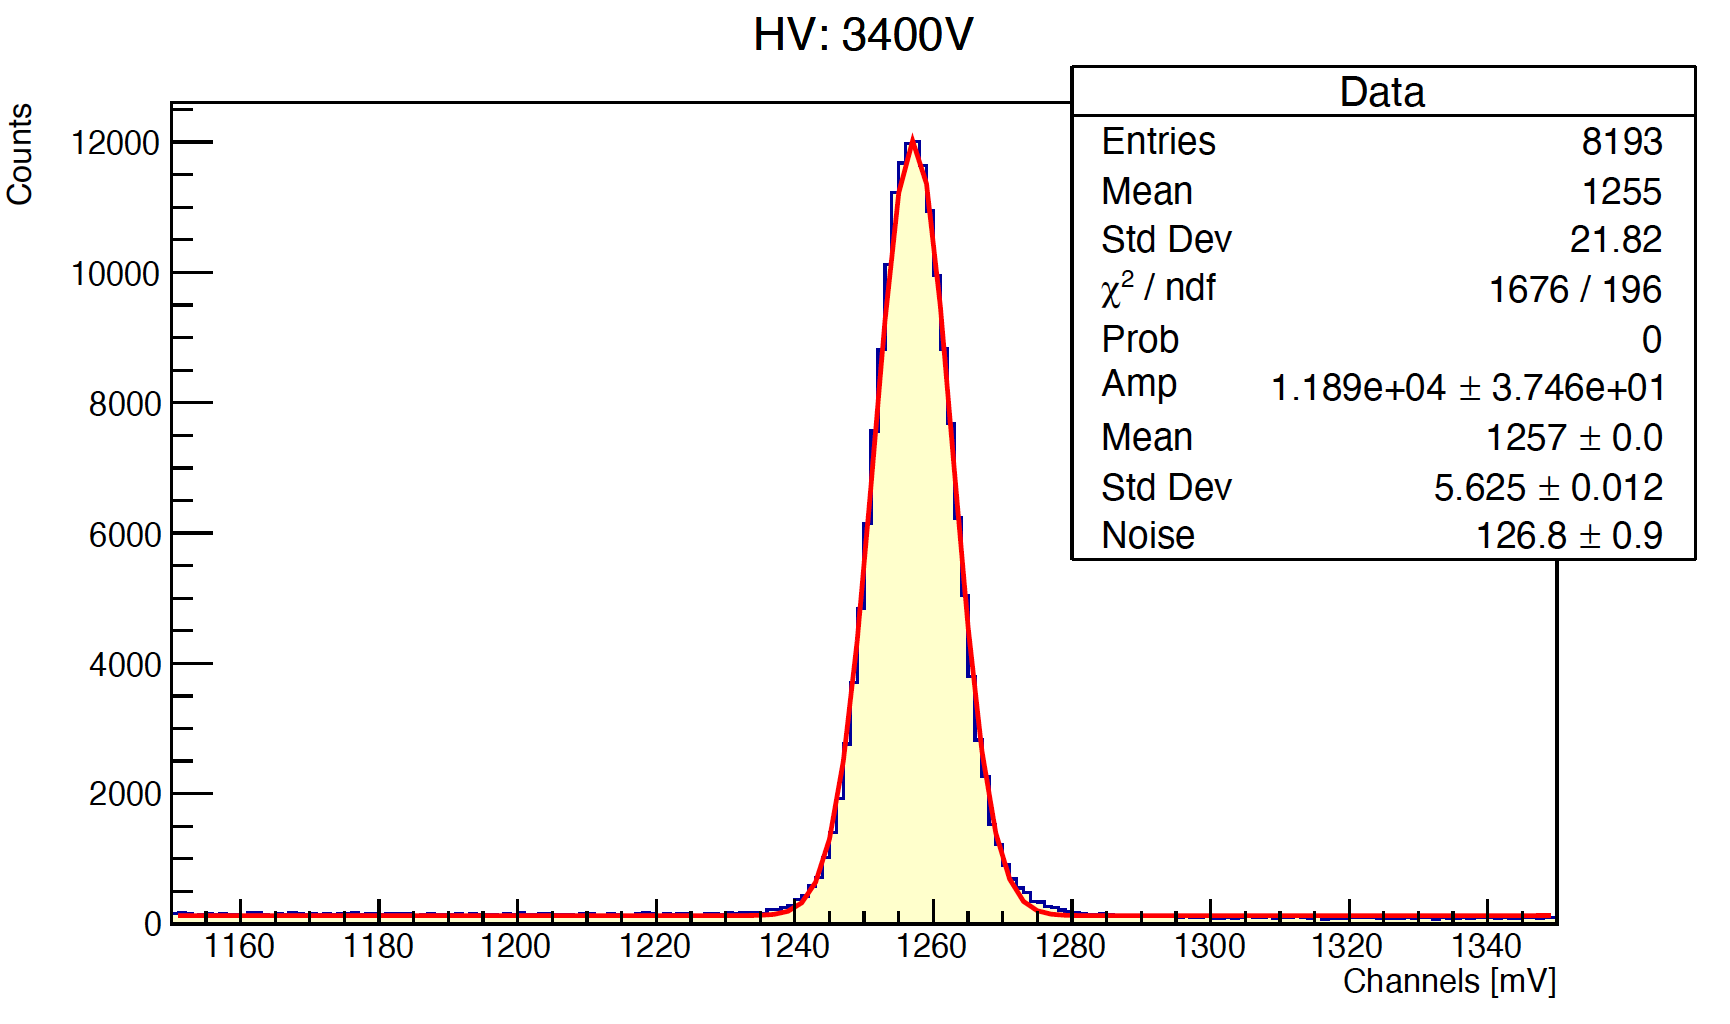
\includegraphics[scale=0.45]{appendice/3400}
\end{figure}
\begin{figure}[H]
    \centering
    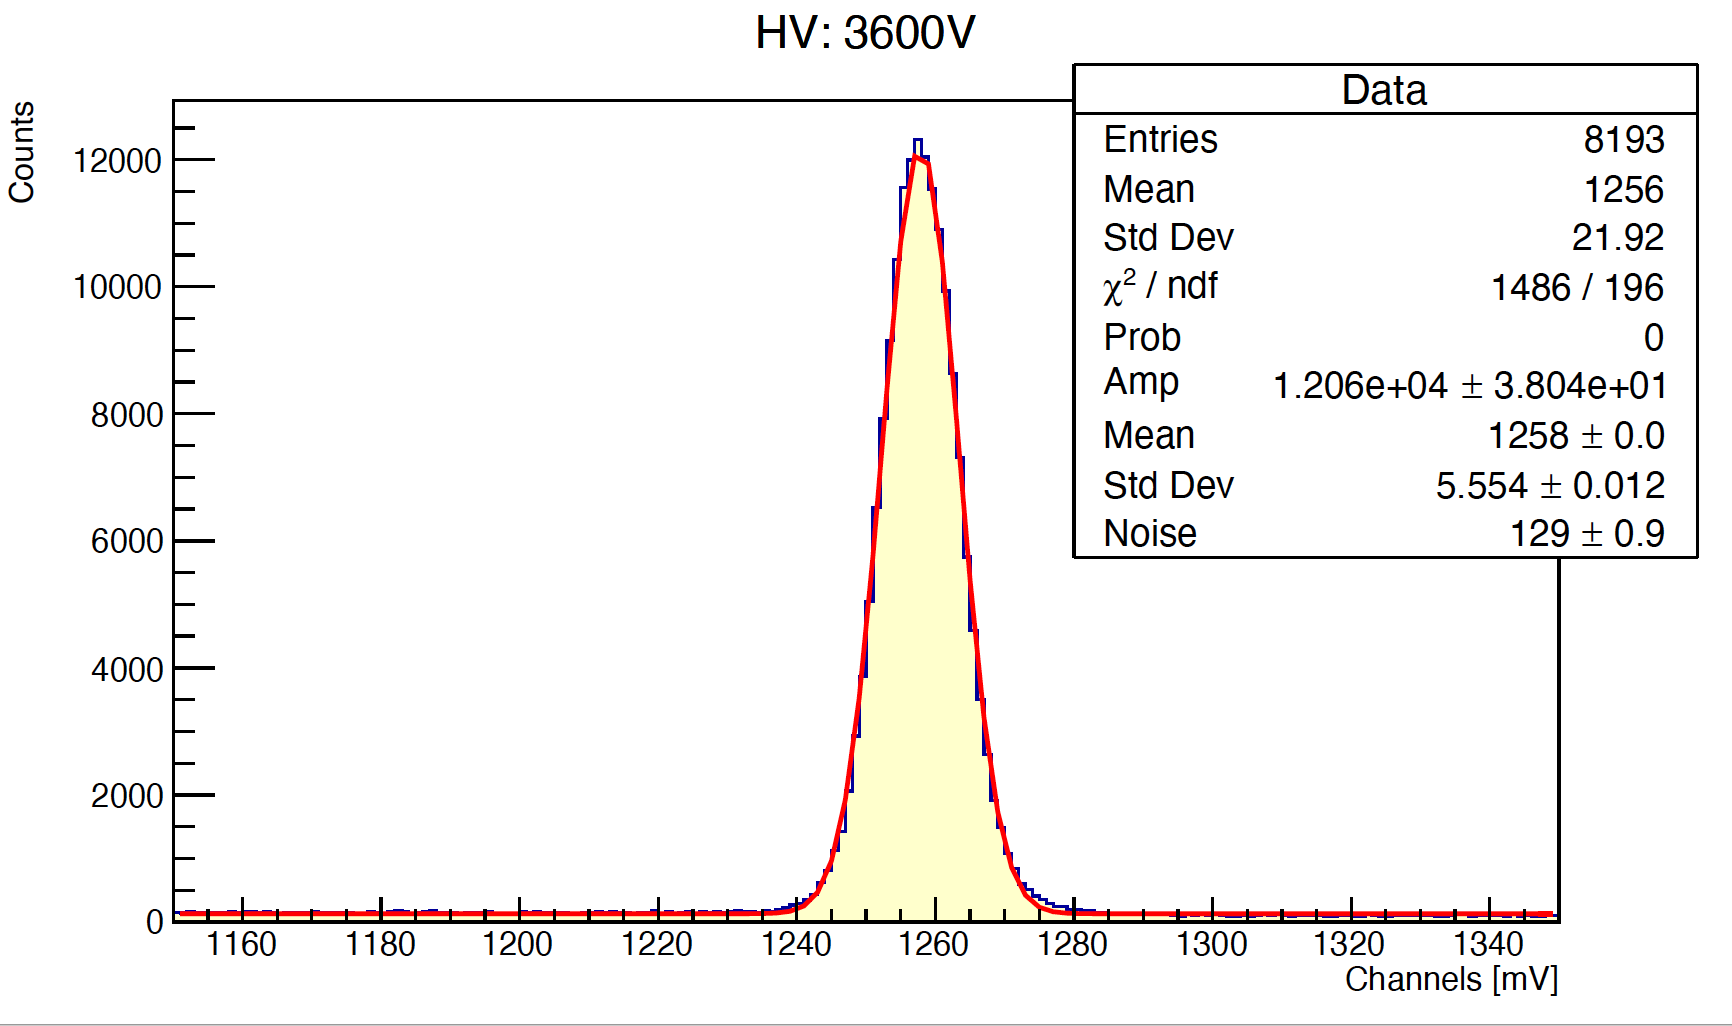
\includegraphics[scale=0.45]{appendice/3600}
\end{figure}
\begin{figure}[H]
    \centering
    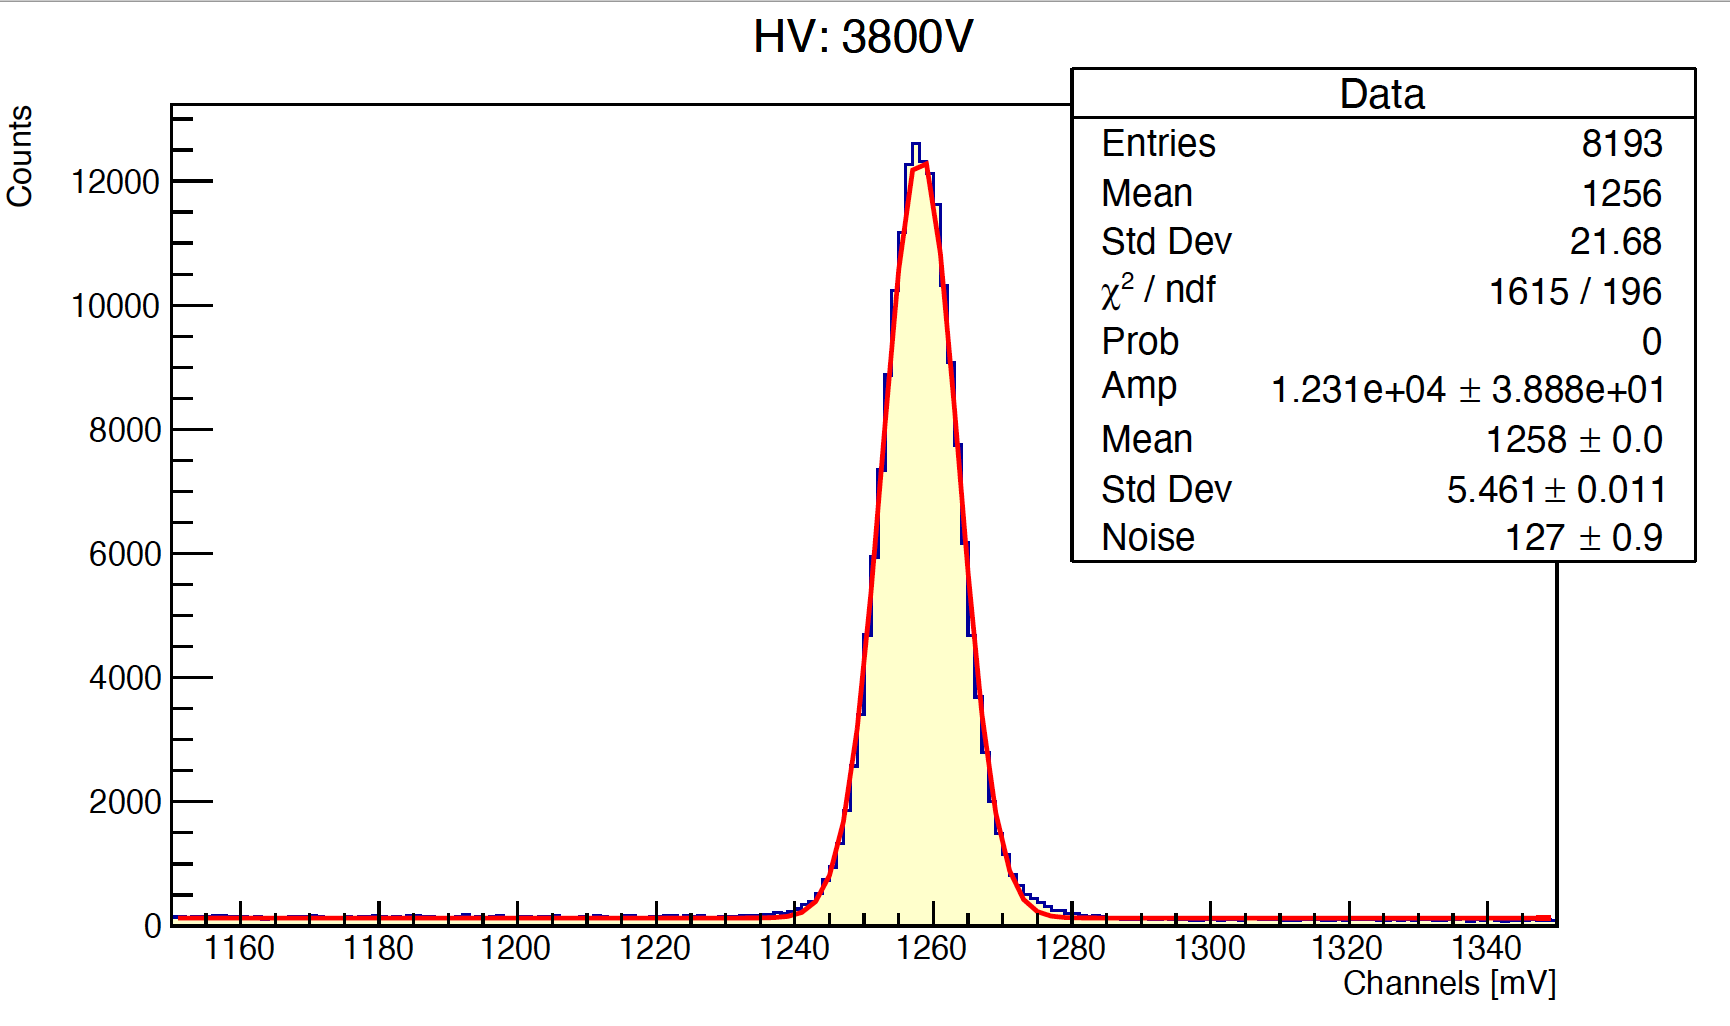
\includegraphics[scale=0.45]{appendice/3800}
\end{figure}
\begin{figure}[H]
    \centering
    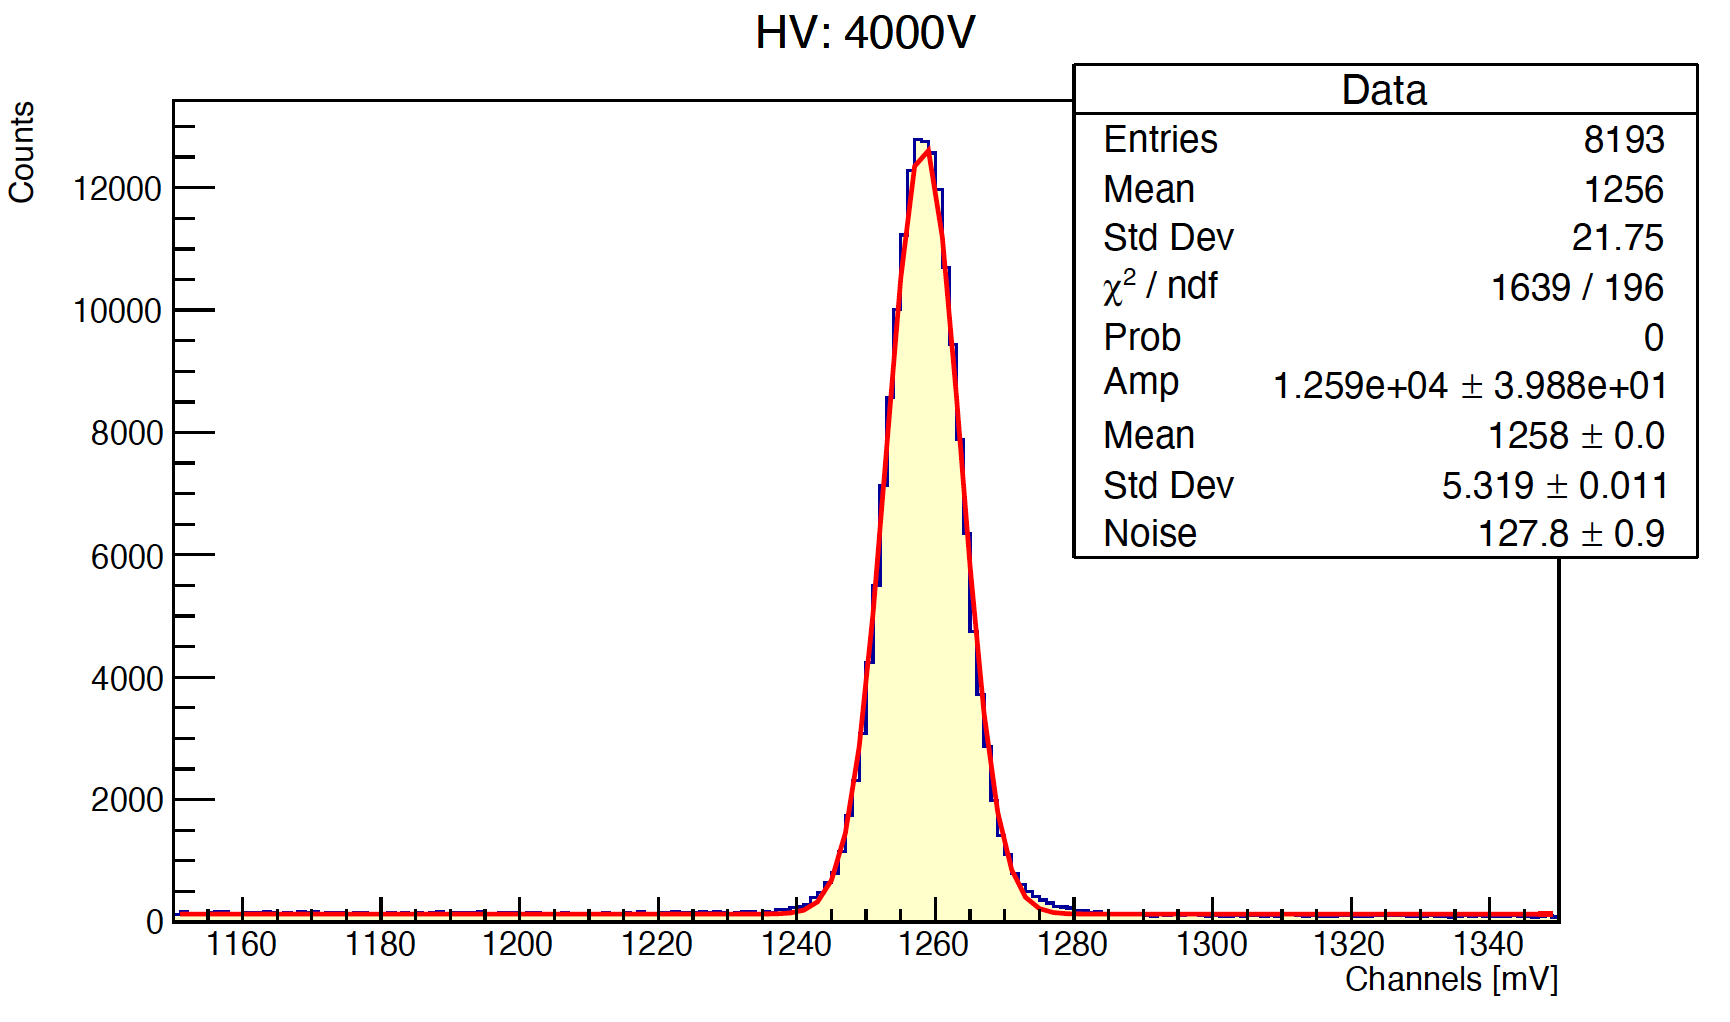
\includegraphics[scale=0.45]{appendice/4000}
\end{figure}
\begin{figure}[H]
    \centering
    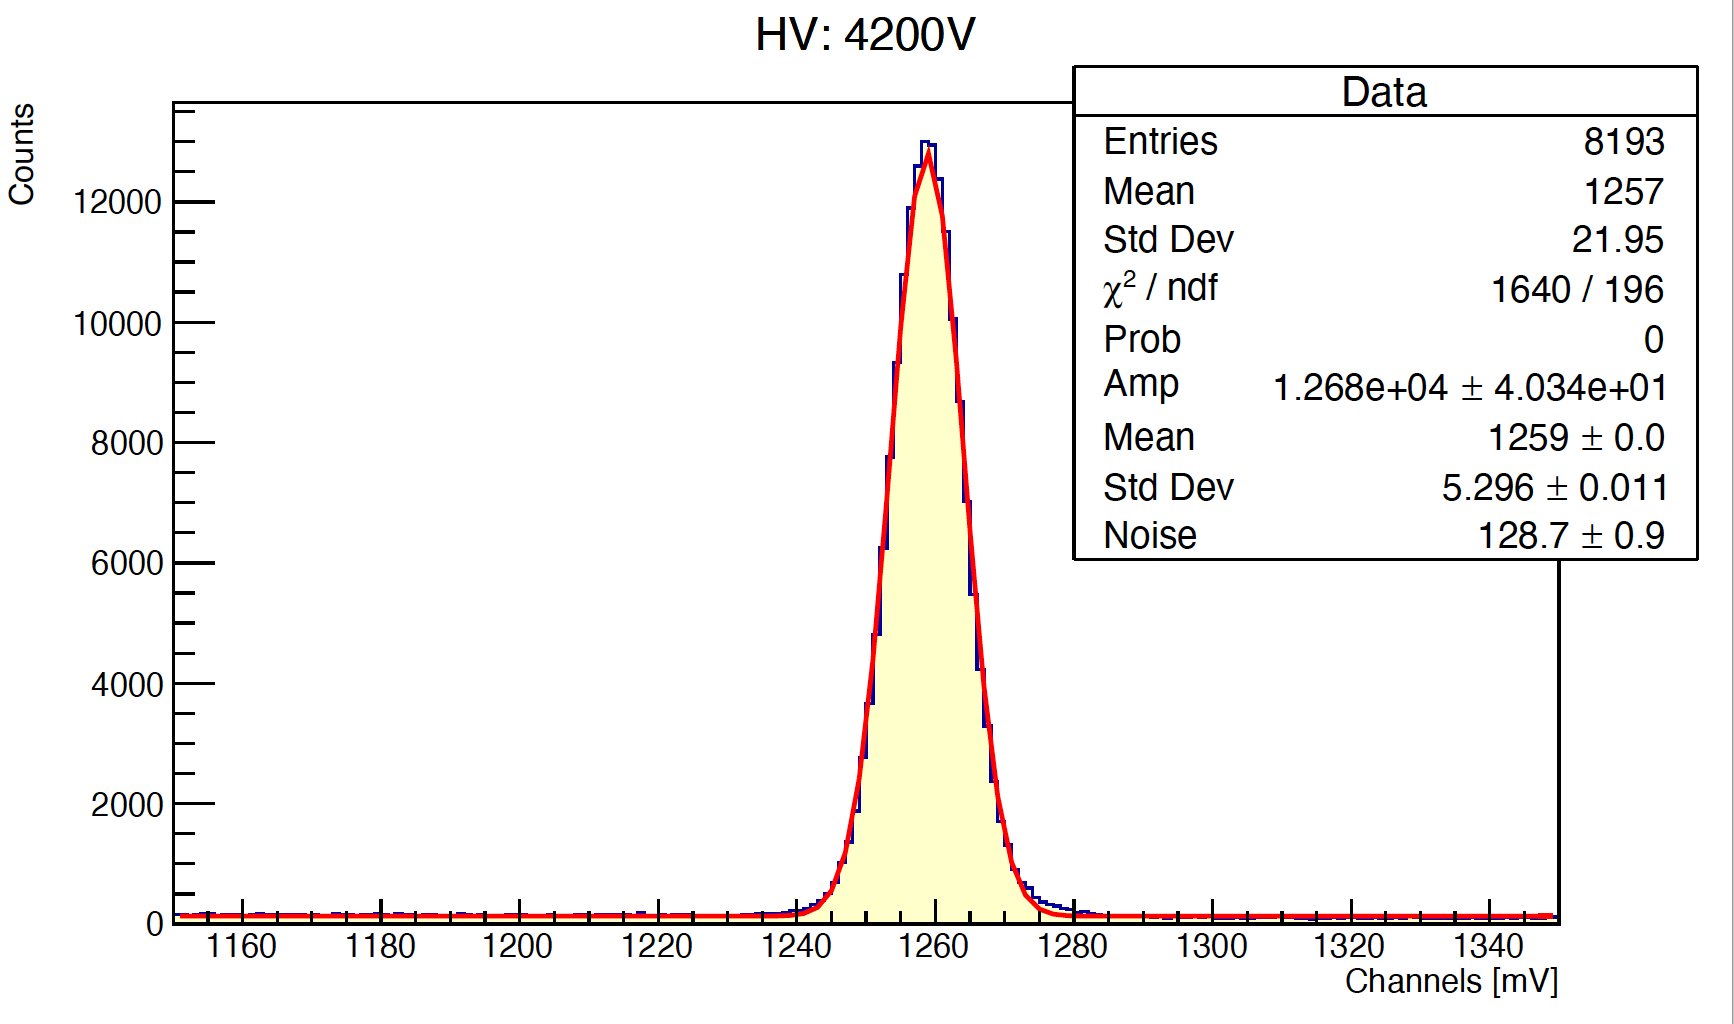
\includegraphics[scale=0.45]{appendice/4200}
\end{figure}
\begin{figure}[H]
    \centering
    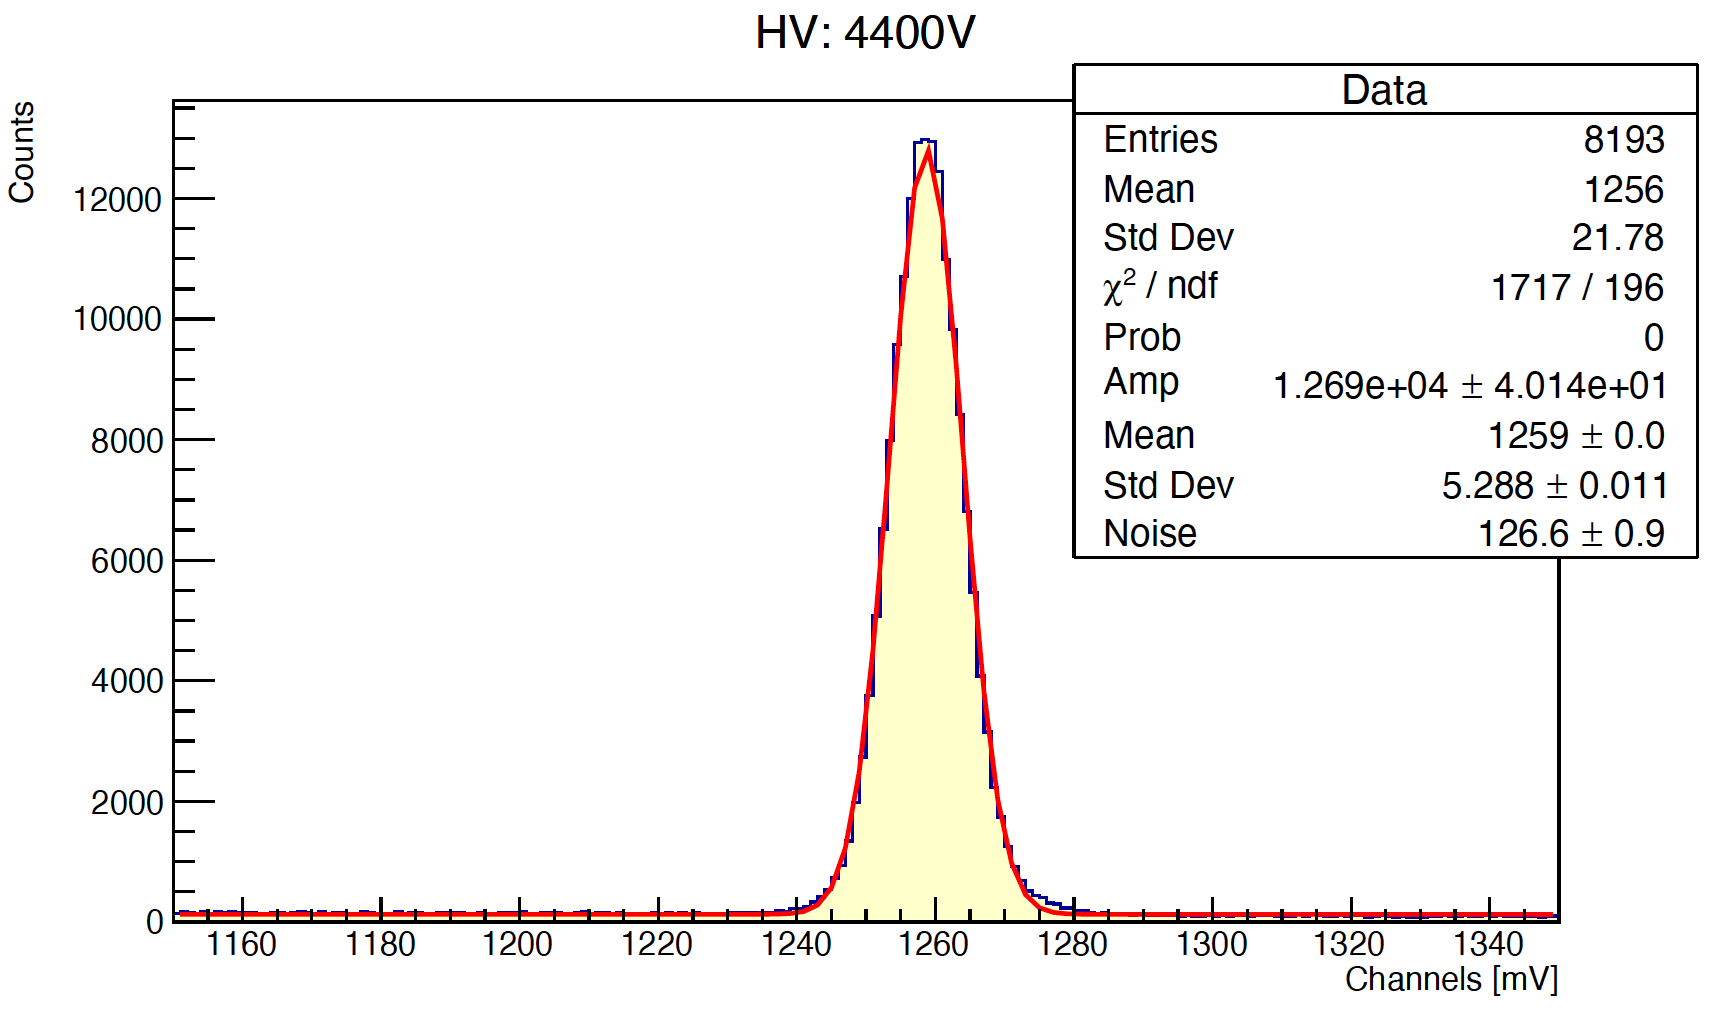
\includegraphics[scale=0.45]{appendice/4400}
\end{figure}
\begin{figure}[H]
    \centering
    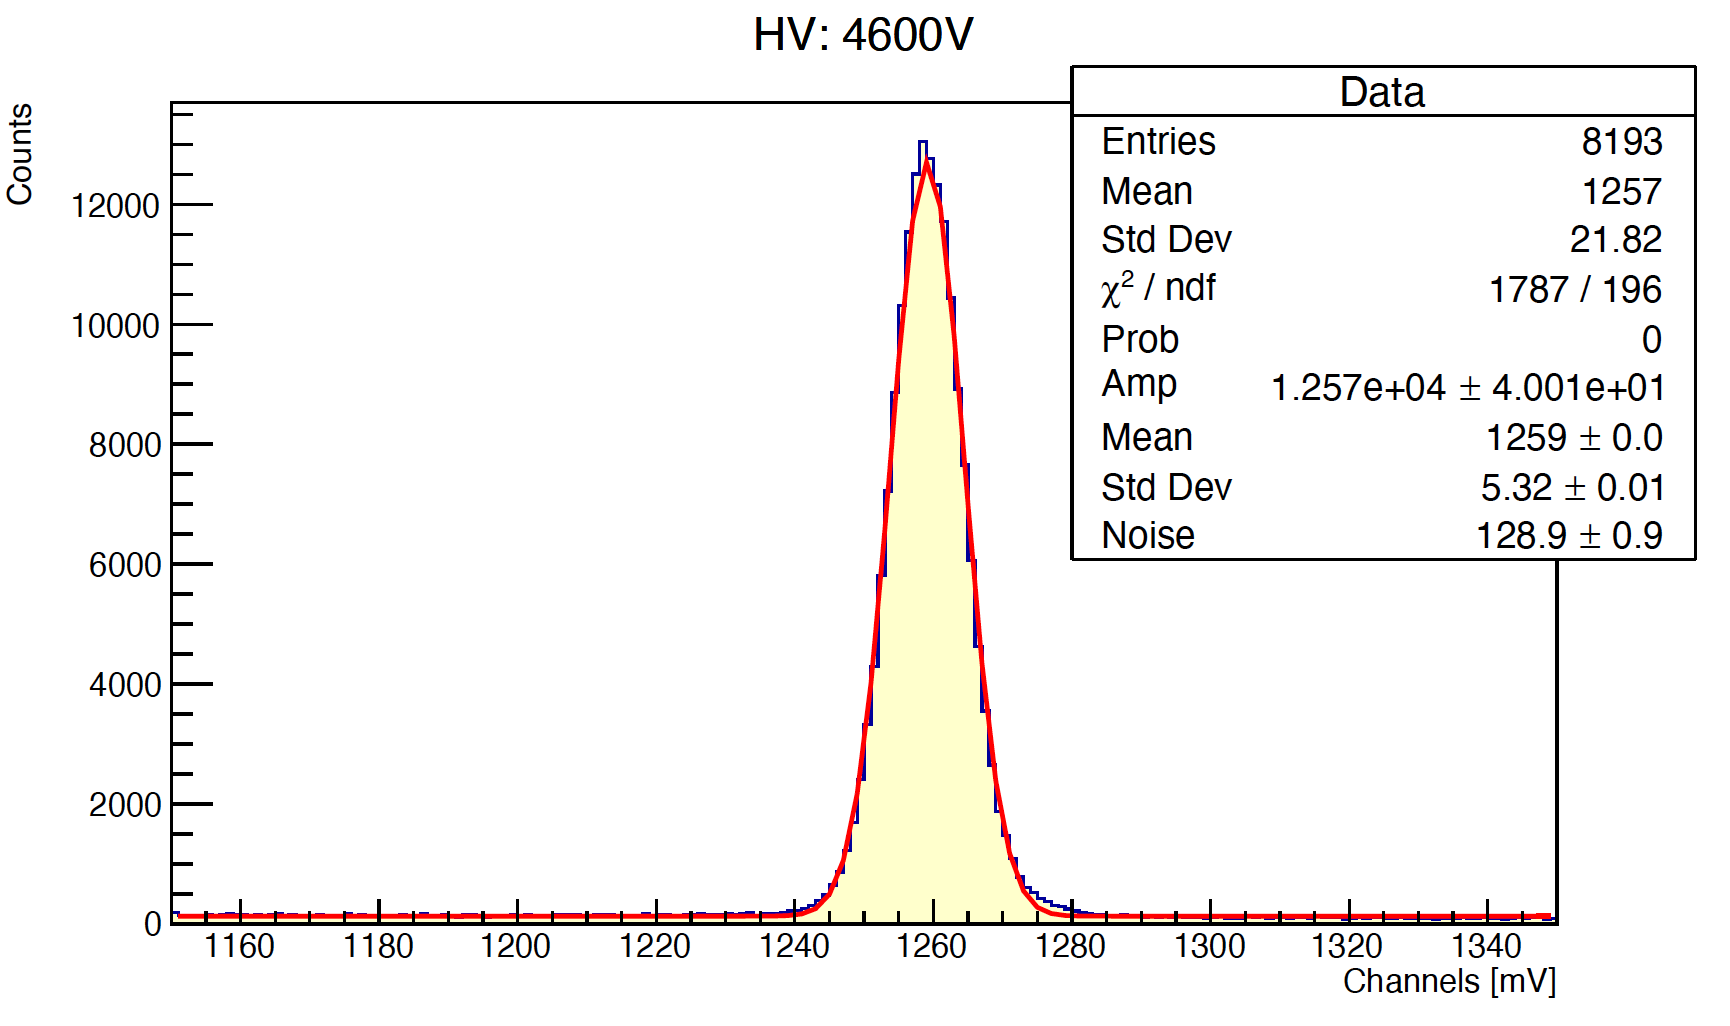
\includegraphics[scale=0.45]{appendice/4600}
\end{figure}
\begin{figure}[H]
    \centering
    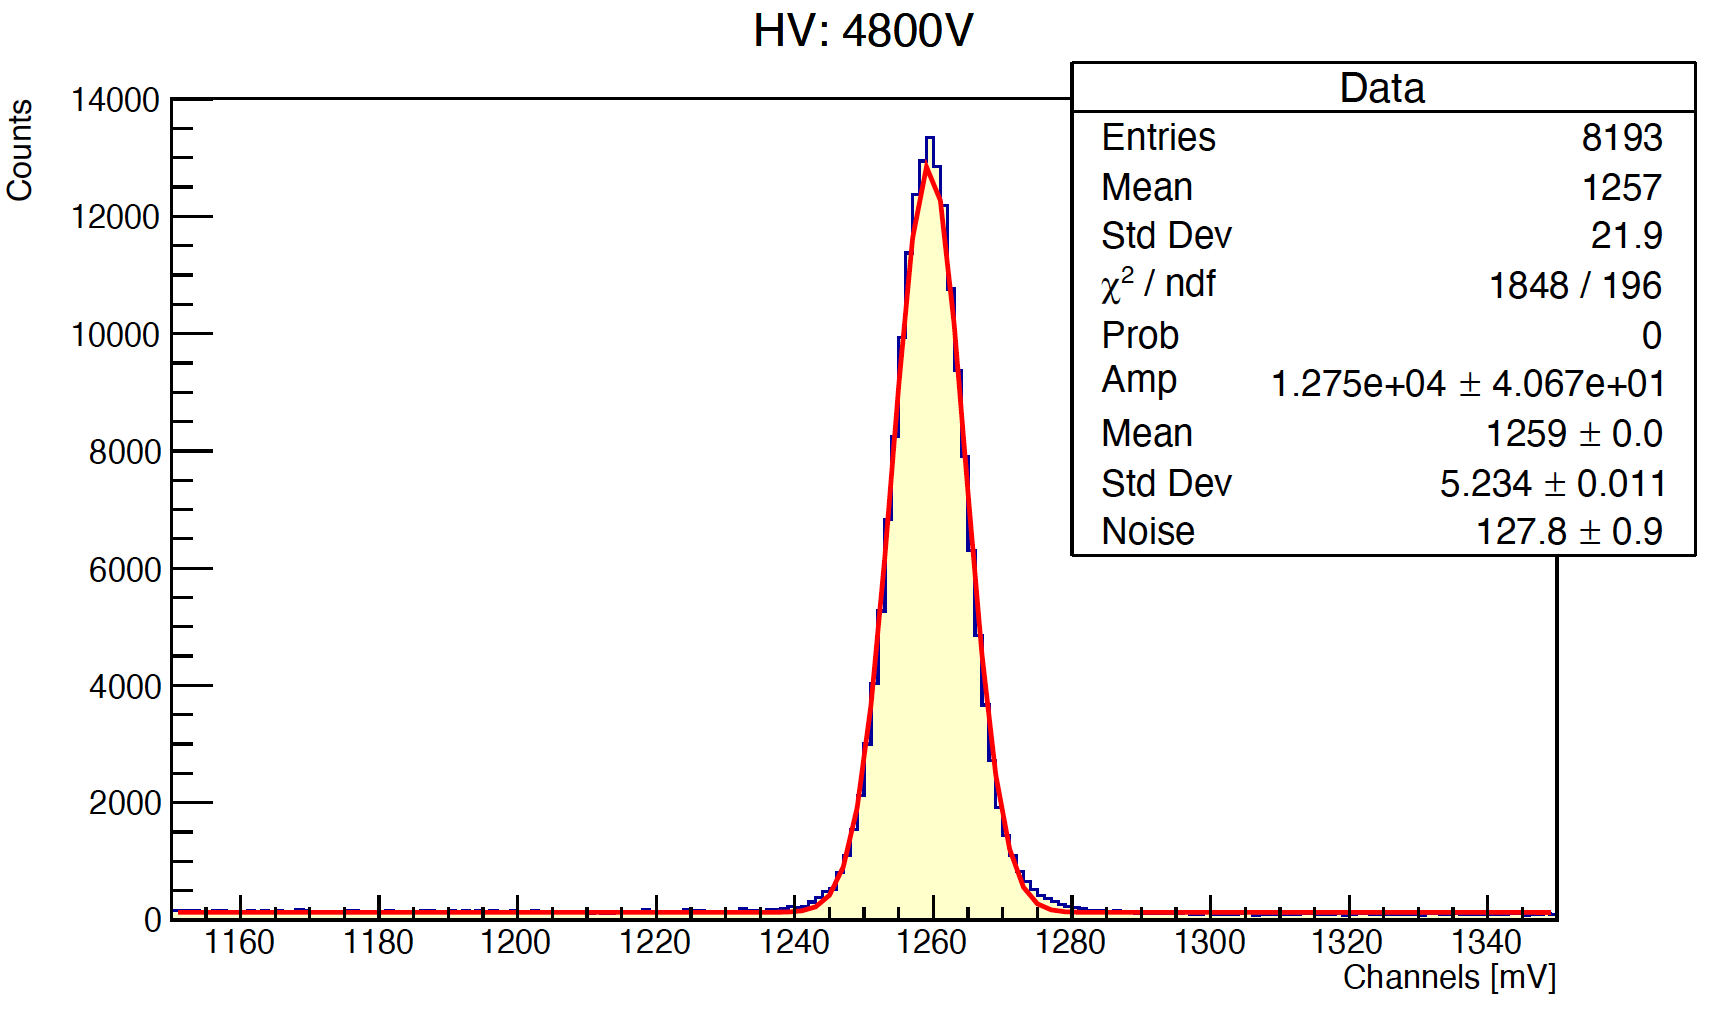
\includegraphics[scale=0.45]{appendice/4800}
\end{figure}
\begin{figure}[H]
    \centering
    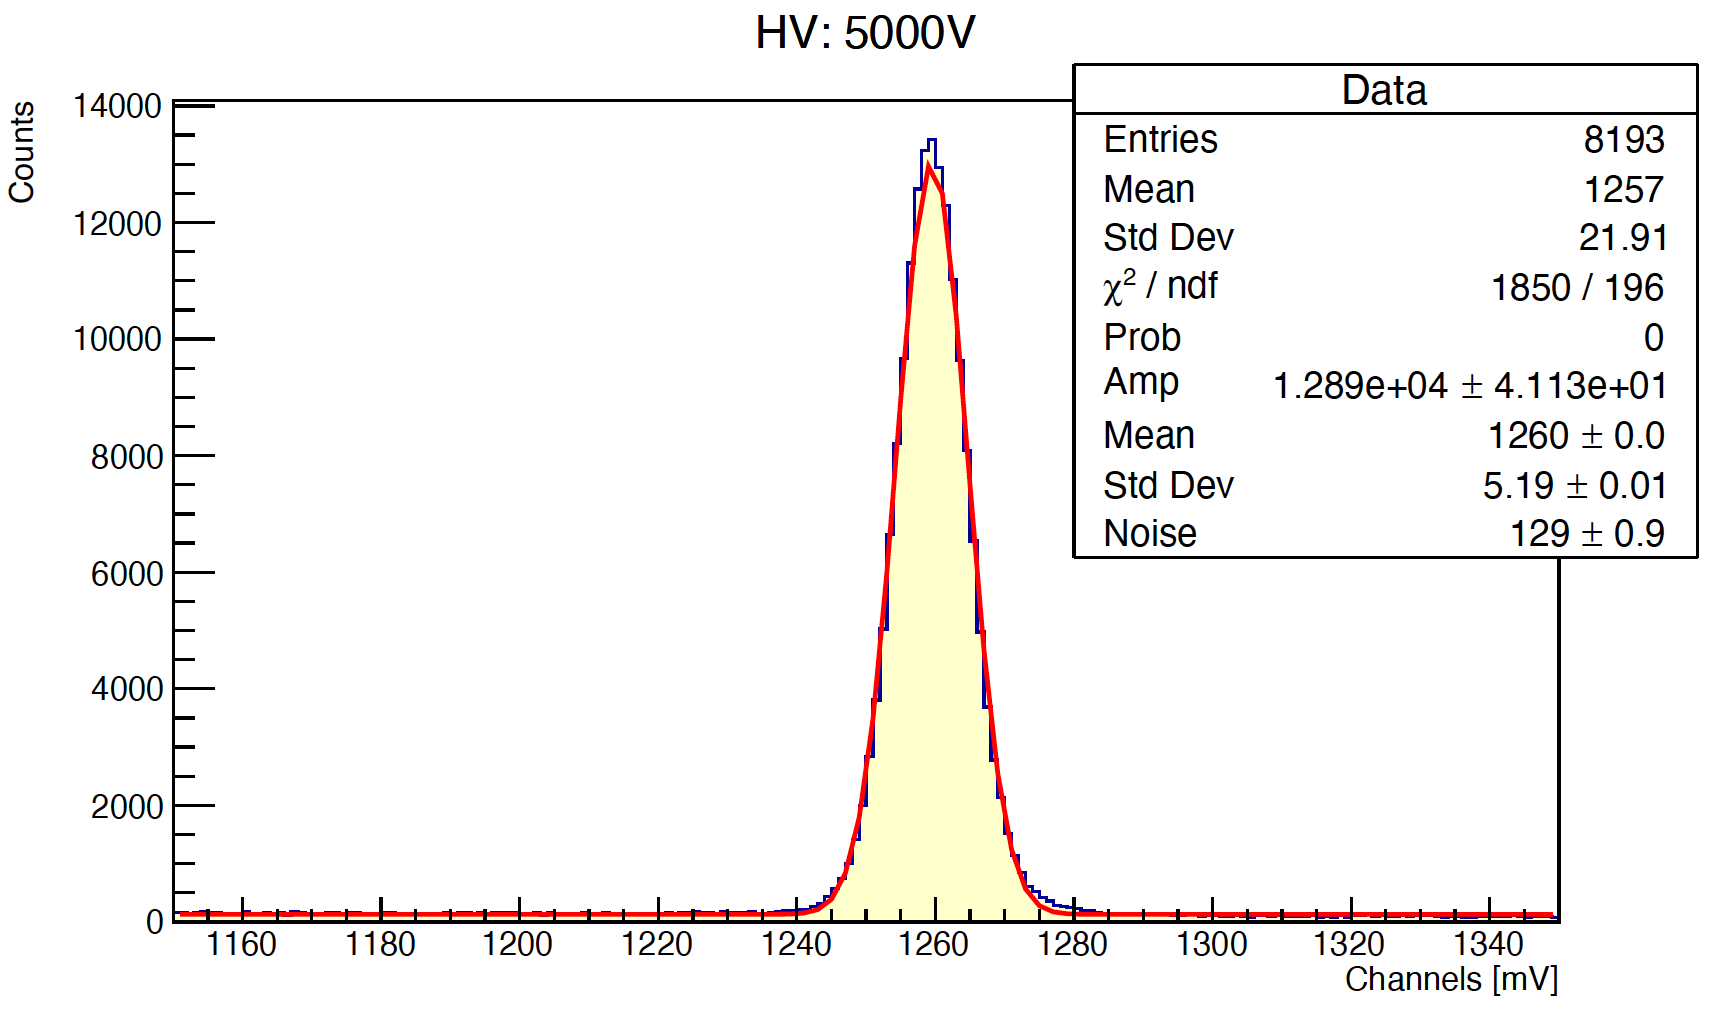
\includegraphics[scale=0.45]{appendice/5000}
\end{figure}

%%% SHAPING TIME %%%
\subsection{Shaping Time}
\begin{figure}[H]
    \centering
    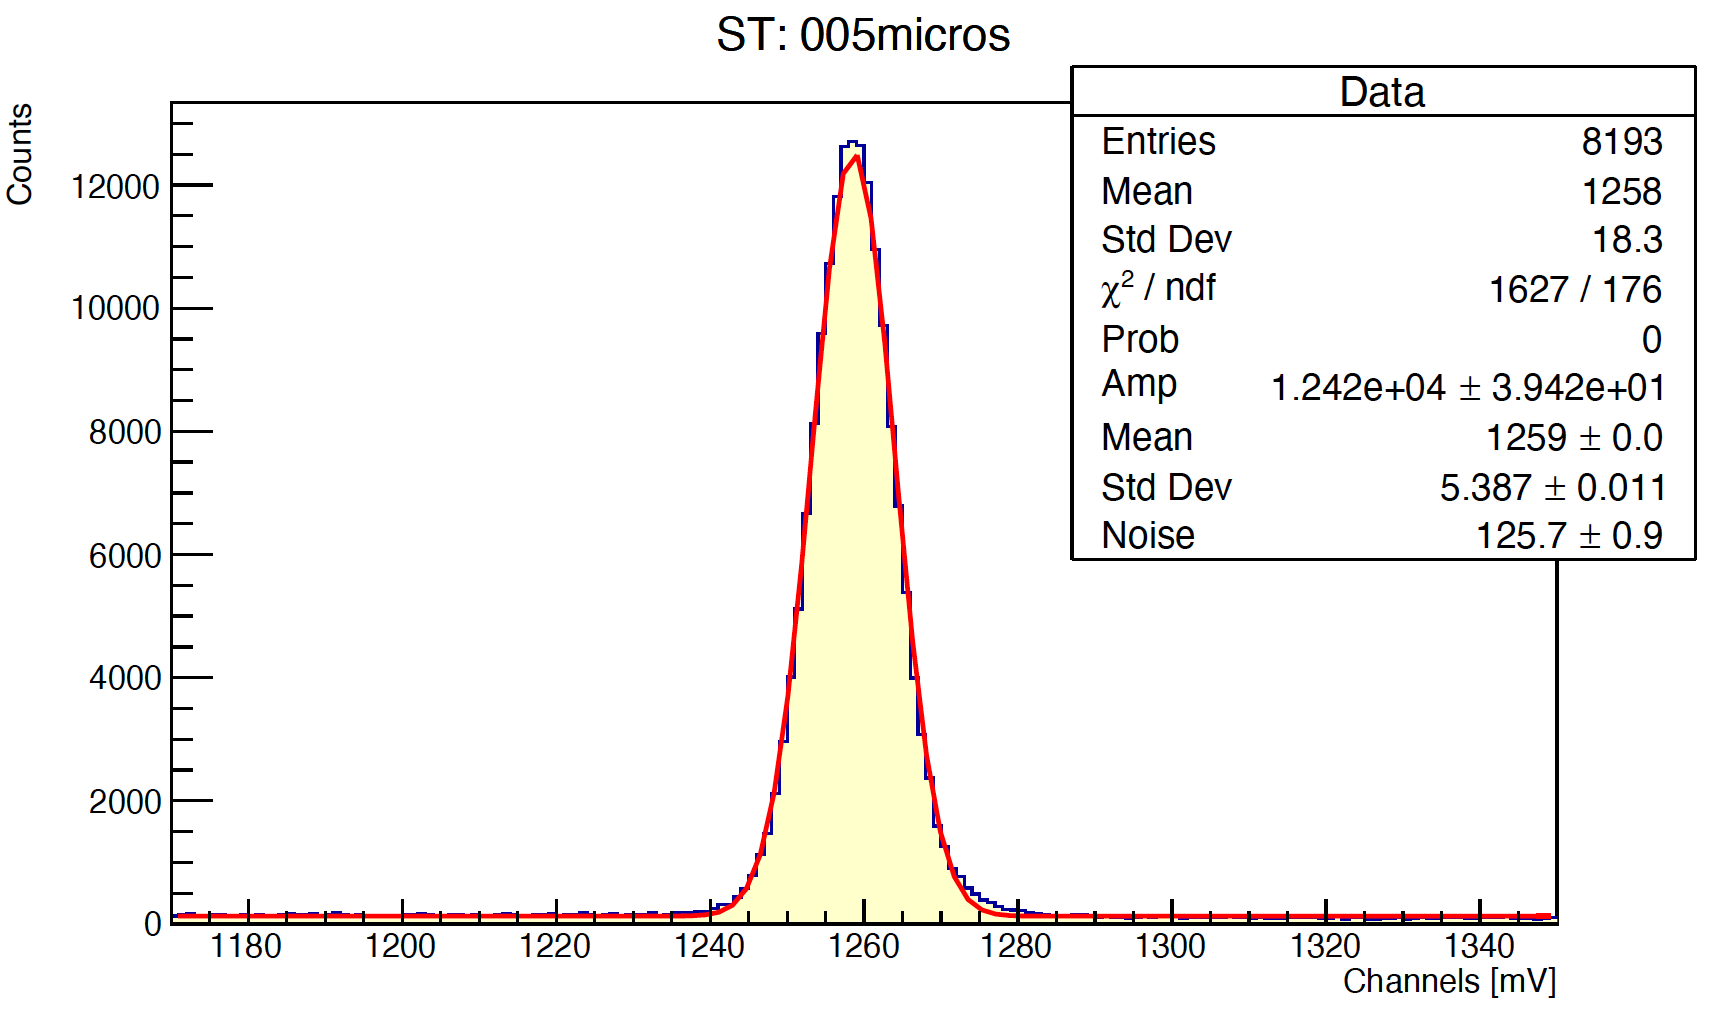
\includegraphics[scale=0.45]{appendice/5}
\end{figure}
\begin{figure}[H]
    \centering
    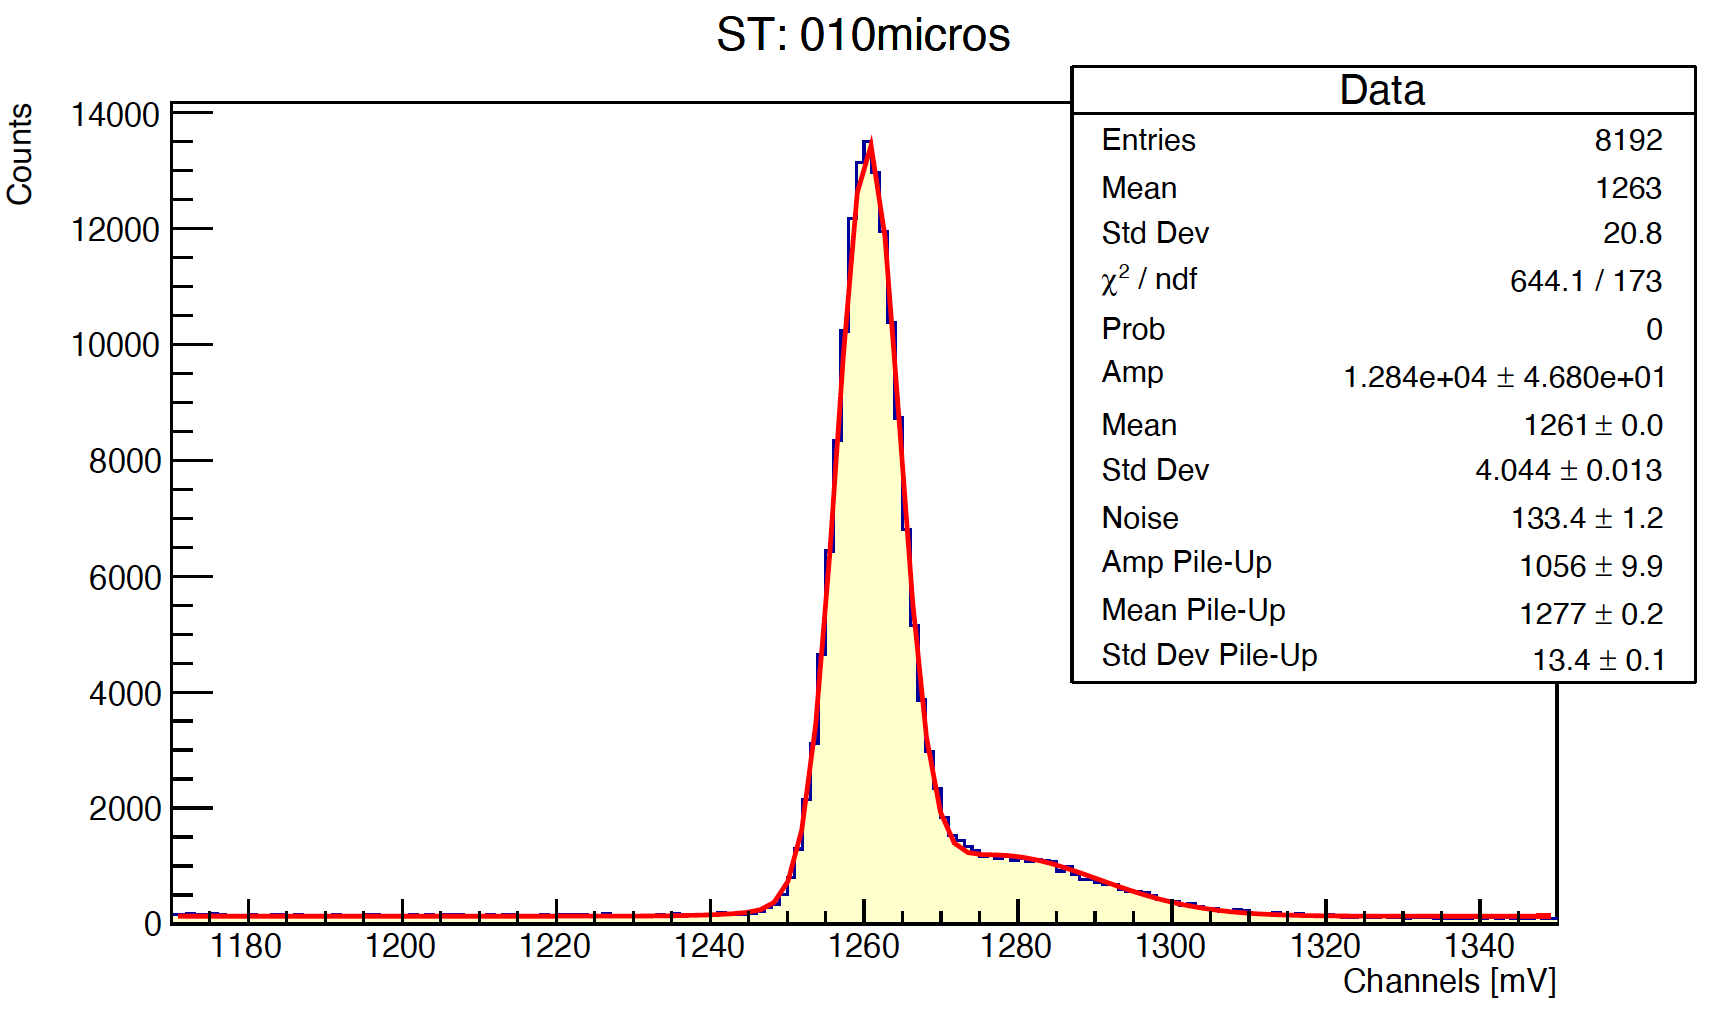
\includegraphics[scale=0.45]{appendice/10}
\end{figure}
\begin{figure}[H]
    \centering
    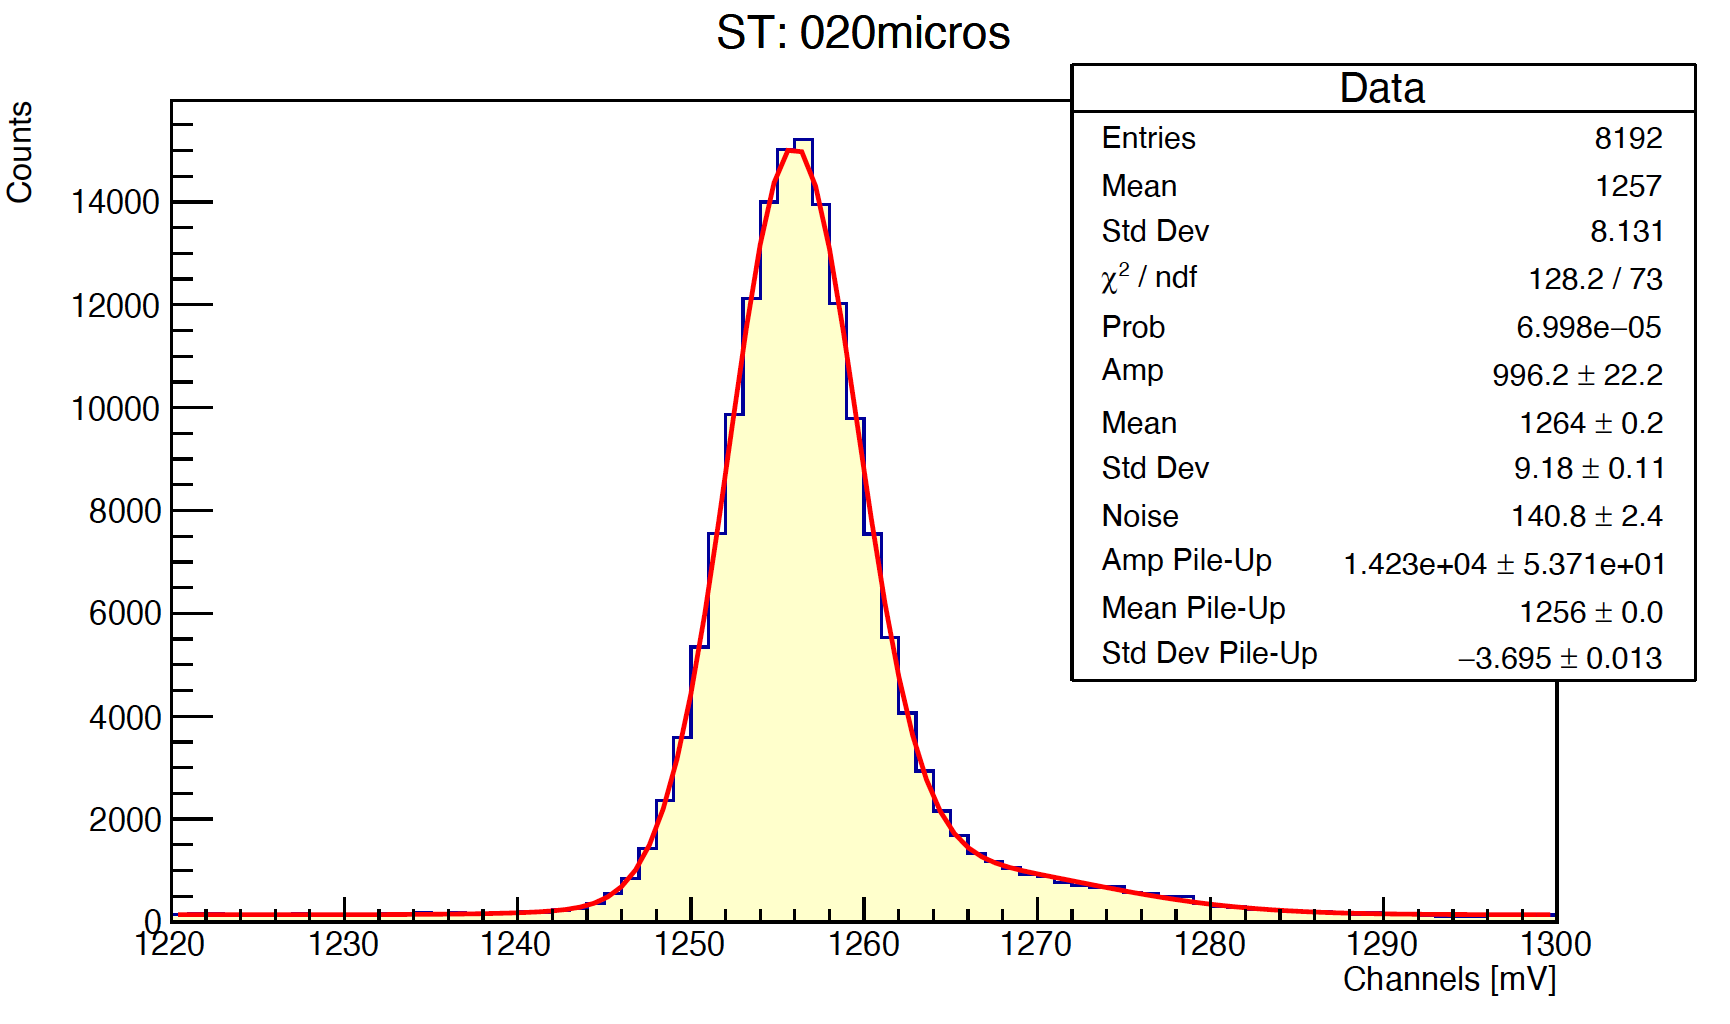
\includegraphics[scale=0.45]{appendice/20}
\end{figure}
\begin{figure}[H]
    \centering
    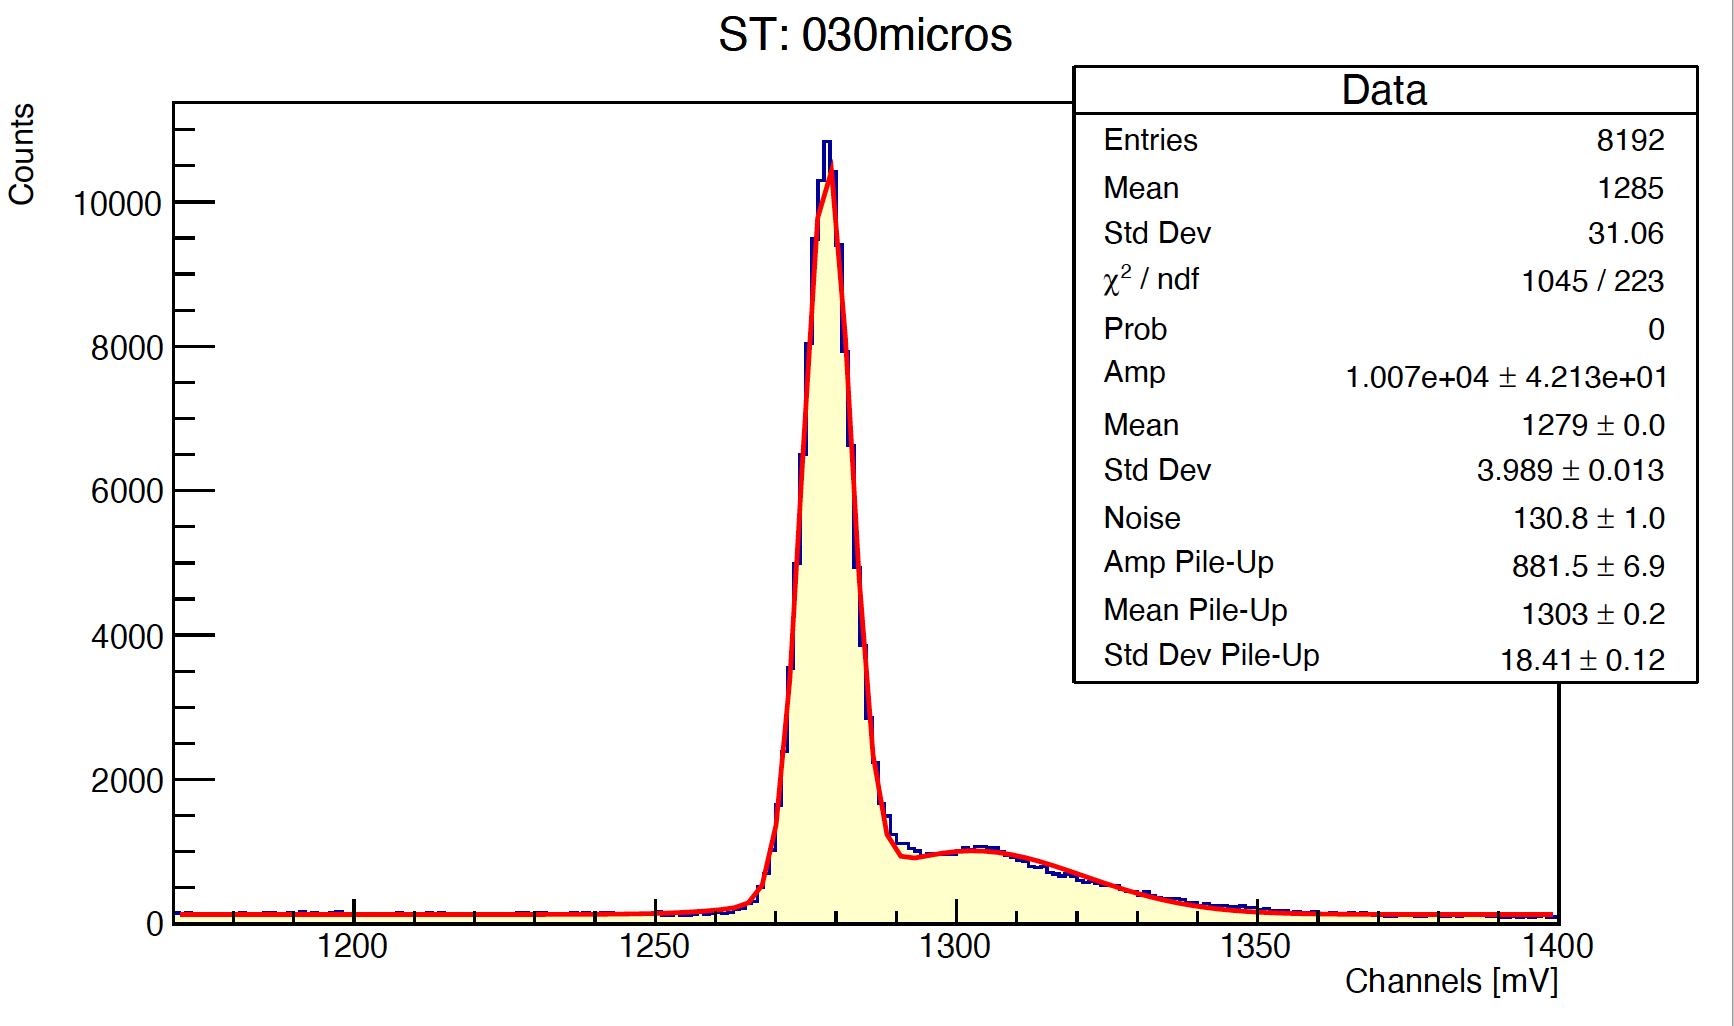
\includegraphics[scale=0.45]{appendice/30}
\end{figure}
\begin{figure}[H]
    \centering
    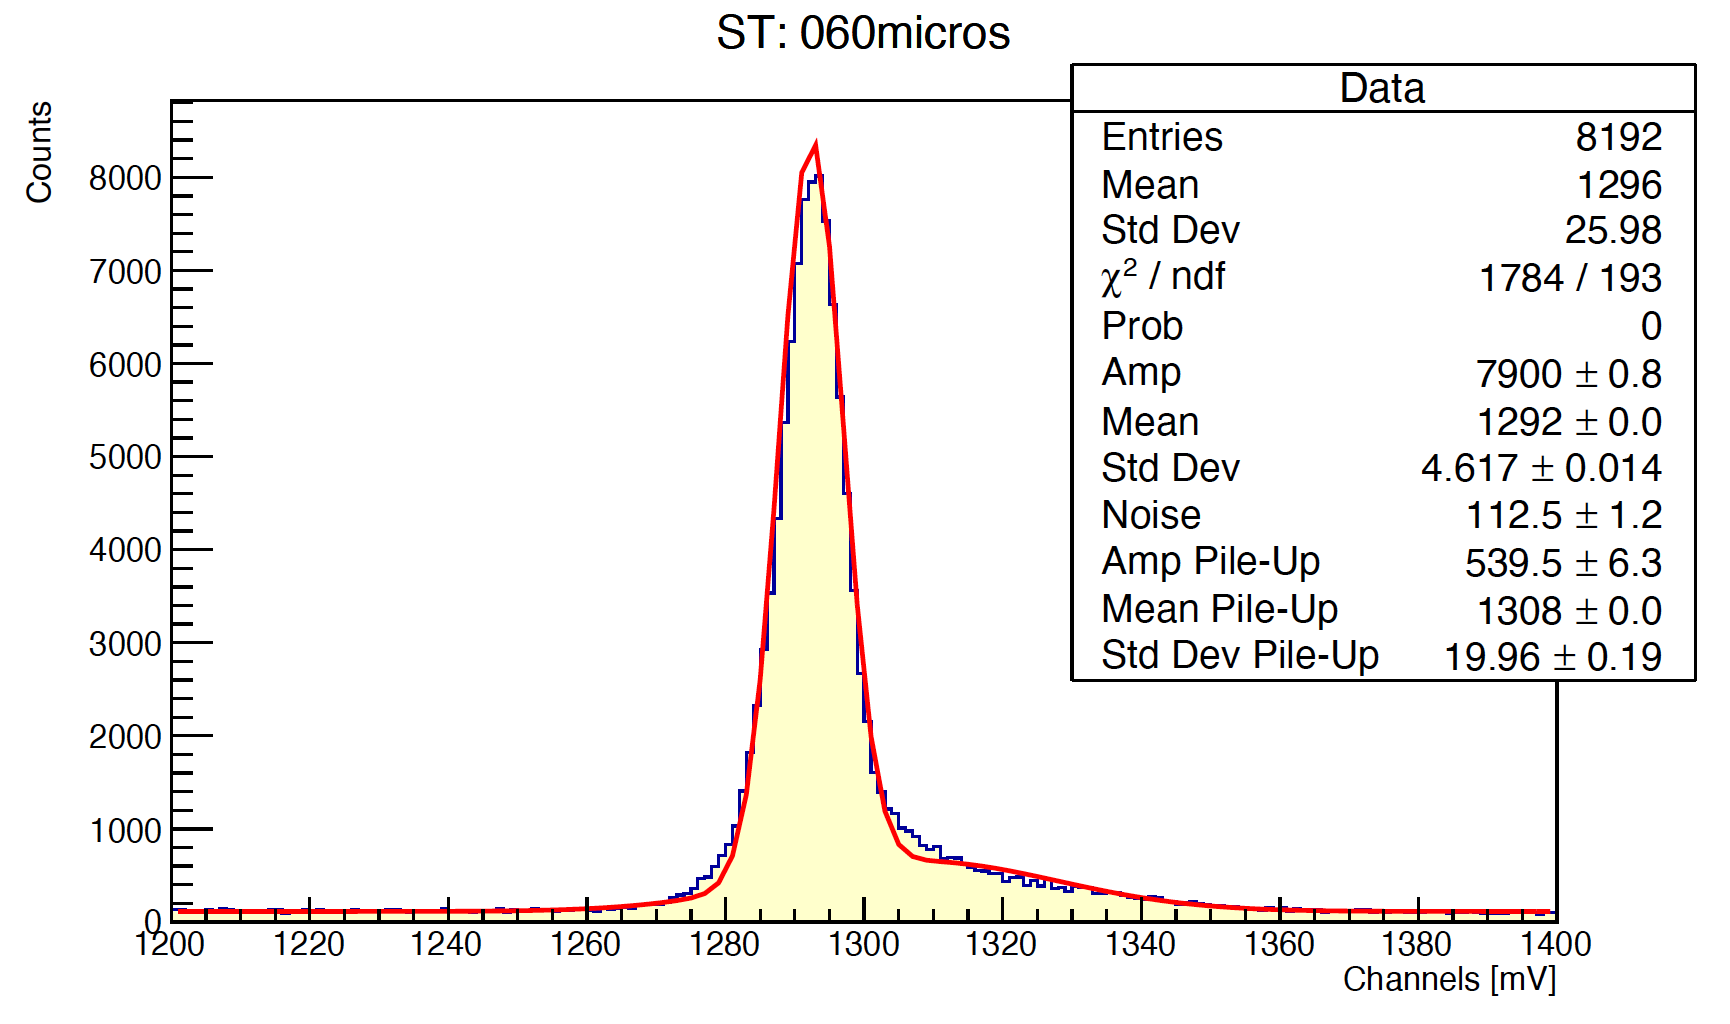
\includegraphics[scale=0.45]{appendice/60}
\end{figure}
\begin{figure}[H]
    \centering
    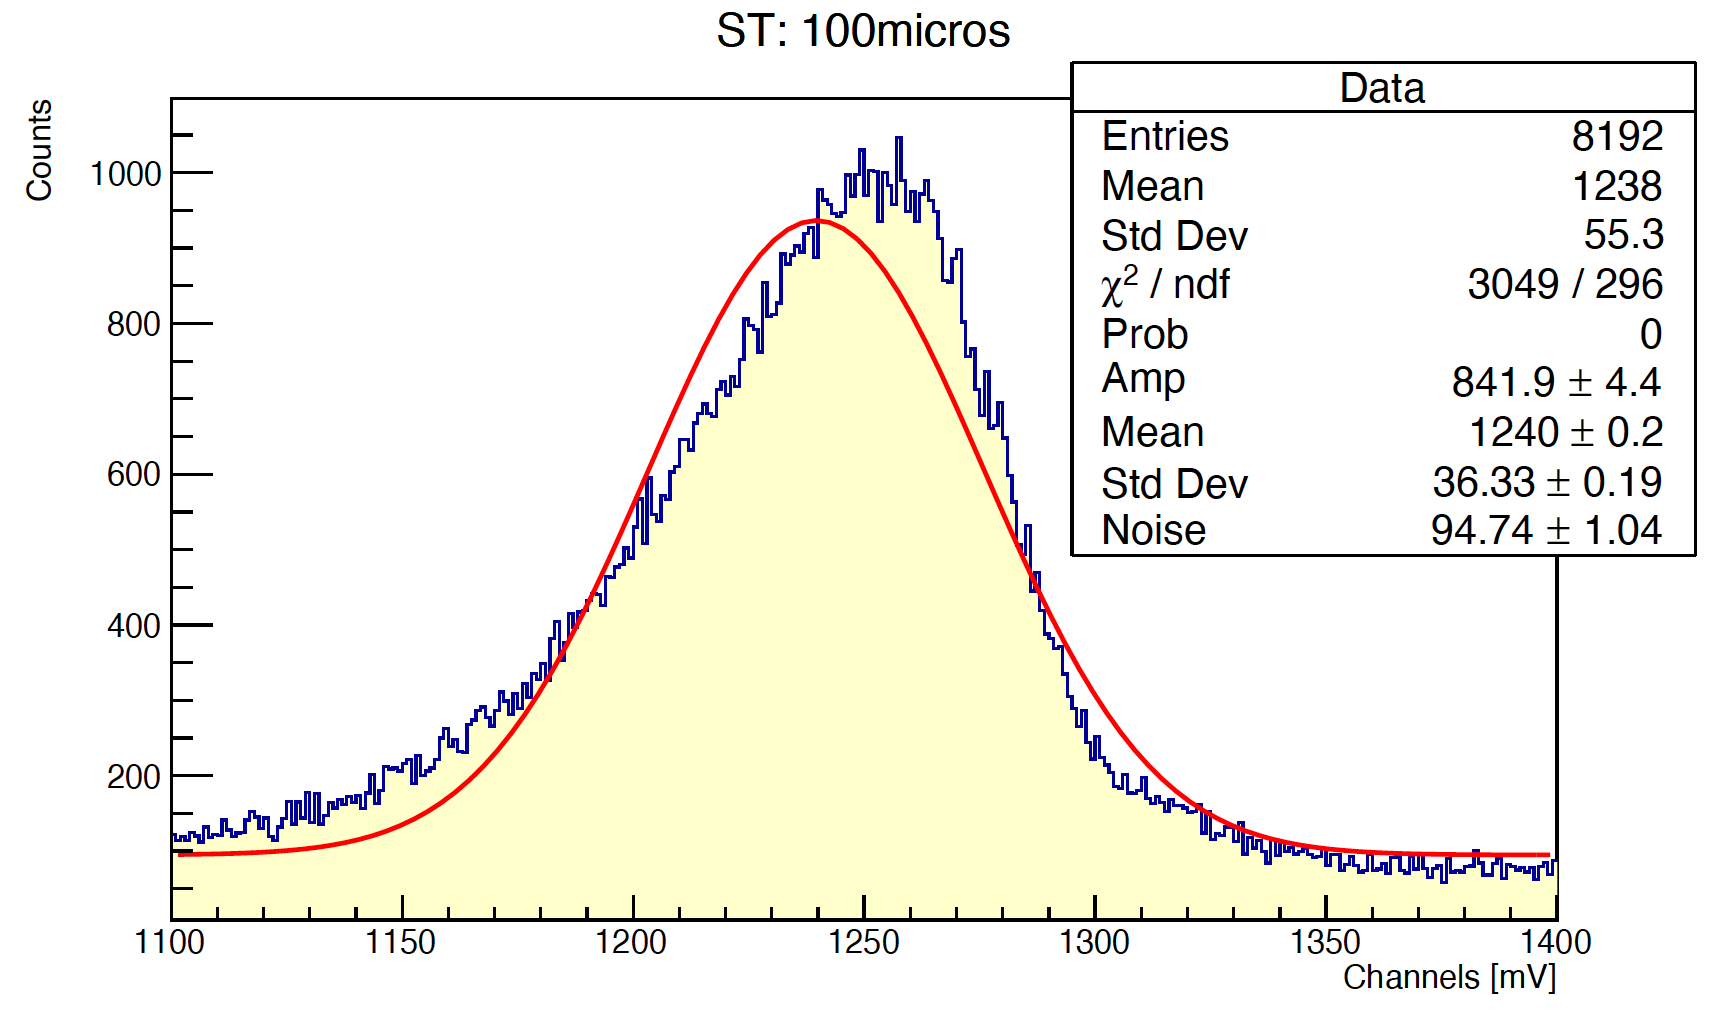
\includegraphics[scale=0.45]{appendice/100}
\end{figure}

%%% PICCHI DEL 22Na %%%
\subsection{Picchi del 22Na}
\begin{figure}[H]
    \centering
    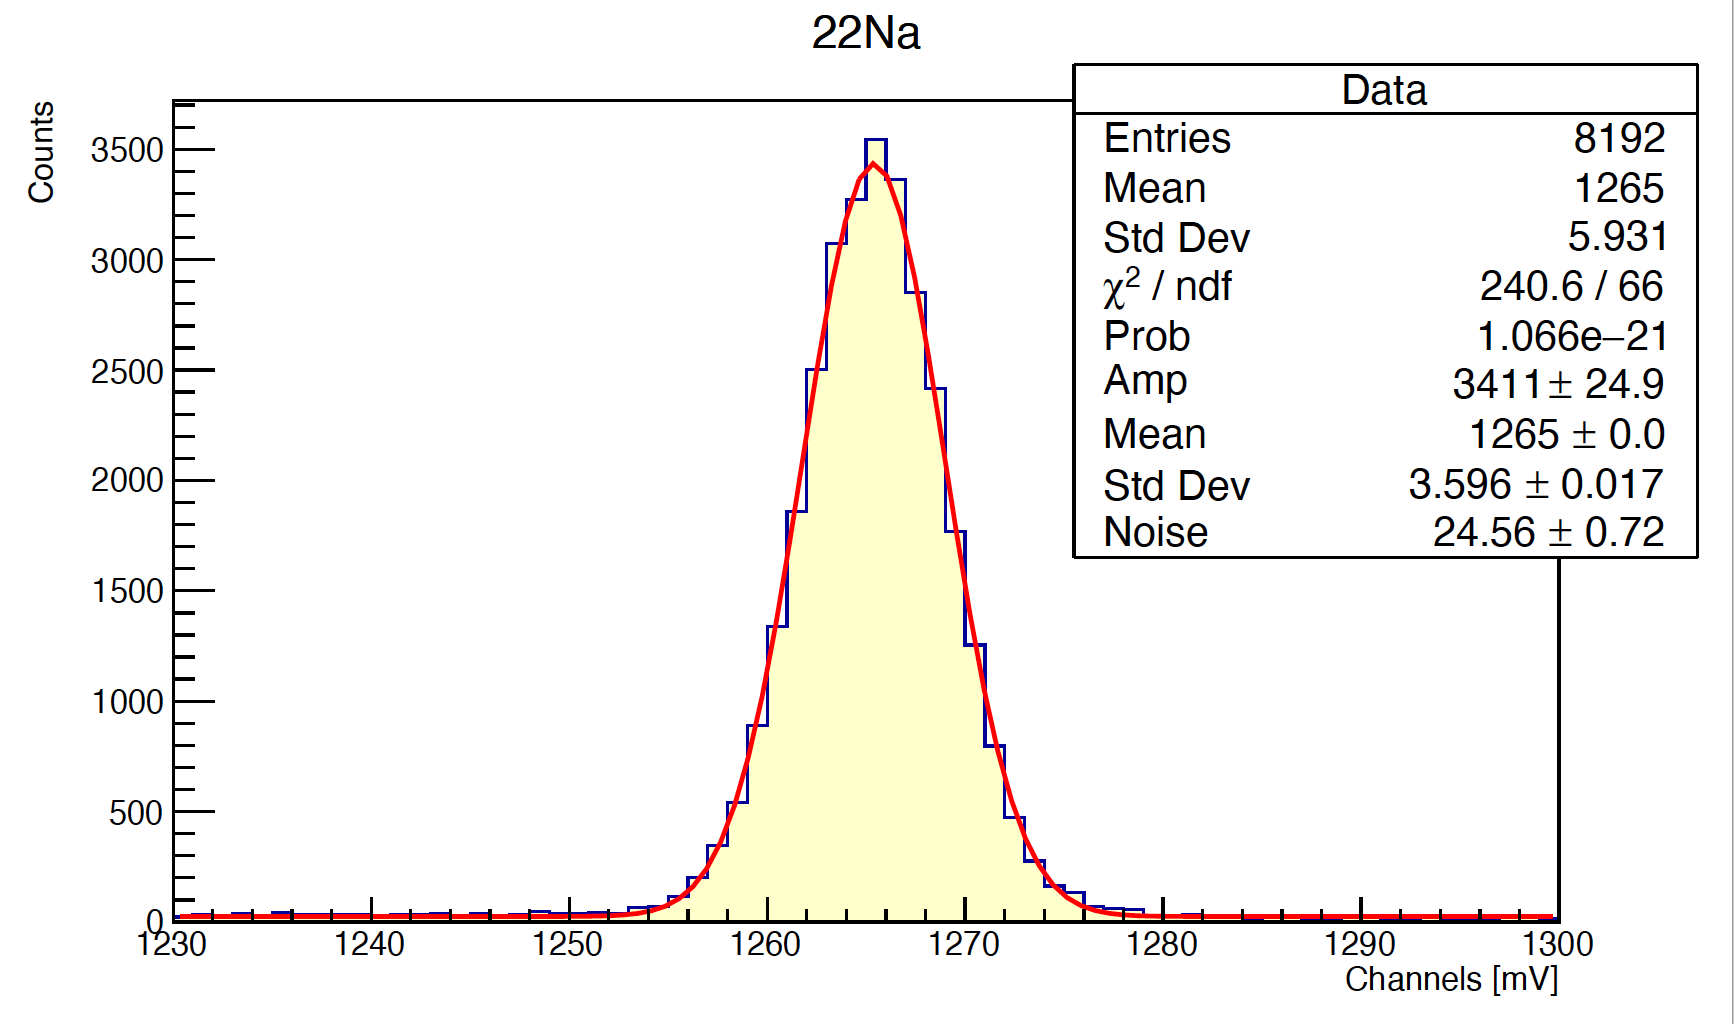
\includegraphics[scale=0.45]{appendice/Na}
\end{figure}
\begin{figure}[H]
    \centering
    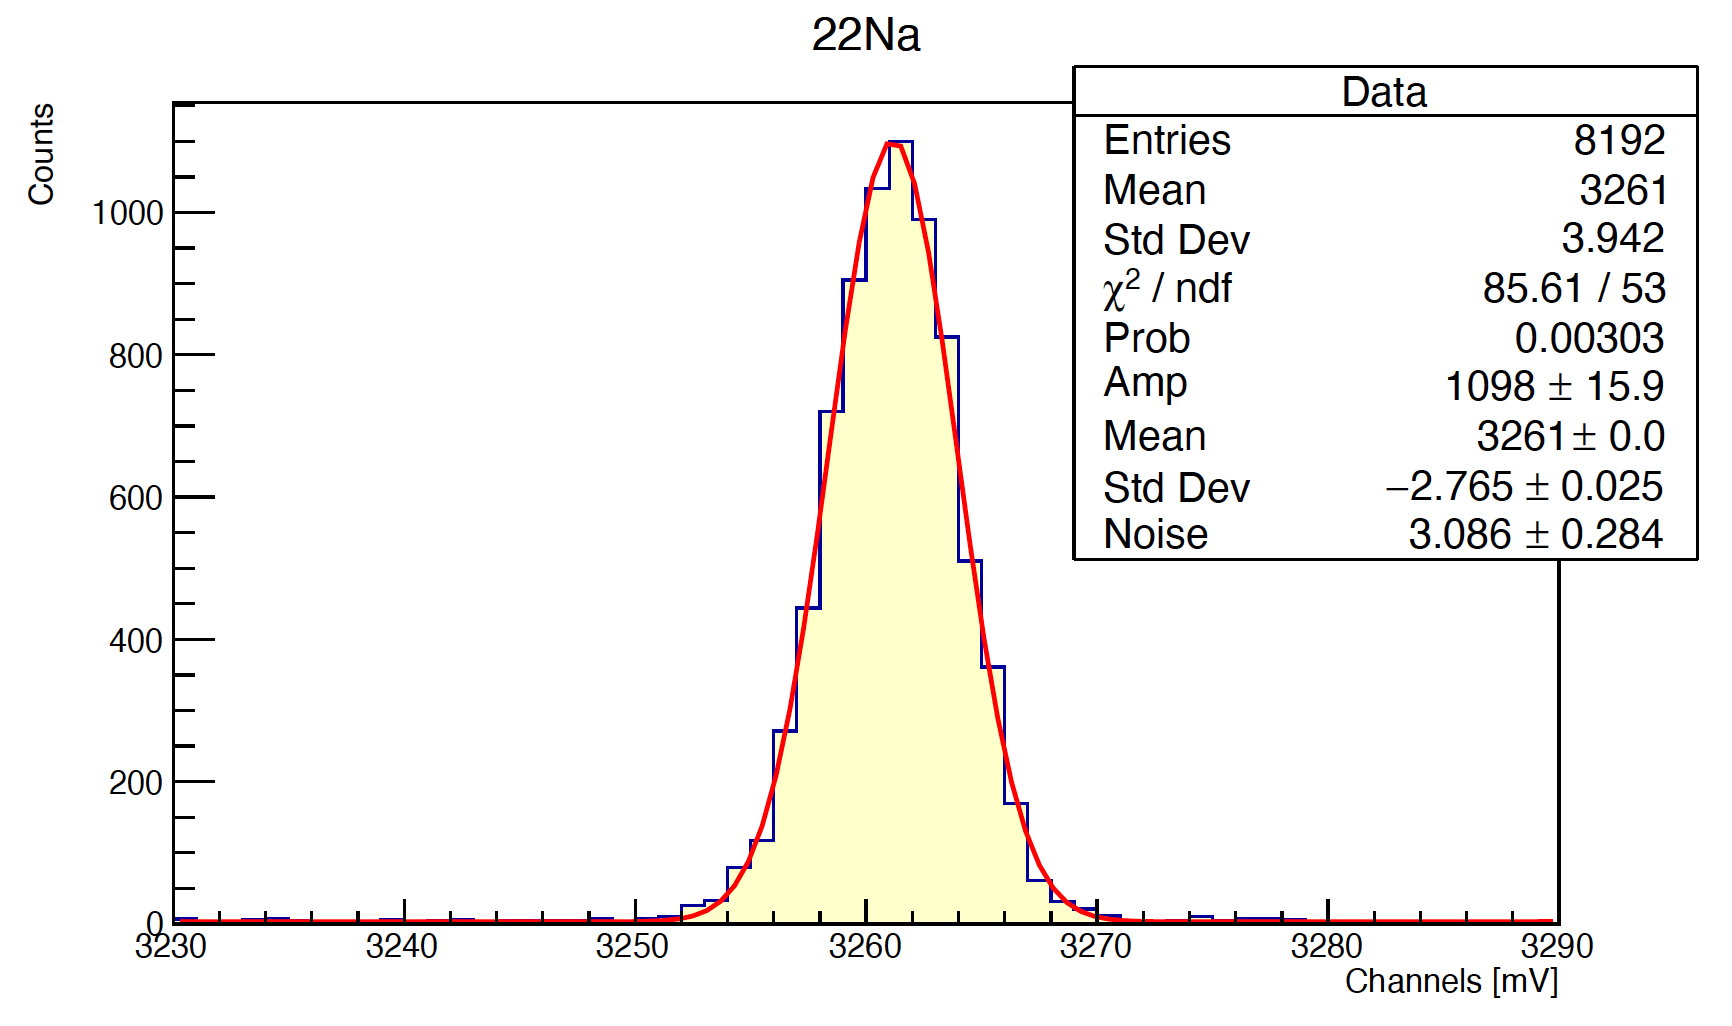
\includegraphics[scale=0.45]{appendice/Na2}
\end{figure}

%%% PICCHI DEL 60Co
\subsection{Picchi del 60Co}
\begin{figure}[H]
    \centering
    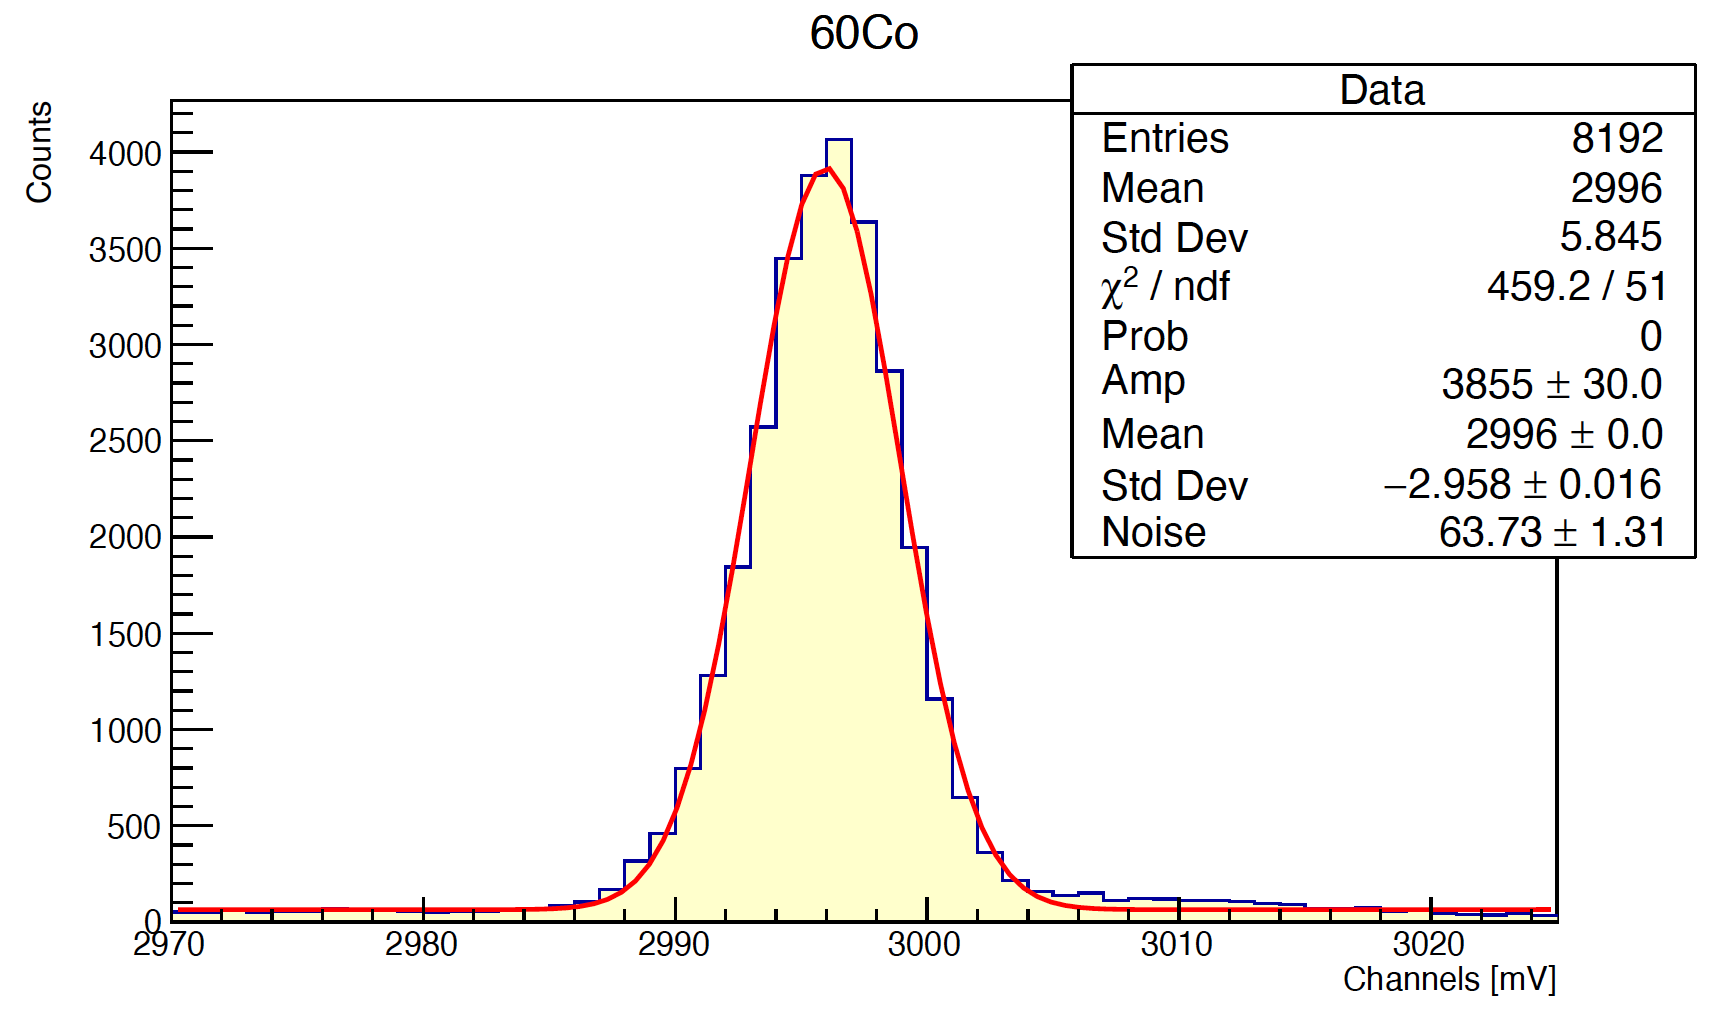
\includegraphics[scale=0.45]{appendice/Co}
\end{figure}
\begin{figure}[H]
    \centering
    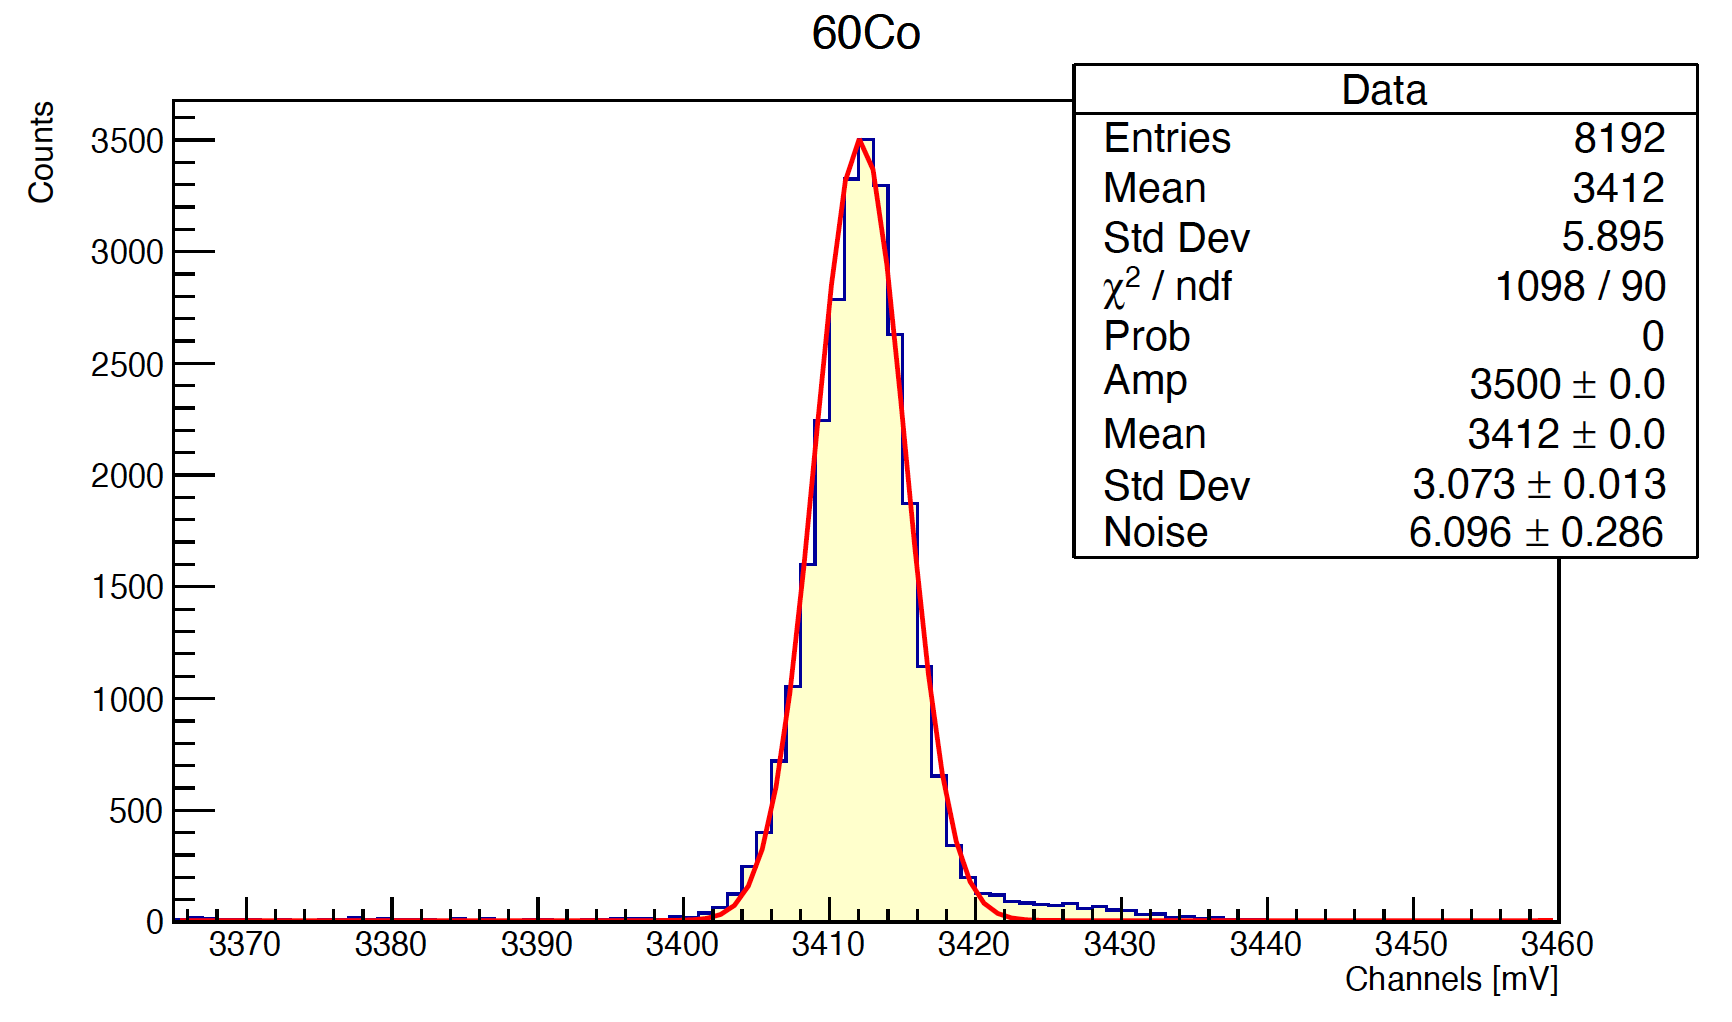
\includegraphics[scale=0.45]{appendice/Co2}
\end{figure}

%%% PICCHI DEL 228Th
\subsection{Picchi del 228Th}
\begin{figure}[H]
    \centering
    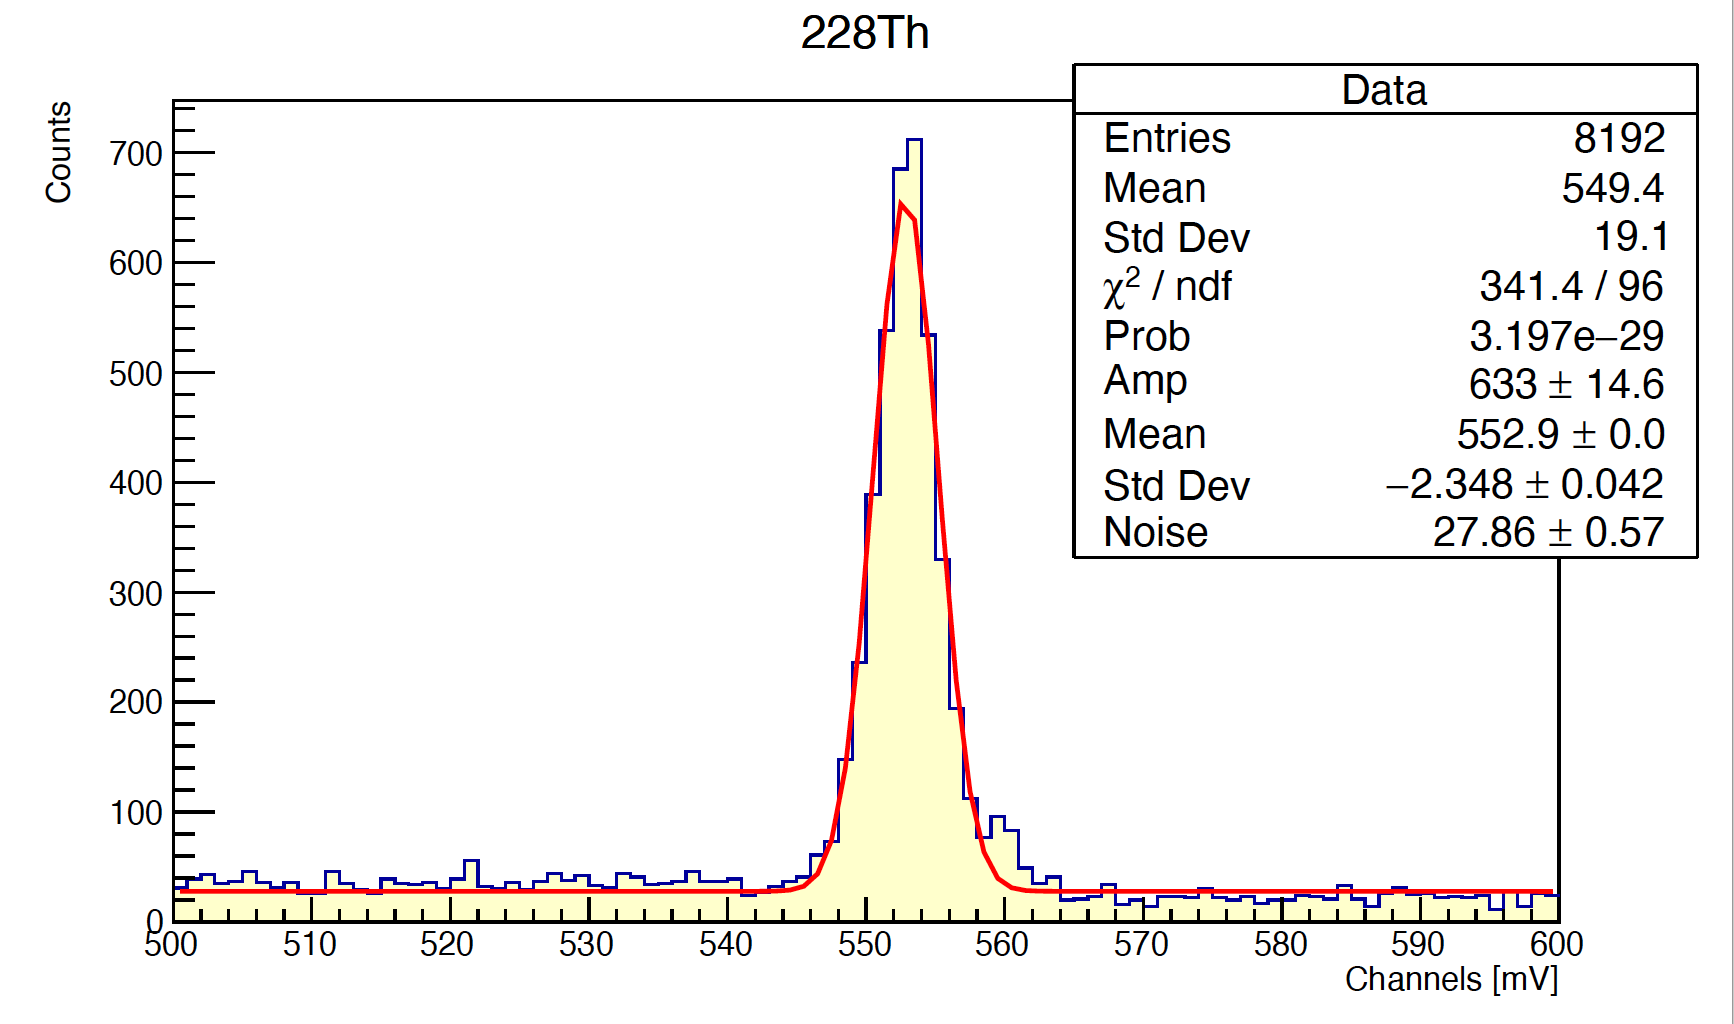
\includegraphics[scale=0.45]{appendice/Th1}
\end{figure}
\begin{figure}[H]
    \centering
    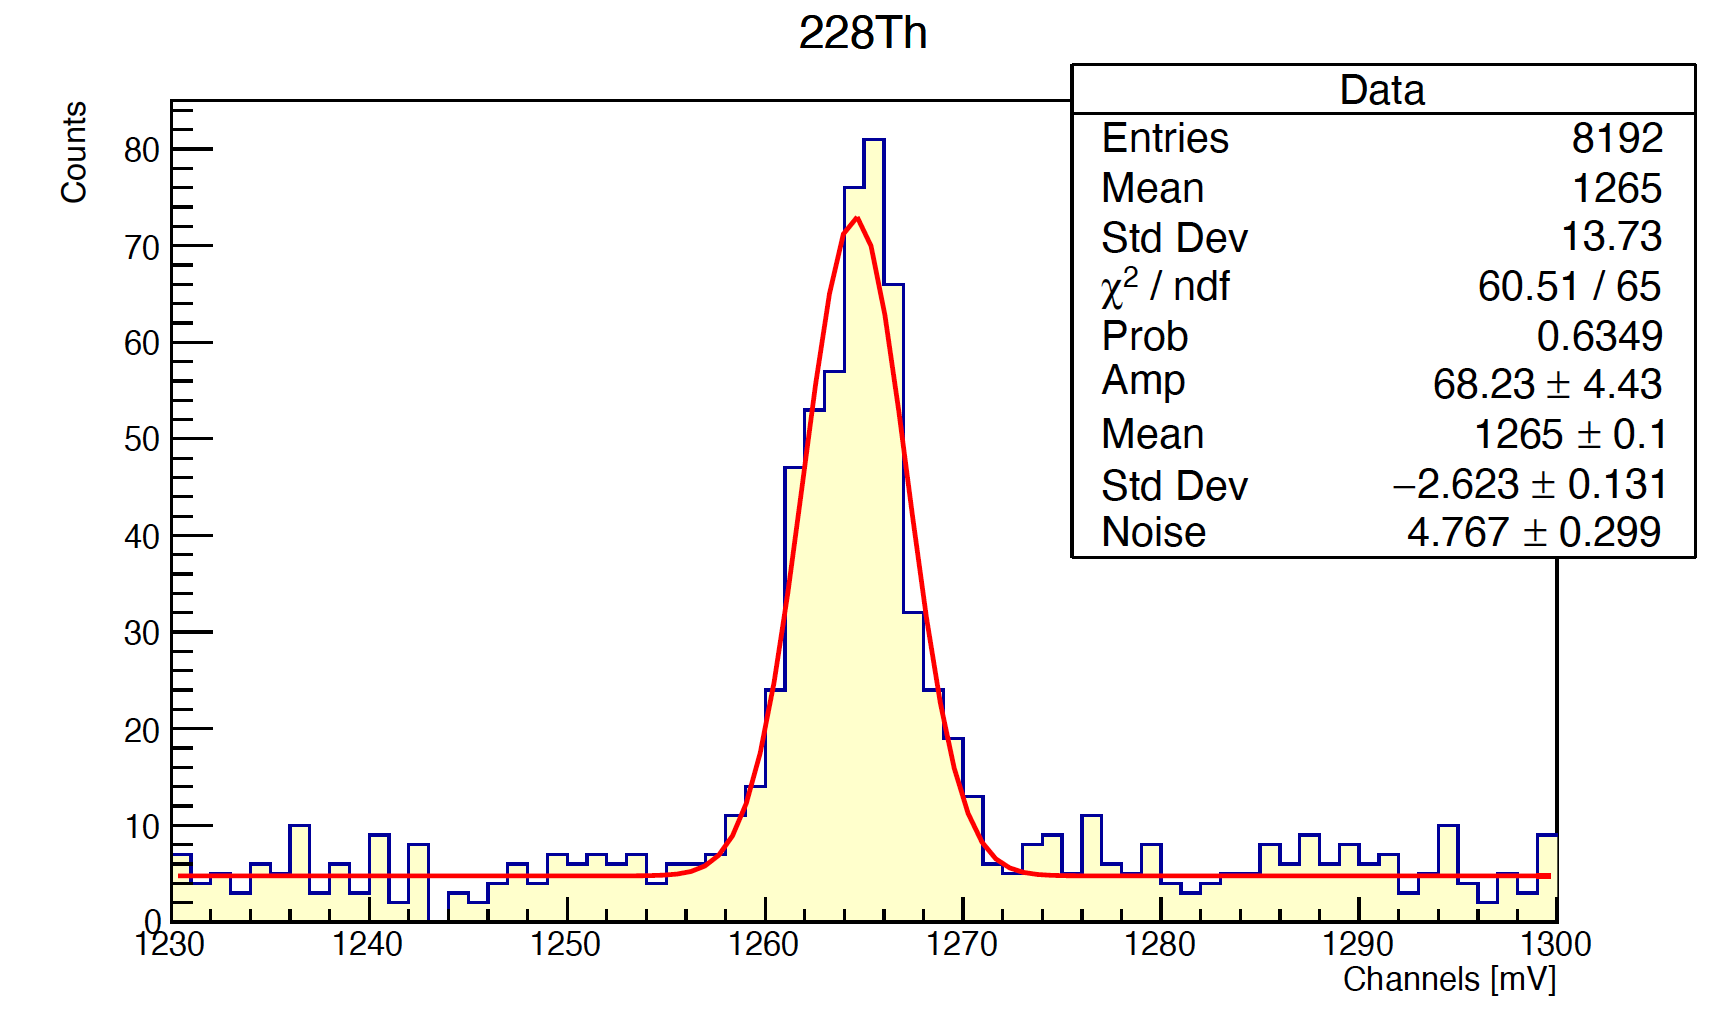
\includegraphics[scale=0.45]{appendice/Th2}
\end{figure}
\begin{figure}[H]
    \centering
    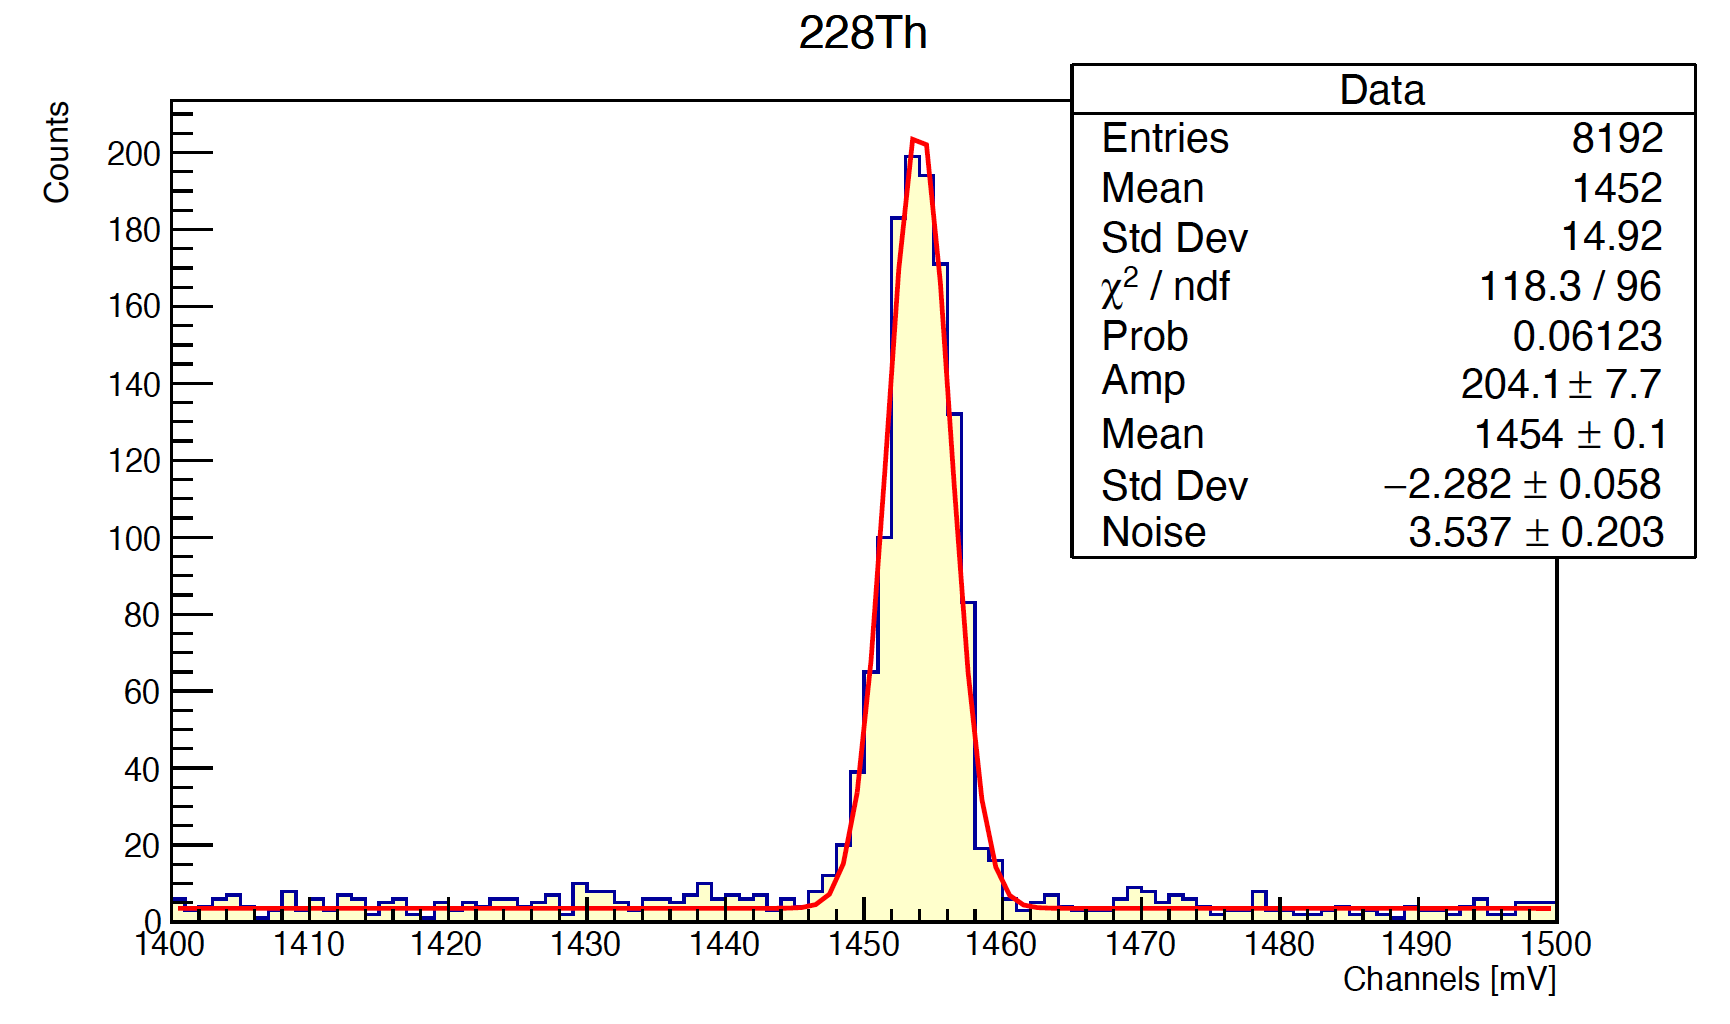
\includegraphics[scale=0.45]{appendice/Th3}
\end{figure}
\begin{figure}[H]
    \centering
    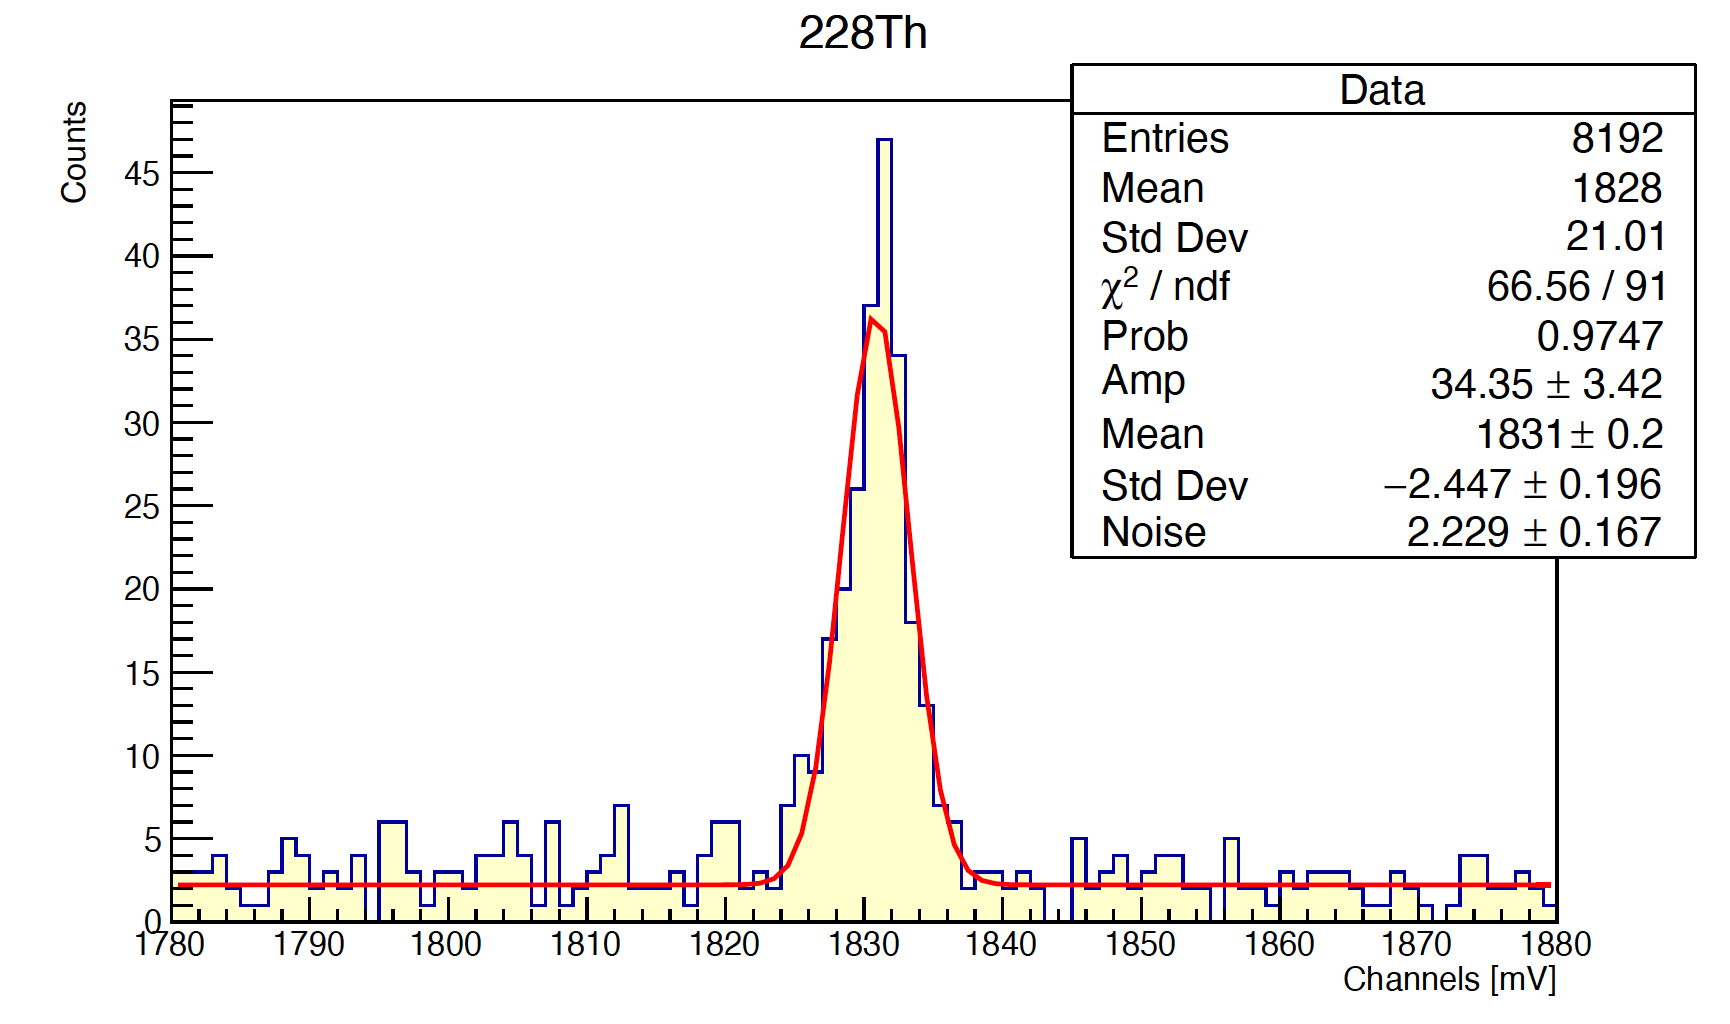
\includegraphics[scale=0.45]{appendice/Th4}
\end{figure}
\begin{figure}[H]
    \centering
    \includegraphics[scale=0.45]{appendice/Th5}
\end{figure}

%%% PICCHI DELLA SORGENTE UW878
\subsection{Picchi della sorgente UW878}
\begin{figure}[H]
    \centering
    \includegraphics[scale=0.45]{appendice/u1}
\end{figure}
\begin{figure}[H]
    \centering
    \includegraphics[scale=0.45]{appendice/u2}
\end{figure}
\begin{figure}[H]
    \centering
    \includegraphics[scale=0.45]{appendice/u3}
\end{figure}
\begin{figure}[H]
    \centering
    \includegraphics[scale=0.45]{appendice/u4}
\end{figure}
\begin{figure}[H]
    \centering
    \includegraphics[scale=0.45]{appendice/u5}
\end{figure}
\begin{figure}[H]
    \centering
    \includegraphics[scale=0.45]{appendice/u6}
\end{figure}

\subsection{Picchi della sorgente ignota}
\begin{figure}[H]
    \centering
    \includegraphics[scale=0.45]{appendice/y1}
\end{figure}
\begin{figure}[H]
    \centering
    \includegraphics[scale=0.45]{appendice/y8}
\end{figure}
\begin{figure}[H]
    \centering
    \includegraphics[scale=0.45]{appendice/y9}
\end{figure}
\begin{figure}[H]
    \centering
    \includegraphics[scale=0.45]{appendice/y2}
\end{figure}
\begin{figure}[H]
    \centering
    \includegraphics[scale=0.45]{appendice/y6}
\end{figure}
\begin{figure}[H]
    \centering
    \includegraphics[scale=0.45]{appendice/y7}
\end{figure}
\begin{figure}[H]
    \centering
    \includegraphics[scale=0.45]{appendice/y3}
\end{figure}
\begin{figure}[H]
    \centering
    \includegraphics[scale=0.45]{appendice/y4}
\end{figure}
\begin{figure}[H]
    \centering
    \includegraphics[scale=0.45]{appendice/y5}
\end{figure}
\begin{figure}[H]
    \centering
    \includegraphics[scale=0.45]{appendice/y10}
\end{figure}


\end{document}